\documentclass[11pt]{article}
\usepackage[margin=1in]{geometry}
\usepackage[utf8]{inputenc}
\usepackage[T1]{fontenc}
\usepackage{lmodern}
\usepackage{microtype}
\usepackage{setspace}
\usepackage{amsmath}
\usepackage{amssymb}
\usepackage{graphicx}
\usepackage{xcolor}
\usepackage[hang,flushmargin]{footmisc}  % no first-line indent on footnotes
\usepackage{hyperref}
\usepackage[round, authoryear]{natbib}
\usepackage{booktabs}
\usepackage{caption}
\usepackage{float}
\usepackage{textcomp}
\usepackage{tikz}
\usepackage{titling}
\onehalfspacing
\usepackage{authblk}
\usetikzlibrary{arrows.meta, positioning, fit, backgrounds, calc, shapes.geometric}
\renewcommand{\_}{\textunderscore\allowbreak}
\setlength{\emergencystretch}{2em}

% APA-style spacing in references
\setlength{\bibsep}{6pt plus 2pt minus 1pt}
\renewcommand{\bibsection}{\section*{References}}

% Hanging indents on references (APA convention)
\bibliographystyle{plainnat}
\hypersetup{colorlinks=true, linkcolor=black, citecolor=black, urlcolor=blue}

% --- TikZ node styles for the process diagrams -----------------------------
\definecolor{gfblue}{HTML}{2A78D6}
\definecolor{gfgreen}{HTML}{2E8B57}
\definecolor{gforange}{HTML}{EB6834}
\definecolor{gfgray}{HTML}{52514E}
\definecolor{gfsand}{HTML}{DED9CC}
\tikzset{
  io/.style   ={rectangle, rounded corners=2pt, draw=gfgray, fill=gfsand!55, line width=0.7pt,
                align=center, inner sep=5pt, font=\footnotesize},
  proc/.style ={rectangle, rounded corners=2pt, draw=gfgray, fill=blue!7, line width=0.7pt,
                align=center, inner sep=5pt, font=\footnotesize},
  headx/.style={rectangle, rounded corners=2pt, draw=gfgray, fill=green!8, line width=0.7pt,
                align=center, inner sep=5pt, font=\footnotesize},
  outbox/.style={rectangle, rounded corners=2pt, draw=gfgray, fill=orange!10, line width=0.9pt,
                align=center, inner sep=5pt, font=\footnotesize\bfseries},
  flow/.style ={-{Latex[length=2.4mm]}, draw=gfgray, line width=0.7pt},
  lbl/.style  ={font=\scriptsize\itshape, text=gfgray},
}

\title{Weather Effects and Heat Acclimation in Endurance Running:\\
A Data Learned Approach to Heat-Adjusted Pace Prediction}
\author{Peter Dunphy}
\author{Thomas Mulc}
\author{Gabe Cupino}
\affil{Kailo, Mountain View, CA, U.S.A.}
\date{\today}

\begin{document}
\setlength{\droptitle}{-2cm} 
\maketitle
\vspace{-1.1cm}

% --- Primer -------------
\begin{center}
\rule{\linewidth}{0.4pt}\\[3pt]
{\large\textbf{Abstract}}\\[1pt]
\rule{\linewidth}{0.4pt}
\end{center}

\begin{singlespace}\small

\noindent\textbf{Motivation.} Anthropogenic warming is making extreme-heat events more frequent, and across the six Abbott World Marathon Majors abnormally hot editions have arrived roughly six times more often per year since 2020 than in the preceding four decades. Finish-time predictors have improved over the same period, drawing on training data collected passively by GPS watches, but they remain weather-blind, and are therefore systematically optimistic on precisely the days when a runner most needs a dependable estimate.

\smallskip
\noindent\textbf{Literature.} Heat slows distance runners nonlinearly, with performance flat through a cool optimum near 10--15\,\textdegree C wet-bulb globe temperature (WBGT) and degrading increasingly above it. The cost is uneven: slower runners lose two to three times more pace per degree than elite fields, and the penalty grows with the duration of the event. Sensitivity also depends on recent exposure, since 5--14 days of heat produces adaptations that decay within weeks. Large observational studies rarely model this individual variation, while the controlled experiments that measure it directly run at 10--30 participants and seldom connect to race performance.

\smallskip
\noindent\textbf{Methods.} We assembled roughly four hundred thousand training runs, each matched to the weather it was run in. A transformer trained on each runner's recent streams predicts pace and, through counterfactual WBGT sweeps, yields a population heat curve derived from inferred per-runner heat sensitivities. Both are added to a weather-blind pace model and evaluated on a runner-disjoint holdout of 24{,}311 activities from 154 runners, using robust error, signed bias, and a direct calibration of each feature. The race-day scale of the curve is then estimated on official results: 1.45 million finishes from 50 editions of five marathons, linked into 268{,}000 repeat finishers.

\smallskip
\noindent\textbf{Results.} The learned heat response steepens above roughly 16\,\textdegree C, reaching a 4.3\% pace penalty at 28\,\textdegree C relative to 10\,\textdegree C on training runs, with individual runners spanning 3.1\% to 5.4\% at the tenth and ninetieth percentiles. Against the official results, within-person finish times track the same curve scaled by a factor of 4.9 (95\% interval 3.4--6.5), so a marathon run at 21\,\textdegree C WBGT costs about 6.5\% of finish time, roughly fourteen minutes for a 3:30 marathoner; no wind or other weather term adds to the curve at race level. Adding these features lowered held-out error only modestly, from 7.56 to 7.33\%. The informative result is calibration: the weather-blind model predicts runs in the hottest band 1.84\% too fast, and the heat features remove that optimism. A shuffled control confirms the personalized gain is runner-specific, but its effect is nearly independent of temperature and its direction reverses once heart rate is conditioned on.

\smallskip
\noindent\textbf{Implications.} Existing work on weather and running performance is retrospective, explaining races already run, while predictors that forecast forward ignore conditions entirely. This study joins the two, predicting pace for a run that has not yet taken place from a runner's prior training and the conditions forecast for it. The population response is well scaled on training runs, its calibrated magnitude matching the correction an independent pace model requires, and its race-day scale is now measured rather than assumed; it is recoverable from data runners already generate. Individualized correction remains unresolved: separating a runner's heat sensitivity from its own physiological consequences will require both a baseline excluding those consequences and race-day performance labels.

\end{singlespace}

\newpage

% Main Document

\section{Introduction}

Anthropogenic climate change has at least doubled the likelihood of record-breaking hot years globally since the late 1960s \citep{king2017}. Over the same period the share of global land area affected by moderate-to-extreme heat waves tripled, and severe heat waves are projected to recur biannually in major population centers by the century's end \citep{russo2014}.

Marathons expose tens of thousands of runners to whatever conditions race day delivers, and the six World Marathon Majors (Boston, London, Berlin, Chicago, New York City, and Tokyo) show a marked increase in the frequency of unusually hot editions. Only three of the 211 races held between 1980 and 2019 exceeded a wet-bulb globe temperature (WBGT) of 65 °F (18 °C), a rate of about 0.08 per year. Three of the 29 races held between 2020 and 2026 already have, a rate of roughly 0.43 per year and a sixfold increase.\footnote{WBGT was estimated using Open-Meteo reanalysis with the Stull (2011) wet-bulb formula and a globe-temperature approximation following \citet{hunter1999}. Fixing the lookup at 10\,am local gives a consistent cross-decade comparison but does not perfectly match on-course exposure, since gun times have shifted over the decades.} The Chicago Marathon is the clearest individual case, with three of its hottest editions falling in the 2020s.

Those conditions confound an already difficult prediction problem. An accurate marathon projection matters to the millions who attempt the distance each year, since it underwrites pacing, goal-setting, and training adjustment. Classic practitioner formulas, including Yasso 800s and VDOT \citep{yasso2008life, gaudette2012yasso, daniels2013running}, remain unpublished in peer-reviewed form decades after their inception. The growth of GPS watches among runners, which track their position, heart rate, and altitude consistently throughout training, offers exciting new pathways for generalizable computational models. 

What every one of these approaches shares, including the predictors now shipped with consumer running platforms \citep{garmin_race_predictor, strava_performance_predictions}, is that it is weather-blind. The literature that does quantify weather effects sits on the other side of the same gap, describing races already run rather than forecasting ones still to come. \citet{vernon2021} documented the cost directly: at the warm 2018 London Marathon (24\,\textdegree C maximum), mass-participation runners finished roughly 47 minutes slower than their pre-race expectations on average, about 14\% off target. A predictor that ignores race-day conditions is therefore systematically optimistic on precisely the days when a runner most needs a dependable estimate.

This paper asks whether that missing weather term can be learned from passively collected training data. We assemble an observational corpus of roughly four hundred thousand training runs, each matched to the weather in which it was run, and train a transformer on each runner's recent training streams to predict pace. Sweeping temperature counterfactually through the trained model yields two quantities: a population heat curve, describing the pace penalty the average runner incurs as conditions warm, and a per-runner sensitivity score, placing an individual within that distribution. We then test whether either improves a weather-blind pace model on runners held out entirely from fitting, and calibrate both against the correction that model actually requires. The population curve proves well scaled and removes the systematic optimism the weather-blind model shows on hot days; the curve also is consistent within existing literature, but demonstrates a novel non-linear heat adjustment learned directly from data; the per-runner score is reproducibly predictive, but its effect is nearly constant across temperature and does not survive conditioning on the physiological signals the baseline already observes. Official race results are then used to measure how much steeper the same curve is on race day than on a training run. Section~\ref{sec:literature} synthesizes the evidence on heat effects and acclimation that motivates this design, Section~\ref{sec:methods} describes the data and the held-out experiment, Section~\ref{sec:results} reports the results, and Section~\ref{sec:discussion} draws out their implications and what remains open.

\section{How Heat Affects Endurance Running Performance}
\label{sec:literature}

Heat degrades endurance running performance through a chain that begins with a physical constraint on heat dissipation, passes through cardiovascular and central strain, and ends in a pacing decision. This section follows that chain, then turns to why the resulting effect is concentrated in endurance events, how it has been measured and modeled, and how it varies across runners.

Running is thermally expensive. Roughly 75\% to 80\% of metabolic energy turnover during exercise appears as heat rather than as mechanical work. That heat must either be dissipated or stored in body tissue \citep{maughan2007}. Storage raises core temperature, and the margin available is narrow, since enzymatic function is near optimal around 39\,\textdegree C while deterioration sets in above roughly 40.5\,\textdegree C \citep{martin2007}. Competitive runners operate close to that ceiling in the heat. Among finishers of the 2019 World Athletics road races, held at WBGT between 23.5 and 30.6\,\textdegree C, 16\% completed their event with a core temperature above 40\,\textdegree C, with a peak recorded value of 40.7\,\textdegree C \citep{aylwin2023}.

Heat balance is an accounting identity, and writing it out locates the constraint. The rate at which heat accumulates in body tissue is whatever metabolic production leaves once the exchange routes have acted,
\begin{equation}
  S \;=\; M \;-\; W \;-\; (R + C + K) \;-\; E,
\end{equation}
with $M$ metabolic heat production, $W$ external work, $R$, $C$ and $K$ radiative, convective and conductive exchange, and $E$ evaporative cooling. In running $W$ is small against $M$ and $K$ is negligible, so storage rises whenever production outruns the sum of the other three. Human tissue has a heat capacity near $3.47\,\mathrm{kJ}$ per \textdegree C, so a sustained imbalance translates quickly into rising core temperature \citep{maughan2010}.

The routes do not contribute equally, and their shares move with conditions. Using the coefficients in \citet{taylor2006}, where convective loss scales as $8.3\,(T_{sk}-T_a)\sqrt{v}$, radiant loss as $5.2\,(T_{sk}-T_{mrt})$ and evaporative loss as $124\,(P_{sk}-P_a)\sqrt{v}$ per square metre, a runner at $5\,\mathrm{m\,s^{-1}}$ with skin at $35\,^{\circ}$C sheds roughly 83\% of its capacity evaporatively at $25\,^{\circ}$C and 50\% humidity, against 14\% by convection and 4\% by radiation. In cool conditions convection matters considerably more, near 24\% at $10\,^{\circ}$C, because the skin-to-air gradient is wide. In genuinely hot conditions it nearly vanishes: at $33\,^{\circ}$C the gradient is only two degrees and convection falls to about 4\%, which is why \citet{taylor2006} sets the dry terms aside entirely in that case.

So evaporation dominates in the conditions this paper is about, and the dry routes matter most exactly where heat is not a problem. Both dry routes also reverse once air temperature exceeds skin temperature, near $36\,^{\circ}$C, beyond which the runner gains heat from the environment rather than losing it \citep{cheuvront2001}. Humidity acts almost entirely through the evaporative term, since it enters the vapour-pressure gradient $P_{sk}-P_a$ directly; its effect on the convective coefficient runs through air density and conductivity, which differ by around one percent between dry and saturated air, and is not material.

Evaporation is capped not by how hard a runner sweats but by how much vapour the air will accept. Modeling world-record performances at $33\,^{\circ}$C and 50\% relative humidity, \citet{taylor2006} calculated a required evaporation of about $4{,}200\,\mathrm{kJ}$ against a maximum achievable evaporation of $1{,}100\,\mathrm{kJ}$, so barely a quarter of the sweat needed for balance could evaporate at all. Sweat beyond that ceiling drips rather than cools, and is fluid lost for no thermal return. Radiation adds a load air temperature does not register: the $73\,\mathrm{W\,m^{-2}}$ difference \citet{cheuvront2021} measured between early and late Boston Marathon start windows is worth roughly one metabolic equivalent of extra heat production for a four-hour finisher.

This is why the performance response to heat is a threshold rather than a gradient. While maximum evaporation exceeds what balance requires, the runner is in compensable conditions, storage stays near zero and warming costs little. Once the requirement exceeds the ceiling the conditions are uncompensable, storage is necessarily positive, and core temperature climbs until the runner slows enough to bring production down. Which regime a given day falls in depends on humidity and radiation as much as on air temperature, which is the physical reason a composite index outperforms the thermometer.

The strain this imposes is cardiovascular before it is thermal, as skin blood flow directed to the surface for cooling competes with muscle for a finite cardiac output. Dehydration compounds the problem: beyond a 2\% loss of body weight, each further 1\% is associated with roughly a 0.4\,\textdegree C rise in rectal temperature during prolonged running. Sweat rates scale with conditions as well, averaging 0.83\,L\,h$^{-1}$ in marathons below 15\,\textdegree C against 1.2\,L\,h$^{-1}$ above it \citep{cheuvront2001}.

For a competitive runner, these strains express themselves in pace. In a simulated half marathon at WBGT 25.8\,\textdegree C, running speed and oxygen uptake fell significantly once core temperature reached about 39\,\textdegree C, which occurred between 6 and 9\,km, after which core temperature plateaued for the remainder of the race \citep{rodrigues2020}. Real race data corroborate this finding. \citet{ely2008} found that the gap between a runner's closing and opening 5\,km pace widened systematically as conditions warmed while \citet{maughan2007} report that post-marathon core temperature correlates with the time for the final 10\,km rather than with the overall finishing time. Core temperature climbs toward a ceiling over the opening miles and is then held near it by the runner conceding speed. Heat, therefore, acts less as a fixed penalty than as a constraint that tightens as the race proceeds that is paid most heavily in the closing stages. 

That accumulation logic extends across events. Comparing seven World Championships from 1999 to 2011, spanning 18.5 to 30\,\textdegree C, \citet{guy2014} found the sign of the effect reverses with distance: sprinters were substantially faster in the heat ($d = 2.4$ and $2.3$ for men at 100 and 200\,m) while the marathon was the most impaired event of all, at $-3.1\%$ for men and $-2.7\%$ for women.

Sports scientists have converged on wet-bulb globe temperature as the most accurate predictor of heat-related performance stress. The standard formula is
\begin{equation}
  \mathrm{WBGT} = 0.7\,T_{\mathrm{nwb}} + 0.2\,T_{\mathrm{bg}} + 0.1\,T_{\mathrm{db}},
\end{equation}
where $T_{\mathrm{nwb}}$ is the natural wet-bulb temperature, measured by a thermometer with a wet cloth wick ventilated by ambient wind and so capturing humidity and air movement together, $T_{\mathrm{bg}}$ is the black-globe temperature, measured inside a matte-black copper sphere and so capturing radiant load, and $T_{\mathrm{db}}$ is ambient air temperature \citep{cheuvront2021}. This weighting follows the physiology of heat's effect on performance described above. It is also recoverable from the heat balance rather than merely calibrated to it. For a runner with wetted skin, the coefficients in \citet{taylor2006} imply a ratio of evaporative to convective transfer of 14.9\,\textdegree C\,kPa$^{-1}$, which is the standard psychrometric constant. Substituting the definition of the wet-bulb temperature into the sum of the dry and evaporative terms removes air temperature and humidity as separate quantities and leaves total heat-loss capacity a function of skin and wet-bulb temperature alone. Along a line of constant wet-bulb temperature the dry and evaporative shares trade off exactly while their sum does not move, so the heavy weight on the wet-bulb term reflects that it carries the information the two variables jointly hold. Appendix~\ref{app:physics} gives the derivation. The most weight corresponds to the humidity-sensitive term, as evaporative capacity is the binding constraint, while dry heat alone is comparatively benign. WBGT has been found to outperform raw air temperature in cross-event comparison \citep{mantzios2022, ely2007, aylwin2023}.  

The exact functional form of the heat penalty remains contested, and Table~\ref{tab:forms} collects those that have been published. Linear models dominate the literature and adequately describe the moderate ranges observed at most major marathons \citep{ely2007, knechtle2019, nikolaidis2019, vernon2021}.\footnote{These moderate ranges are partly an artifact of major marathons being canceled once heat passes a threshold.} A linear form cannot capture the acceleration of the penalty at the hot end, however, and several designs recover it. Quadratic fits appear across single-race and multi-race designs \citep{martin1999, elhelou2012, gasparetto2020}, while the largest synthesis is explicitly piecewise: across 1{,}258 elite races, \citet{mantzios2022} reported a flat band up to 15\,\textdegree C WBGT with performance declining by $0.4 \pm 0.4\%$ per \textdegree C above it. Table~\ref{tab:forms} collects these forms.

\begin{table}[!ht]
\centering
\footnotesize
\setlength{\tabcolsep}{4pt}
\renewcommand{\arraystretch}{1.15}
\caption{Published functional forms relating heat to endurance running performance.}
\label{tab:forms}
\begin{tabular}{@{}p{2.5cm}|p{3.0cm}|p{2.2cm}|p{2.1cm}|p{5.0cm}@{}}
\toprule
\textbf{Study} & \textbf{Field} & \textbf{Temperature variable} & \textbf{Outcome} & \textbf{Form} \\
\midrule
\citet{martin1999} & Elite winners, New York, 21 races & Air temp.\ (\textdegree F) & Winning time (min) & Quadratic: $148.51 - 0.713\,T + 0.00657\,T^{2}$ (men); linear $140.25 + 0.119\,T$ (women) \\
\citet{ely2007} & Elite and amateur, 7 North American marathons & WBGT (\textdegree C) & \% off course record & Linear within performance group; nomogram by finishing position \\
\citet{vihma2010} & Elite and amateur, Stockholm, 29 races & Air temp.\ (\textdegree C) & Finishing-time anomaly & Linear; increment approximately linear in finishing time \\
\citet{elhelou2012} & Elite and amateur, 6 majors, 1.8M finishers & Air temp.\ (\textdegree C) & Running speed; withdrawal rate & Quadratic; withdrawals $0.02\,T^{2} - 0.59\,T + 5.75$ \\
\citet{nikolaidis2019} & Elite and amateur, Boston, 384k finishers & Air temp.\ and WBGT (\textdegree C) & Finishing time & Linear mixed model: $+1$:$53$ per \textdegree C air temp.\ (all finishers) \\
\citet{knechtle2019} & Elite and amateur, Boston, 581k finishers & Air temp.\ and WBGT (\textdegree C) & Finishing time & Linear: $+1$:$47$ per \textdegree C air temp.\ (all finishers) \\
\citet{gasparetto2020} & Elite and amateur, New York, 4 performance clusters & WBGT and UTCI (\textdegree C) & Finishing time (s) & Cluster-specific quadratic: linear $-58.75$ to $-202.9$\,s\,\textdegree C$^{-1}$; quadratic $3.79$ to $13.03$\,s\,\textdegree C$^{-2}$ \\
\citet{vernon2021} & Amateur mass field, London, 676k finishers & Race-day max.\ air temp.; differential vs prior 60-day mean (\textdegree C) & Mean finishing time (min) & Linear: $1.5248\,T_{\max} + 246.52$; $1.4918\,\Delta T + 265.54$ \\
\citet{tan2022} & Elite and amateur, Singapore, 1{,}830 finishers & Dry-bulb and wet-bulb (\textdegree C) & Net time & Log-log elasticity: $+7.6\%$ per 1\% rise in $T_{db}$; $+39.1\%$ per 1\% in $T_{wb}$ \\
\citet{mantzios2022} & Elite championship races, 1{,}258 races, 42 countries & WBGT (\textdegree C) & \% performance decline & Piecewise: flat to 15\,\textdegree C, then $-0.4 \pm 0.4\%$ per \textdegree C \\
\citet{aylwin2023} & Elite, World Championships, Doha & WBGT (\textdegree C) & \% of personal best & Linear: $2.1534\,\mathrm{WBGT} + 52.513$ ($R^{2} = 0.89$) \\
\citet{weiss2024} & Elite and amateur, Berlin, 669k finishers & Air temp.\ (\textdegree C) & Pace (min\,km$^{-1}$) & Linear: $+0.8142$ per \textdegree C; also gradient-boosted trees \\
\citet{llewellyn2025} & Elite and amateur, 6 marathons, USA and Germany & Air temp.\ (\textdegree C) & Median finishing time & J-curve, inflection near 10\,\textdegree C \\
Practitioner rules & Coaching heuristics, reviewed in \citet{montain2007} & Air temp.\ (\textdegree C) & Finishing time & Frederick $\approx 2\%$ per 5\,\textdegree C above 12\,\textdegree C; Daniels $1.6\%$ per 5\,\textdegree C to 32\,\textdegree C; Brown 7--8\% in warm conditions \\
\bottomrule
\end{tabular}
\end{table}

The estimated optimal temperature for endurance running performance is also a source of scholarly contention. Optimal air temperature estimates range from about 3.8 to 9.9\,\textdegree C \citep{elhelou2012} and 5 to 10\,\textdegree C \citep{llewellyn2025} through 10 to 12\,\textdegree C \citep{maughan2010} to 12 to 15\,\textdegree C \citep{martin1999, martin2007}. On WBGT, \citet{mantzios2022} place the marathon optimum at 7.5\,\textdegree C. \citet{gasparetto2020} locate a tipping point near 8\,\textdegree C. This wide span reflects, in part, the vast individual-level differences among runners that together constitute heat tolerance.

The most studied of these individual variations is performance level. Across nearly every large observational study, slower runners lose more pace per degree than faster ones. \citet{ely2007} found that between the coolest and warmest WBGT quartiles, the 25th, 50th, 100th and 300th finishers slowed by 2.6, 3.5, 4.9 and 7.9\% respectively. At the Boston Marathon, \citet{nikolaidis2019} estimated 1 minute 53 seconds of slowing per \textdegree C for all finishers against 38 seconds for the top ten. \citet{knechtle2021b} found that running the New York City marathon in warm temperatures added 7.73 minutes for the average finisher but only 1.87 minutes for top-ten finishers. This finding has been challenged by other studies, however, which find that faster finishes have a strong pace penalty in hot weather \citep{gasparetto2020, knechtle2021a}.

Why slower runners should lose remains unsettled. The simplest explanation is exposure: a runner who is on course longer absorbs more of the day's thermal and solar load and often runs through its hottest hours. Physique supplies a second. Among marathoners with laboratory-measured fitness, percent body fat predicted how far a runner finished from their predicted time in warm conditions ($r = 0.503$) \citep{roach2012}. A third consideration corresponds to heat tolerance. Across marathon studies, faster runners generate more metabolic heat and record a hotter post-race rectal temperature \citep{cheuvront2001}. Elite runners therefore carry the larger thermal load and still lose less time to it. What separates the elite then from the mass field is not a lighter heat burden but a greater capacity to continue running at race pace while carrying it.

Other individual-level variables regarding heat sensitivity have produced mixed results. \citet{elhelou2012} found the performance gap between men and women stable across temperatures and \citet{knechtle2021b} found no significant temperature-by-sex interaction, while \citet{roach2012} and \citet{llewellyn2025} report women finishing further from their predicted times than men in warm conditions. For age, the largest heat effects appear in middle-aged rather than the oldest runners \citep{knechtle2021b, weiss2022a}, a pattern that plausibly reflects racing intensity rather than age itself.

Heat imposes the same thermodynamic accounting on every runner, but not the same constraint: the balance in Equation~1 holds universally while its terms do not, since sweat capacity, body surface area and the mass over which heat is stored all differ between individuals, and two runners in identical conditions can therefore sit on opposite sides of the compensable threshold (Appendix~\ref{app:physics}). The cost heat exacts consequently varies widely. Finishing position, body composition, sex, and age each capture part of that variation---each an observable correlates of a latent heat tolerance. This unobserved quality motivates our approach of inferring heat tolerance from a runner's own history of running in varied conditions rather than using demographic proxies.

\subsection{Heat Acclimation}

The differences described above are semi-sticky attributes of a runner. Performance level and body morphology shift slowly, if at all, across a training block. They describe who a runner is rather than what that runner has recently done. Heat acclimation is different in kind. It is a shorter-term physiological response to a training stimulus, acquired within days and lost within weeks. It is the lever of heat tolerance that a runner can most rapidly and deliberately change.

Repeated exposure to heat produces a coordinated set of adaptations that make the same effort thermally cheaper. Plasma volume expands by roughly 7--18\%, resting core temperature falls, sweating begins earlier and loses less sodium, and skin blood flow responds sooner, so at a fixed workload an acclimatized runner shows a lower heart rate, a lower core temperature, and a lower perceived effort together \citep{periard2015, tyler2016, tyler2024, racinais2017, gibson2020}. The practical consequence is an increased thermoregulatory effect that allows a runner to hold a given pace longer \citep{marino2008, rodrigues2020}. The adaptation can be induced three ways: by exercising in the heat, by passive heating such as sauna or hot-water immersion, or simply by living and training in a hot climate. All three work over a span of about 5--14 days, with hot-climate residence combined with training producing the most complete response \citep{garrett2011, periard2015, tyler2016, tyler2024, heathcote2018, pryor2019, schmit2017, brown2022}.

Research generally agrees on the onset of heat acclimation and its decay. Heart-rate and core-temperature adaptations develop fastest, reaching about 75\% of their eventual gain within 4--7 days; plasma volume expands over 3--6 days; sweat-rate adaptations continue to develop through 10--14 days \citep{periard2015, tyler2016, racinais2020, chalmers2014, cubel2024}. Decay runs on a similar order once exposure stops, at roughly 2.5\% per day for the heart-rate channel, though re-acclimation is considerably faster than initial induction \citep{daanen2018, racinais2020, pryor2019}. A block of 10--14 days therefore captures most of the available adaptation, and a single session every 5--7 days maintains it \citep{daanen2018, garrett2011}. A runner's acclimation state can accordingly be approximated from training-temperature history over the trailing two to four weeks, weighting recent sessions more heavily. Across 29 studies \citet{daanen2018} fit heart-rate decay as $3.6 + 2.3$ per day without heat exposure and core-temperature decay at $2.6$ per day, both in percent of the adaptation gained. Sweat rate behaves differently, since its decay equation carries no term for elapsed days and depends instead on the length and intensity of the original acclimation block, so a longer or hotter block yields a more durable adaptation.

Most large-scale observational studies handle heat adaptation through geographic or fitness proxies such as climate of origin or tropical residence, and almost none fit an individual-level acclimation state \citep{ioannou2018, scheer2021, knechtle2021a, tan2022}. The exception is \citet{vernon2021}, who computed the difference between race-day maximum temperature and each runner's rolling 60-day prior training-environment temperature and reported a correlation of $r = 0.85$ between that differential and mean finish time, with about 2.6\% additional slowdown per 5 °C of positive differential.

Heat acclimation effects are well established in experimental settings. The largest meta-analysis, pooling 1{,}531 participants across controlled trials, reports that acclimation improves subsequent exercise performance and capacity in the heat (Hedges' $g = 0.7$) while lowering resting core temperature ($g = -0.6$) and heart rate ($g = -0.5$) and raising sweat rate ($g = 0.4$) \citep{tyler2024}. Trials in runners recover the same result. \citet{james2017} assigned 17 runners to either short-term heat acclimation or work-matched training in cool conditions, and found the acclimated group improved 5\,km time-trial performance in the heat by 6.2\% against 0.6\% for controls ($p = 0.029$), alongside a 20.8\% gain in total run distance. 

Sustained over years rather than weeks, this dynamic process hardens into something closer to a fixed trait. A runner who lives and trains in a hot climate carries an adaptation that never fully decays, because the exposure never stops. At the Marathon des Sables, a seven-day ultramarathon in the Sahara Desert, athletes from warmer countries ran 10.7\% faster overall than those from colder countries \citep{ioannou2018}. The advantage does not scale indefinitely, however: athletes from the hottest countries of origin, at 25 to 35\,\textdegree C, gained nothing over those from moderately warm countries at 15 to 25\,\textdegree C. Whether that ceiling reflects a limit on useful adaptation or the confounding of origin climate with training resources cannot be settled from the design, but it is consistent with the induction literature above, in which most of the available adaptation arrives well short of the most extreme exposure. Habitual climate, then, is a slow-moving average of exposure, and race-day performance turns on the deviation from it. Measuring that deviation requires knowing the conditions a runner has actually trained in, one session at a time.

\section{Methods}
\label{sec:methods}

\subsection{Design}

The study estimates whether a heat response learned by a deep-learning model improves pace prediction for runners the model has never seen. A weather-blind pace model is fitted first, and heat information is then supplied to it in two stages: a population heat curve that depends only on the conditions of a run, and an individualized, per-runner sensitivity score. Each stage is evaluated on the same runner-disjoint holdout against negative and constrained controls and is separately calibrated against the correction the weather-blind model actually requires. Figure~\ref{fig:pipeline} summarizes the design.

\begin{figure}[!ht]
\centering
\resizebox{0.92\linewidth}{!}{%
\begin{tikzpicture}[every node/.style={align=center}]
  \node[io]    (all)   at (3.5, 0)    {403{,}719 activities from 2{,}420 runners};
  \node[proc]  (split) at (3.5,-1.5)  {Partition by runner identity};
  \node[io]    (fit)   at (0.5,-3.2)  {Fitting runners};
  \node[io]    (hold)  at (6.8,-3.2)  {Holdout runners\\24{,}311 activities, 154 runners};
  \node[headx] (dl)    at (0.5,-5.3)  {Deep-learning heat artifacts:\\population curve,\\per-runner percentile};
  \node[proc]  (prog)  at (0.5,-7.9)  {Pace models\\\textbf{1.} weather-blind\\\textbf{2.} $+$ population curve\\\textbf{3.} $+$ per-runner percentile};
  \node[io]    (ctl)   at (6.8,-7.9)  {Controls:\\shuffled percentile,\\curve-constrained deviation};
  \node[outbox](eval)  at (3.5,-10.4) {Held-out MAPE and bias,\\calibration of $\alpha$ and $\gamma$};
  \draw[flow] (all) -- (split);
  \draw[flow] (split) -| (fit);
  \draw[flow] (split) -| (hold);
  \draw[flow] (fit) -- (dl);
  \draw[flow] (dl) -- (prog);
  \draw[flow] (ctl) -- (prog);
  \draw[flow] (prog.south) |- (eval.west);
  \draw[flow] (hold.east) -- (10.2,-3.2) -- (10.2,-10.4) -- (eval.east);
\end{tikzpicture}}
\caption{The experimental design. Runners are partitioned by a hash of their identifier, so the 154 holdout runners contribute to no fitting stage: neither the deep-learning model, nor the population heat curve and percentile scale derived from it, nor the pace models themselves. Heat information is added to a weather-blind pace model in two steps, first as a population curve that depends only on the conditions of a run and then as a percentile score that depends on the runner. Two controls test whether the second step is genuinely runner-specific: one reassigns each percentile to a different runner, the other forces personalization to act through the temperature curve. All models share the same holdout, hyperparameters and three random seeds.}
\label{fig:pipeline}
\end{figure}

\subsection{Data}

The corpus consists of outdoor running activities recorded on wrist wearable devices by athletes who consented to the research use of their data. Activities were kept only if pace, WBGT and every baseline feature were present. Mean heart rate had to fall between 60 and 210\,bpm and mean pace between 2.5 and 11.5\,min\,km$^{-1}$, which removes sensor dropouts and GPS artifacts without reference to the weather. Runs above 28\,\textdegree C WBGT were excluded, since the corpus thins sharply beyond that point (Appendix~\ref{app:ceiling}). The resulting frame holds 403{,}719 activities from 2{,}420 runners across roughly one hundred countries. This is an enlarged corpus relative to an earlier round of this study: weather enrichment was extended to activities recorded after the original cutoff and to runners who later backfilled their histories, which raised the number of runs above 28\,\textdegree C WBGT from 1{,}846 to 4{,}205 and made the 28\,\textdegree C ceiling supportable.

The target variable, $y_{a,i}$, is the mean pace of activity $i$ for runner $a$, in minutes per kilometer. Runners were split by identity rather than by activity, so no runner contributes to both fitting and evaluation. One runner in ten was held out, leaving 24{,}311 activities from 154 runners for evaluation once the prior-history requirement described below is applied.

\subsection{Weather enrichment}

Weather was sampled from Open-Meteo along each run: once at the start, once at the finish, and every 15 minutes in between, at the runner's location. Each sample gives an outdoor WBGT that accounts for measured solar radiation and wind alongside air temperature and humidity, so that sun and airflow are represented rather than assumed. Each run is then summarized by $\bar{W}_{a,i}$, the time-weighted mean of those samples, rather than by its starting value. Thermal strain accumulates over a run, so a morning start in cool air that finishes in midday heat is described by neither endpoint alone.

\subsection{Deep-learning heat model}

Heat features come from a transformer trained on each runner's recent training streams, a factored-attention network adapted from an existing fitness-prediction architecture. Its input is a window of the 30 most recent activities, each resampled to 128 points and represented by eleven channels: date, latitude, altitude, cadence, cumulative elevation, distance, heart rate, power, activity type, outdoor WBGT, and pace. Each channel is tokenized and embedded separately; the embeddings are summed with a $1/\sqrt{C}$ scale and layer-normalized, and the result passes through attention that mixes information both within an activity and across the runner's recent activities. The model predicts pace directly. It was trained for five million optimizer steps on the fitting runners: an initial one-million-step run, resumed from its final state with the learning-rate decay stretched so that the rate reached its floor at the five-million-step mark rather than at 2.2 million. The checkpoint with the lowest held-out error, at step 4.33 million, is the one used throughout. Two heat artifacts are then read off the trained model by counterfactual WBGT sweeps that hold every other channel fixed.

The \emph{population heat curve} gives the average pace penalty as a function of conditions alone. Each fitting runner's swept response is anchored at $10\,^{\circ}$C and divided by that runner's own value at $28\,^{\circ}$C, isolating the shape of the response from its size. The median of these shapes is taken across the 1{,}786 fitting runners with a positive heat response, then rescaled by the median sensitivity of a 1{,}093-runner reference sample. The model is given no monotonicity constraint, so the shape of the response is whatever the network produces; a monotone projection is applied to the median shape when the published curve is assembled, and Section~\ref{sec:results} reports how much it changes. All reported curves are truncated at 28\,\textdegree C, a limit set by data support rather than by the model; Appendix~\ref{app:ceiling} gives the counts, and Appendix~\ref{app:curve} gives the construction in full.

The \emph{per-runner sensitivity score} is each runner's percentile rank of DL-predicted slowdown at $28\,^{\circ}$C relative to $10\,^{\circ}$C, $\mathrm{slowdown}_{28} = 100\,(\mathrm{DL}_{28^\circ}/\mathrm{DL}_{10^\circ} - 1)$. The primary, prospective version uses a strict prior of exactly 15 preceding windows and excludes the target activity, so it is fully prospective.

\subsection{Baseline model and feature progression}

The baseline is a weather-blind XGBoost pace model with no temperature input: current-run average heart rate, trailing 30-day fitted pace, current-run distance, and elevation (gain and grade). The experiment adds the deep-learning heat information in two steps. The population step adds the DL population curve's value at the run's WBGT as one feature, which the tree model is free to use or ignore. The personalized step additionally adds the runner's sensitivity score. Two controls test what the personalized step is capturing. A shuffled control reassigns each runner's sensitivity score to a random runner, so any genuine personalization gain should vanish. A constrained variant supplies only the percentile-matched deviation of the DL curve, which forces personalization to act through the temperature curve rather than as a free runner-level number. A supplementary branch (Section~\ref{sec:results}) replaces the heart-rate-and-trailing-pace baseline with the fixed, independently-trained marathon-fitness estimate plus distance and elevation, to test whether the findings survive a deliberately different, pre-run baseline.

\subsection{Experimental setup}

All comparisons use the same 24{,}311-activity holdout, identical hyperparameters, and three random seeds (100, 200, 300). Diagnostics computed on the fitting runners use five-fold cross-validation with folds formed by runner.

Two error measures are reported. Let $r_{a,i} = (y_{a,i} - \hat{y}_{a,i})/y_{a,i}$ denote the relative error of a prediction, signed so that a positive value means the run was predicted faster than it was actually run. Accuracy is summarized by a robust mean absolute percentage error,
\begin{equation}
  \mathrm{MAPE} = \frac{100}{n}\sum_{a,i} \min\!\left(|r_{a,i}|,\; q_{99}\right),
\end{equation}
in which $q_{99}$ is the 99th percentile of the absolute relative error, and calibration by the signed bias, the mean of $100\,r_{a,i}$ with the same trimming applied at the 1st and 99th percentiles. Trimming is applied identically to every model. Both measures are needed because they answer different questions: MAPE describes the typical size of an error, whereas bias describes whether a model is systematically optimistic, which is the failure mode that matters on a hot race day. Because activities from the same runner are not independent, all confidence intervals come from a bootstrap resampling runners rather than activities.

Prediction error alone cannot establish whether a heat feature points in the physiologically expected direction, since a flexible tree model can exploit a feature of either sign. We therefore fit a direct affine calibration of the two heat artifacts against the correction the weather-blind prediction requires. The calibration is estimated out-of-fold on the fitting runners, a pool of 227{,}908 activities from 1{,}413 runners, and then frozen before being applied to the holdout, so that no held-out observation informs the coefficients it is later used to judge. The form is
\begin{equation}
  \hat{y} = \hat{p}_0\left(1 + \beta + \alpha\,c_{\mathrm{pop}} + \gamma\,d_{\mathrm{pers}}\right),
\end{equation}
where $\hat{p}_0$ is the weather-blind prediction, $c_{\mathrm{pop}}$ the population curve evaluated at the run's WBGT, and $d_{\mathrm{pers}}$ the personalized deviation. Two coefficients carry the interpretation: $\alpha$ is the scale of the population curve, with $\alpha \approx 1$ indicating that the curve is already of the right magnitude, and $\gamma$ is the direction of the personalized deviation, with $\gamma > 0$ indicating that a runner assigned a larger predicted slowdown does in fact require a slower prediction.

\subsection{Race-day validation data}
\label{sec:raceday_methods}

The corpus is training runs, so the curve it yields is a training-run curve. To measure its scale on race day, official finish lists were assembled for every 2015--2025 edition of five marathons (New York City, Chicago, London, Boston and Big Sur): 1.45 million finishes across 50 editions, from a public results service, used only as training data and never republished. Finishers were linked into persons across editions and courses on normalised name, sex and a birth-year interval (published ages are exact for some races and age groups for others), with hometown as a tie-breaker; same-edition collisions the tie-breaker cannot separate are dropped. The linkage was checked against the service's persistent member identifier where one is present: among persons with two or more identified finishes, the identifier disagrees in 1.4 to 2.8\% of cases by course, an upper bound on the false-link rate. Within-person edition effects were then estimated per course from the 605{,}000 same-course repeat pairs, $\log(t_b/t_a) = e_b - e_a + \delta\,(\text{years apart}) + \text{age term}$, with person-clustered standard errors and the effects centred within course. Each edition's conditions are the mean outdoor WBGT over the mass-start window at the course centroid from the same reanalysis and WBGT routine as the corpus. The race-day scale is the coefficient $\alpha$ in a weighted regression of the edition effects on the learned curve evaluated at that WBGT, with course and calendar-year fixed effects and weights inverse to the squared standard errors; the 2020 London edition, whose mass field ran virtually, is excluded. The same edition table is used to ask whether any weather component adds to the curve, by a LASSO over race-day components with the curve and the fixed effects left unpenalised, and to estimate a physics-form wind-drag term (Section~\ref{sec:future}).

\section{Results}
\label{sec:results}

Two quantities are read off the deep-learning model and supplied to the pace model in turn. The \emph{population heat curve} answers how much the average runner slows in given conditions, and applies the same adjustment to everyone. The \emph{personalized score} answers where a particular runner sits in the spread of heat sensitivity, and adjusts that runner alone. Table~\ref{tab:mainresult} reports the held-out comparison; the sections that follow take each quantity in turn.

\begin{table}[!ht]
  \centering
  \small
  \caption{Held-out model comparison (24{,}311 activities, 154 runners, three XGB seeds). Robust MAPE is clipped at the 99th percentile and signed bias at the 1st and 99th; a positive bias means the run was predicted too fast. Gains are in MAPE points with runner-clustered 95\% bootstrap intervals.}
  \label{tab:mainresult}
  \begin{tabular}{@{}lccl@{}}
    \toprule
    \textbf{Model} & \textbf{Robust MAPE (\%)} & \textbf{Bias (\%)} & \textbf{Gain (95\% CI)} \\
    \midrule
    Weather-blind XGB               & 7.5574 & $-1.53$ & --- \\
    $+$ population DL curve          & 7.4976 & $-1.64$ & $+0.060$ vs blind [0.003, 0.118] \\
    $+$ personalized DL score        & 7.3293 & $-1.17$ & $+0.168$ vs population [0.062, 0.283] \\
    \quad shuffled control          & 7.4841 & $-1.38$ & $+0.014$ vs population [$-0.019$, 0.043] \\
    \quad constrained (curve delta) & 7.3996 & $-1.23$ & $+0.098$ vs population [0.041, 0.154] \\
    \bottomrule
  \end{tabular}
\end{table}

\subsection{The heat response the model learned}

Sweeping temperature through the trained model, holding everything else fixed, traces the pace penalty attributed to heat (Figure~\ref{fig:heat_cost}). The curve is flat through the cool range, turns upward near $16\,^{\circ}$C, and steepens thereafter, reaching 1.0\% at $20\,^{\circ}$C, 2.4\% at $24\,^{\circ}$C and 4.3\% at $28\,^{\circ}$C relative to a $10\,^{\circ}$C reference. These are training-run magnitudes. Expressed as time for a runner whose cool-weather marathon is 3:30 they correspond to roughly two, five and nine minutes, and for a four-hour runner to roughly two and a half, six and ten minutes, if the race were run at training-run sensitivity; Section~\ref{sec:raceday} shows that race-day finish times follow the same curve at about five times that scale. Because the penalty is proportional to time on course, the same conditions cost a slower runner more absolute time, as Figure~\ref{fig:heat_nomogram} sets out across the range of finish times. Held-out error in the hot strata stopped improving between two and two and a half million optimizer steps while overall error continued to fall slowly. The monotone projection applied when the published curve is assembled is immaterial: it alters 6 of 37 grid points, by at most 0.07 percentage points of pace against a 4.2-point range of the median shape. Every individual runner's estimated curve decreases somewhere, yet their median is already non-decreasing to within that tolerance, so the monotone shape is a property the model recovered rather than one assumed.

Individual runners depart from that average substantially. The tenth and ninetieth percentiles of the per-runner response at $28\,^{\circ}$C are 3.1\% and 5.4\%. At training-run scale, for the 3:30 marathoner that is a gap of six and a half minutes versus eleven, and for the four-hour runner seven against thirteen, so a heat-tolerant and a heat-sensitive runner in identical conditions differ by five to six minutes.

\begin{figure}[!ht]
  \centering
  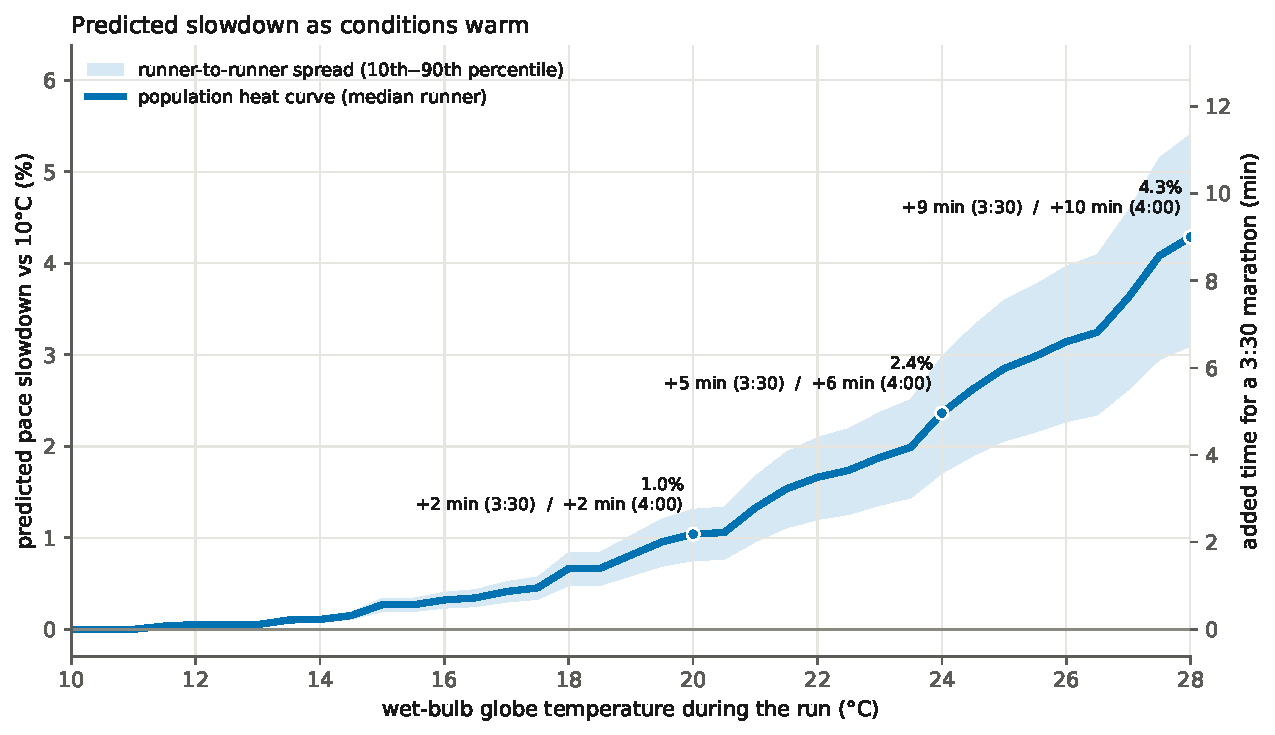
\includegraphics[width=\linewidth]{figures/fig_heat_cost.pdf}
  \caption{The population heat curve estimated by sweeping wet-bulb globe temperature through the trained model. The band spans the 10th to 90th percentile of individual runners' responses. The right-hand axis expresses the same penalty as added finish time for a runner whose cool-weather marathon is 3:30 at training-run sensitivity; race-day finish times scale the same curve by about 4.9 (Section~\ref{sec:raceday}). All values are relative to a $10\,^{\circ}$C reference.}
  \label{fig:heat_cost}
\end{figure}

\begin{figure}[!ht]
  \centering
  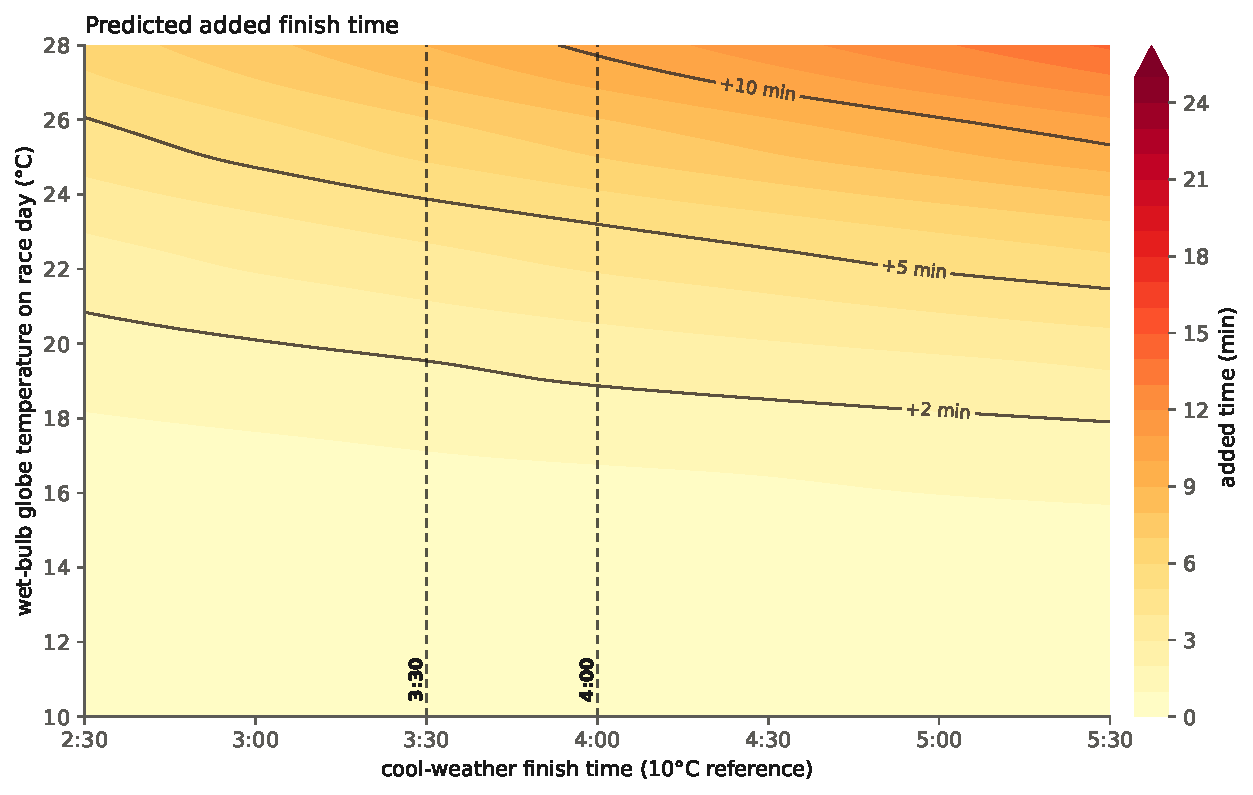
\includegraphics[width=\linewidth]{figures/fig_heat_nomogram.pdf}
  \caption{Predicted added finish time as a function of a runner's cool-weather finish time and the wet-bulb globe temperature on race day. Contours mark round values in minutes. Because the penalty is proportional, contours bend upward to the left: a faster runner must face hotter conditions than a slower one to lose the same number of minutes. The surface is the population curve of Figure~\ref{fig:heat_cost} at training-run scale and carries the same caveats; dashed lines mark the two reference runners used in the text.}
  \label{fig:heat_nomogram}
\end{figure}

Because the curve is estimated without reference to any published result, it can be placed against the existing literature directly (Figure~\ref{fig:heateffects}). The published forms fall into two bands: steep slopes for amateur and mass fields, reaching 10 to 16\% by $30\,^{\circ}$C \citep{ely2007, nikolaidis2019, knechtle2019, vernon2021}, and shallow slopes for elite fields, near 3 to 5\% \citep{mantzios2022, martin1999, guy2014}. The curve estimated here sits at the lower edge of that range. While our model is trained on amateur and mass fields, it also uses training runs, not solely labeled races, and Section~\ref{sec:raceday} shows that this accounts for the lower penalty: on official race results the same curve applies at about five times the training-run scale.

\begin{figure}[!ht]
  \centering
  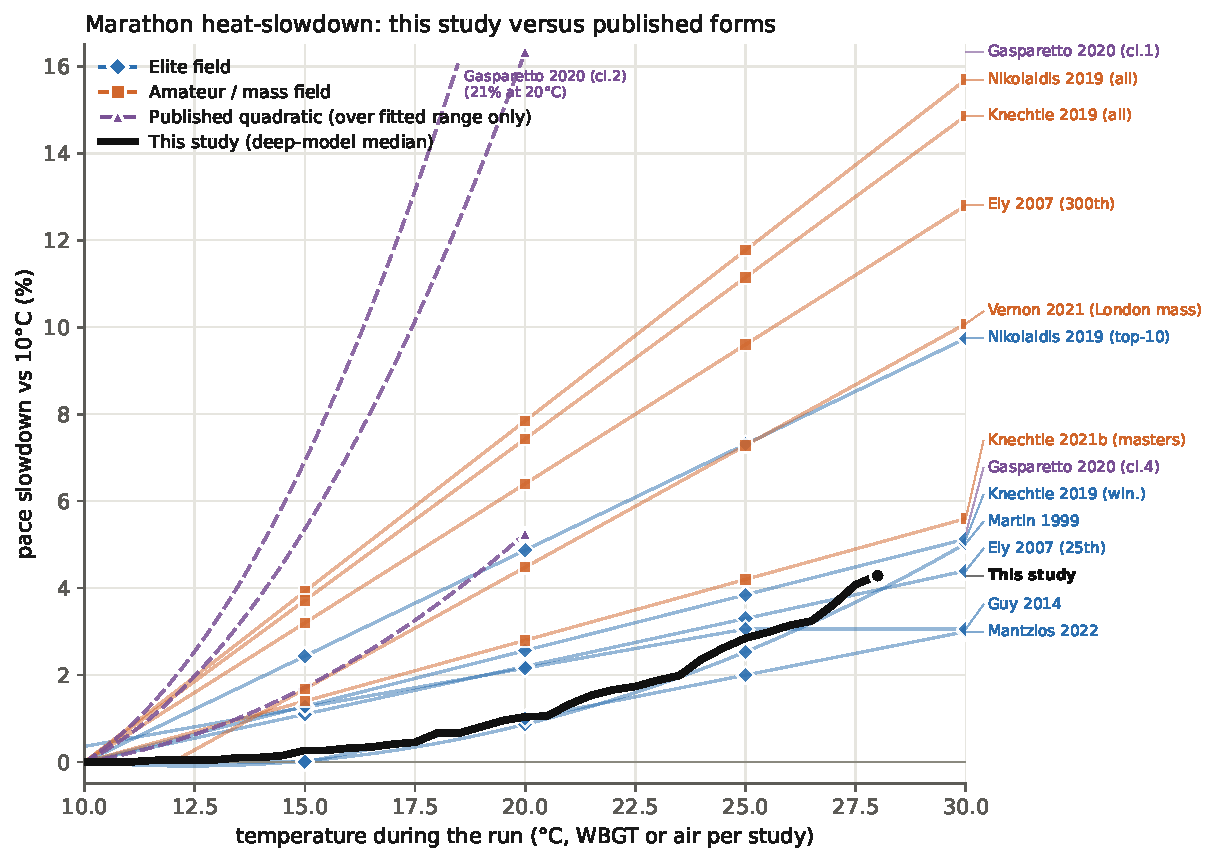
\includegraphics[width=\linewidth]{figures/fig_heat_effects_lit.pdf}
  \caption{The population heat curve estimated here (bold) against published marathon heat-slowdown forms, all expressed as percent pace slowdown relative to a $10\,^{\circ}$C anchor. Marker shape encodes the study population: diamonds for elite fields, squares for amateur or mass fields. Slopes reported in seconds per degree are converted to percent using a representative finish time (elite 130 min, amateur 240 min), and forms native to air temperature rather than WBGT are drawn on the same axis, so placement above about $18\,^{\circ}$C is approximate.}
  \label{fig:heateffects}
\end{figure}

The shape the model settles on is the one the physiology predicts, and it is a shape neither of the two dominant published forms can produce. Below roughly $16\,^{\circ}$C the curve is nearly flat: evaporative capacity exceeds what the runner needs to shed, heat balance holds, and warming costs almost nothing. Above it the curve steepens as the environment's capacity to remove heat falls below the rate of production, so storage accumulates and pace must be conceded. A threshold followed by acceleration is exactly the signature of a constraint that is slack and then binds.

The curvature has a specific physical source, and it is worth stating because it predicts a shape independently of anything the model was shown. The quantity a runner is graded against is the ratio of the evaporation required for heat balance to the maximum the environment will accept, which \citet{taylor2006} term thermal compensability. Its numerator rises close to linearly as conditions warm, because dry exchange is proportional to the skin-to-air gradient and simply reverses sign near $36\,^{\circ}$C. Its denominator falls, and falls at an accelerating rate, because saturation vapor pressure is convex in temperature: it gains between 6 and 7\% of its own value per degree, so the evaporative ceiling sheds about 22\,W\,m$^{-2}$ per degree at a wet-bulb temperature of $12\,^{\circ}$C but about 46 at $26\,^{\circ}$C. A near-linear numerator over a concave denominator is convex, so the physiologically binding quantity must accelerate even though neither of its parts does. For a 70\,kg runner at three-and-a-half-hour marathon effort the required fraction of maximal evaporation rises from 0.12 at a wet-bulb temperature of $15\,^{\circ}$C to 0.82 at $28\,^{\circ}$C, and its increment per degree more than triples across that span. \citet{taylor2006} further note that strain rises gradually as the ratio approaches unity rather than only at the point where it is reached, which matters here: a runner who held pace until the hard limit bound would show almost no penalty and then a collapse, which is not the behavior any measured curve displays.

That argument constrains the shape of the response and not its size, so it can be checked against the learned curve without either one being used to fit the other. Between the 20 to $24\,^{\circ}$C and 24 to $28\,^{\circ}$C bands the learned curve steepens from 0.33 to 0.48\% per degree, a factor of 1.45. The compensability ratio steepens by a factor of 1.80 over the same interval at the reference conditions, and between 1.5 and 2.7 across the humidities and solar loads considered in Appendix~\ref{app:physics}. The two agree in sign and are close in size, with the measured curvature falling just below the range the physics implies. A gap in that direction is consistent with the selection mechanisms of Section~\ref{sec:selection}, all of which act to understate the penalty on the hottest days, and it leaves room for the additional convexity that \citet{taylor2006} attribute to sweat that drips rather than evaporates once the requirement approaches the ceiling. The physics predicts that the curve should bend and roughly how sharply, not that the penalty should reach 4.3\% at $28\,^{\circ}$C. Appendix~\ref{app:physics} gives the calculation.

A linear form cannot represent that threshold at all. It must either overstate the penalty in mild conditions or understate it in hot ones, and the published linear fits do the former, which is visible in Figure~\ref{fig:heateffects} as slopes that rise steadily from $10\,^{\circ}$C where the measured response is flat. A quadratic can bend, but it bends without limit. Fitted over the 8 to $20\,^{\circ}$C range their data spans, the cluster-specific quadratics of \citet{gasparetto2020} already reach 16 and 21\% at $20\,^{\circ}$C for their two fastest clusters, and extrapolating them to $28\,^{\circ}$C would imply slowdowns near 50\%. No runner in the corpus behaves that way. The divergence is a property of the functional form rather than of the data it was fitted to, which is why those curves are drawn here only over the range in which they were estimated.

The learned curve avoids both failures because nothing constrains it to a polynomial. It is flat where the constraint is slack and steepens where the constraint binds, without a polynomial's unbounded growth: above the reported range the raw sweep slows again (Appendix~\ref{app:ceiling}), though that region is too sparsely observed to interpret.

The response is also not a single slope, because it depends on how hard the runner is working.
Estimating the heat slope separately within quintiles of mean heart rate, within runner and with
distance, elevation and fitness controlled, gives $+0.18\%$ per \textdegree C in the easiest fifth
rising monotonically to $+0.44\%$ in the hardest, a factor of 2.4 (Figure~\ref{fig:hrinteraction}).
The gradient is not captured by a linear heart-rate-by-heat interaction
($+0.005\%$ per \textdegree C per standard deviation of heart rate, $t=0.4$), which is indistinguishable
from zero even though every quintile step is in the same direction. The gradient is estimated on the full
corpus; on the 154-runner holdout alone it is not detectable, with overlapping intervals across effort levels. This matters for interpretation
of the population curve, which averages over efforts that are mostly easy, and it is consistent with the
physical account: the compensable threshold is crossed sooner when metabolic heat production is higher,
so the same conditions bind at high effort and not at low.

\begin{figure}[!ht]
\centering
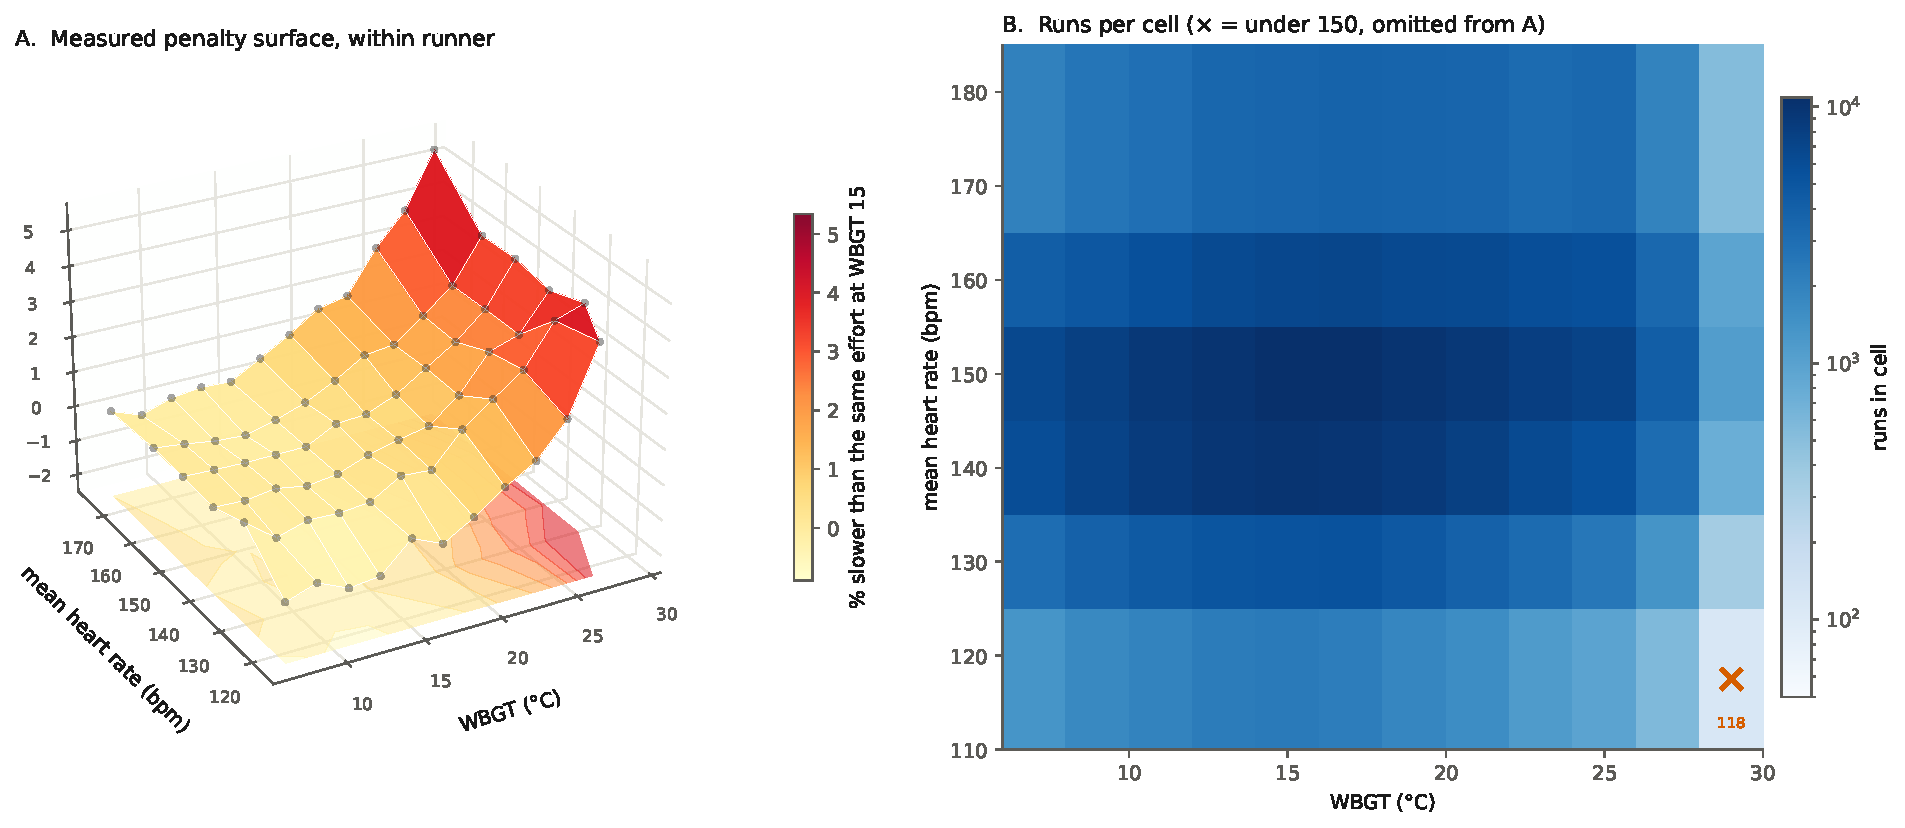
\includegraphics[width=\linewidth]{figures/fig_hr_wbgt_interaction.pdf}
\caption{The pace penalty as a joint function of conditions and effort. \textbf{A:} the surface is
measured rather than fitted. Log pace is residualized within runner on distance, elevation and fitness
(heart rate is deliberately not controlled for, being an axis here), binned on a WBGT-by-heart-rate
grid, and each heart-rate row is expressed relative to its own value at WBGT 15, so the height is the
penalty at a given effort rather than the pace level of that effort. Contours are projected on the floor
for legibility. No functional form is imposed, because the linear heart-rate-by-heat interaction is not
distinguishable from zero and a fitted surface would therefore draw a shape the data does not support.
The plain across cool and easy conditions is flat; the ridge rises only where heat and effort coincide,
reaching roughly $+5\%$ in the hottest and hardest cell; that row (28--30\,\textdegree C) lies above the 28\,\textdegree C ceiling used elsewhere and is shown for completeness. \textbf{B:} runs per cell. Cells below 150 runs
are marked and omitted from A; the hottest-and-hardest cell rests on 534 runs, so the peak of the ridge
is the least certain part of the surface.}
\label{fig:hrinteraction}
\end{figure}

\subsection{Whether weather information improves prediction}

Both heat features lower held-out error (Figure~\ref{fig:mape_ladder}). Robust MAPE falls from 7.56\% for the weather-blind model to 7.50\% with the population curve, and to 7.33\% once the personalized score is added, a total of 0.23 points. On a 3:30 marathon the whole progression is worth about 29 seconds, and on a four-hour marathon about 33. This small magnitude is expected: the effect of heat is a small piece of daily training pace variation, where training intent, terrain and fatigue all have larger effects. Average error over a mostly temperate corpus is therefore a weak instrument for detecting it.

A negative control establishes that the personalized gain is runner-specific rather than an artifact of supplying the model one more numeric feature. The control reuses the personalized percentile with its distribution intact, reassigning each value to a different runner within the fold, so only the pairing between a runner and their own heat response is broken. If the gain came from the extra column alone, the shuffled version should reproduce it; instead it lands at 7.48\%, within noise of the population model. In runner-clustered bootstrap terms, the personalized gain beyond the population curve is 0.168 points, with a 95\% interval of [0.062, 0.283] excluding zero, while the shuffled interval [$-0.019$, 0.043] straddles it. The population curve's own gain of 0.060 points has an interval of [0.003, 0.118], which now excludes zero on the enlarged corpus. The current-inclusive, prior and strict-prior versions of the personalized score perform almost identically, so the gain does not depend on including the target activity.

\begin{figure}[!ht]
  \centering
  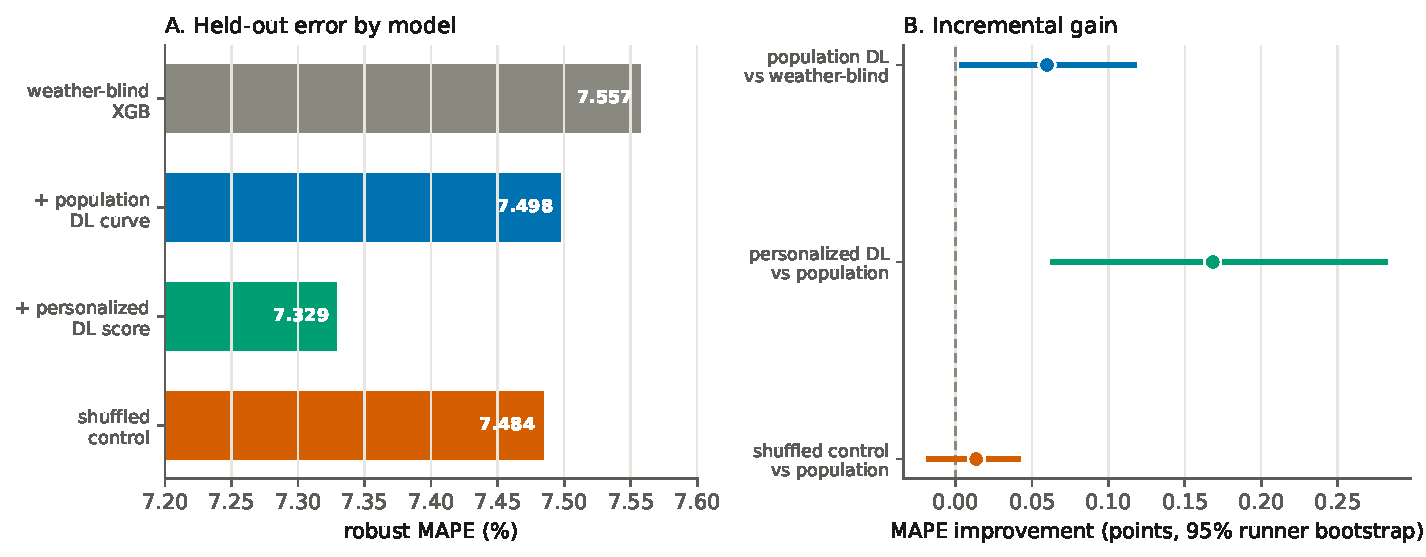
\includegraphics[width=\linewidth]{figures/fig_mape_ladder.pdf}
  \caption{Held-out model comparison (24{,}311 activities, 154 runners, three XGB seeds). Panel A: robust MAPE for each model, where lower is better. Panel B: incremental MAPE improvement with runner-clustered 95\% bootstrap intervals. The personalized gain over the population curve excludes zero, while the shuffled control does not, so the personalization depends on matching the score to the correct runner.}
  \label{fig:mape_ladder}
\end{figure}

\subsection{Limitations of the weather-blind model}

Stratifying held-out error by temperature exposes a systematic failure that average error conceals (Figure~\ref{fig:bias_fix}). The weather-blind model predicts runs too slow in cold and mild conditions, with a bias near $-2\%$, then crosses zero between 22 and $25\,^{\circ}$C ($+0.36\%$) and predicts too fast in the hottest band, at $+1.84\%$ for runs between 25 and $28\,^{\circ}$C. Its errors on hot days are therefore optimistic, and increasingly so as conditions worsen, which is the direction that matters for a runner planning a race.

Supplying the heat features removes that optimism. In the same hottest band, the population curve moves the bias to $-1.08\%$ and the personalized score to $-0.81\%$, so the sign flips from optimistic to conservative. For the 3:30 runner this is a shift from predicting 3.9 minutes too fast to 1.7 minutes too slow, and for the four-hour runner from 4.4 minutes too fast to 2.0 too slow. The personalized model holds the bias closest to zero in every band below $20\,^{\circ}$C and in the hottest band; between 20 and $25\,^{\circ}$C, where the weather-blind model is crossing zero, the blind model is closer (Figure~\ref{fig:error_by_temp}).

Two qualifications attach. The correction slightly overshoots at the hot end rather than landing on zero, trading an optimistic error for a conservative one about half its size. And the personalized model's bias curve runs nearly parallel to the population model's, which is the first indication that its contribution is a level shift rather than a temperature-specific one.

\begin{figure}[!ht]
  \centering
  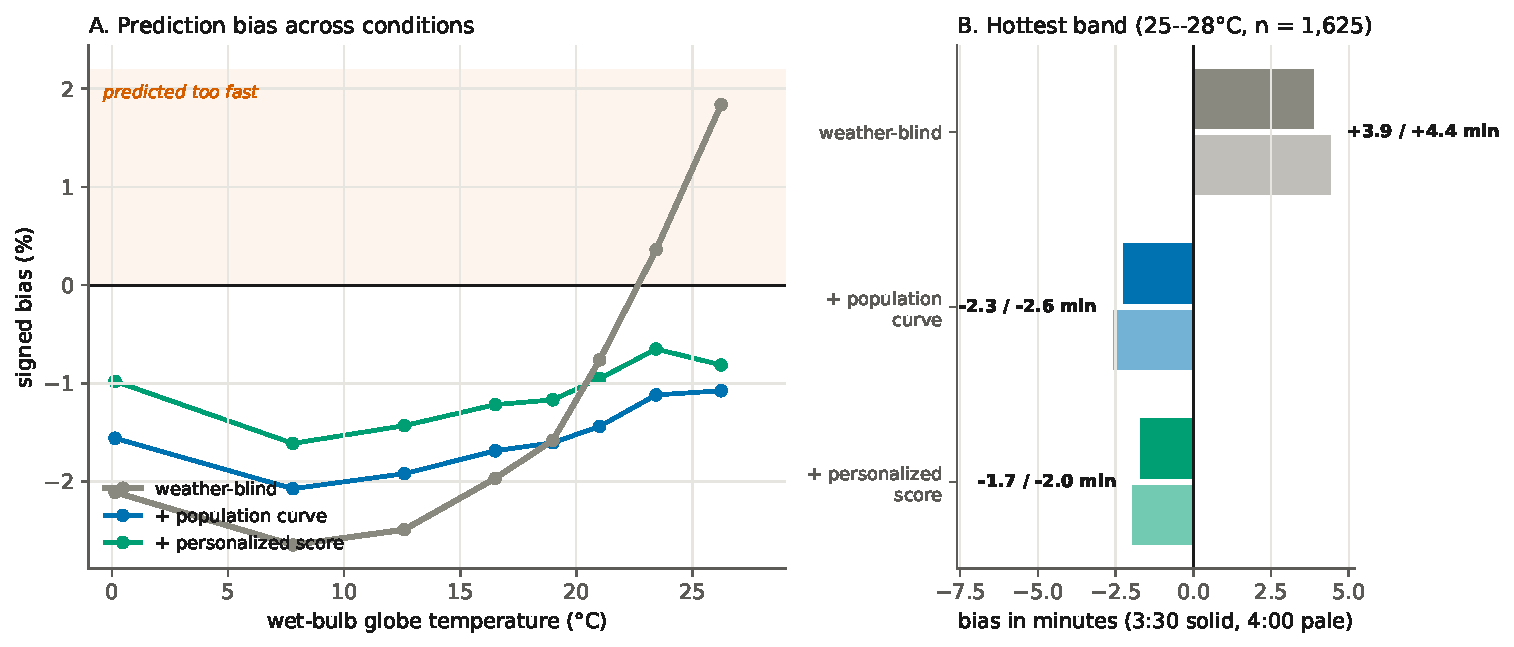
\includegraphics[width=\linewidth]{figures/fig_bias_fix.pdf}
  \caption{Prediction bias by wet-bulb globe temperature on the held-out set, where a positive value means a run was predicted faster than it was actually run. Panel A: the weather-blind model crosses into optimistic prediction in the hottest band, while both heat-aware models remain conservative throughout. Panel B: the same hottest band expressed as finish time for a 3:30 marathon.}
  \label{fig:bias_fix}
\end{figure}

\begin{figure}[!ht]
  \centering
    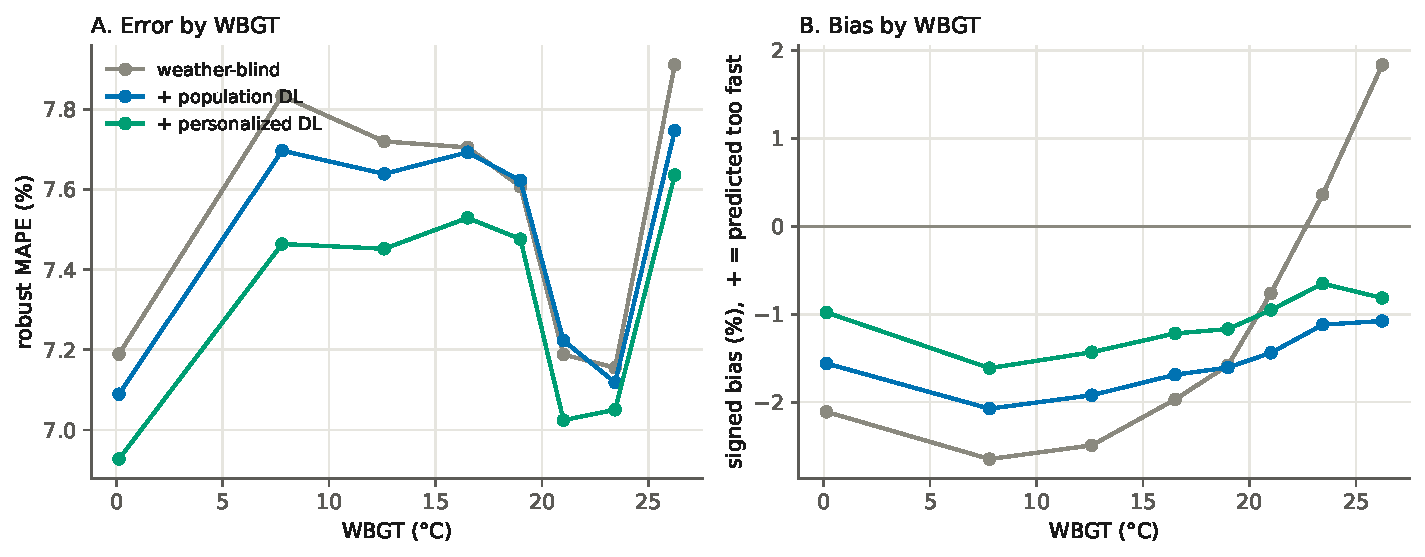
\includegraphics[width=\linewidth]{figures/fig_error_by_temp.pdf}
  \caption{Held-out error stratified by WBGT. Panel A: robust MAPE by WBGT bin for the three models; the personalized model is lowest in every bin. Panel B: signed bias by WBGT bin, where positive means predicted too fast. The weather-blind model swings from too slow in the cold to too fast in the hottest bin; the personalized model is closest to zero in most bins, with a curve nearly parallel to the population model's.}
  \label{fig:error_by_temp}
\end{figure}

\subsection{What the personalized score measures}

The personalized score improves prediction and depends on being matched to the right runner, but three diagnostics indicate that it is not a measure of heat sensitivity alone.

Its effect is nearly independent of temperature. Relative to the population model it shifts predictions by about $-0.2$ to $-0.5\%$ in every temperature band, and the row-level correlation between that shift and WBGT is $+0.026$. The shift is instead ordered by the runner's score quintile, which is why the bias curves in Figure~\ref{fig:bias_fix} run parallel.

Forcing it to act through the temperature curve retains only part of its value. Supplied as a percentile-matched deviation of the curve, so that its input is zero at and below the $10\,^{\circ}$C anchor, it yields 7.40\% robust MAPE, a gain of 0.098 points beyond the population curve with a 95\% interval of [0.041, 0.154]. That is a genuine temperature-shaped signal, but it is about 58\% of the 0.168-point gain the unconstrained score achieves. The remainder is runner-level information that is not specific to heat.

Calibrating both features against the correction the weather-blind model requires is best read as a sensitivity test rather than as a measurement, because the result depends on the specification. Fitted on the manuscript's baseline, the population curve's scale is $\alpha = 1.10$, with a 95\% interval of [0.91, 1.30] that includes one, so the magnitude the deep model learned agrees with the correction the pace model independently requires. The personalized deviation's coefficient is $\gamma = -0.96$ [$-1.71$, $-0.10$], negative: conditional on the population curve, runners the model marks as more heat-sensitive would require their predictions adjusted in the opposite direction.

Refitting that calibration while varying only how much runner-level information the baseline carries shows the coefficient is a property of the specification. With no runner-level features at all, $\gamma = -5.82$ [$-7.81$, $-3.88$]. With the manuscript's baseline, $-1.17$ [$-1.95$, $-0.39$] in this replication. Adding runner fixed effects to the calibration moves it to $+0.61$ [$-0.01$, $1.46$], and a per-runner intercept estimated from each runner's earlier activities gives $+0.15$ [$-0.27$, $0.73$]. Both intervals include zero. The population scale $\alpha$ moves along the same ladder in the same direction, from 3.31 with no runner-level information to 1.05 with the manuscript's baseline and 0.56 with the per-runner intercept, which is the population term absorbing the same runner-level confound before it is controlled.

The mechanism is a confound between runner identity and training climate. Across fitting runners, a runner's mean prediction error correlates with the wet-bulb globe temperature they habitually train in at $r = +0.19$, a slope of $+0.18$ percentage points per \textdegree C; the hottest habitual quartile carries a mean error of $+2.68$ points against $+0.80$ for the coolest. Any runner-level term therefore absorbs part of the heat signal without being shown a temperature, and a personalized heat feature estimated alongside one is left explaining a residual whose sign is not stable. Once runner identity is supplied directly, the personalized deviation adds nothing, which is the cleanest statement of what it was carrying.

\subsection{Benchmarking against the published forms}
\label{sec:benchmark}

Section~\ref{sec:literature} collected a dozen published heat corrections. Because each can be written
as a multiplicative adjustment to a weather-blind prediction, all of them can be dropped into the same
slot as the learned curve and scored on identical held-out runs. Each form is evaluated on the
temperature variable it was fitted on and centered on the fitting sample, so what is compared is its
shape and magnitude rather than its arbitrary reference point.

\begin{table}[!ht]
\centering\small
\caption{Held-out bias by heat threshold, out-of-fold over the 2{,}143 runners with an estimable
heat tolerance (400{,}337 runs). Flatness is the root-mean-square variation of the bias profile across
WBGT bins; lower means less of the error is predictable from conditions.}
\label{tab:benchmark}
\begin{tabular}{@{}lrrrrr@{}}
\toprule
& \multicolumn{4}{c}{signed bias (\%)} & \\
\cmidrule(lr){2-5}
Correction & 15+ & 20+ & 23+ & 25+ & Flatness \\
\midrule
None (weather-blind)          & $+0.10$ & $+0.94$ & $+1.63$ & $+2.08$ & 1.19 \\
\textbf{This study}           & $-0.58$ & $-0.52$ & $-0.46$ & $-0.47$ & \textbf{0.10} \\
Martin 1999                   & $-0.57$ & $-0.73$ & $-0.69$ & $-0.71$ & 0.29 \\
Mantzios 2022 (marathon)      & $-0.46$ & $-0.19$ & $+0.17$ & $+0.41$ & 0.40 \\
Ely 2007 (25th place)         & $-0.95$ & $-0.73$ & $-0.41$ & $-0.18$ & 0.49 \\
Guy 2014                      & $-0.83$ & $-0.48$ & $\mathbf{-0.03}$ & $+0.34$ & 0.58 \\
Vernon 2021 (mass field)      & $-2.64$ & $-3.40$ & $-3.53$ & $-3.62$ & 2.13 \\
\bottomrule
\end{tabular}
\end{table}

Three things follow. The learned curve is the flattest of the corrections by a wide margin: its
residual bias sits between $-0.46$ and $-0.58\%$ at every threshold, a root-mean-square variation of
0.10 against 0.29 for the next best form, so almost none of what remains is predictable from
conditions. What remains is a small uniform over-correction, and the form whose residual comes nearest
zero in the hottest strata, Guy's capped slope, does so by crossing from under- to over-correction as
the threshold rises rather than by being flat. The learned curve is also the only form whose published magnitude needs essentially no rescaling
on training runs; fitting a free scale to it returns $1.09$, against 0.77--0.79 for Ely's and Guy's
elite forms and 1.46 for Mantzios's marathon slope. Forms estimated on mass fields over-correct severely when applied to training runs, by
factors of three to fourteen (the Gasparetto quadratics by more than an order of magnitude and are
omitted from the table), which is the expected direction given that race-day heat sensitivity exceeds
training-pace sensitivity, by the factor of about five measured in Section~\ref{sec:raceday}. And the elite forms, which are shallower, transfer well: Martin's quadratic
is the next flattest, though it achieves this partly by bending in cool conditions where the learned
curve is deliberately flat.

Figure~\ref{fig:litbench} shows the same comparison as a profile. No published form and no fitted
correction alters mean absolute error appreciably, all but the mass-field Vernon form (7.74\%) sitting between 7.42\% and 7.48\% on this sample; a three-percent effect is not visible against day-to-day variation in a per-run error statistic,
which is why calibration rather than error is the reported criterion throughout.

\begin{figure}[!ht]
\centering
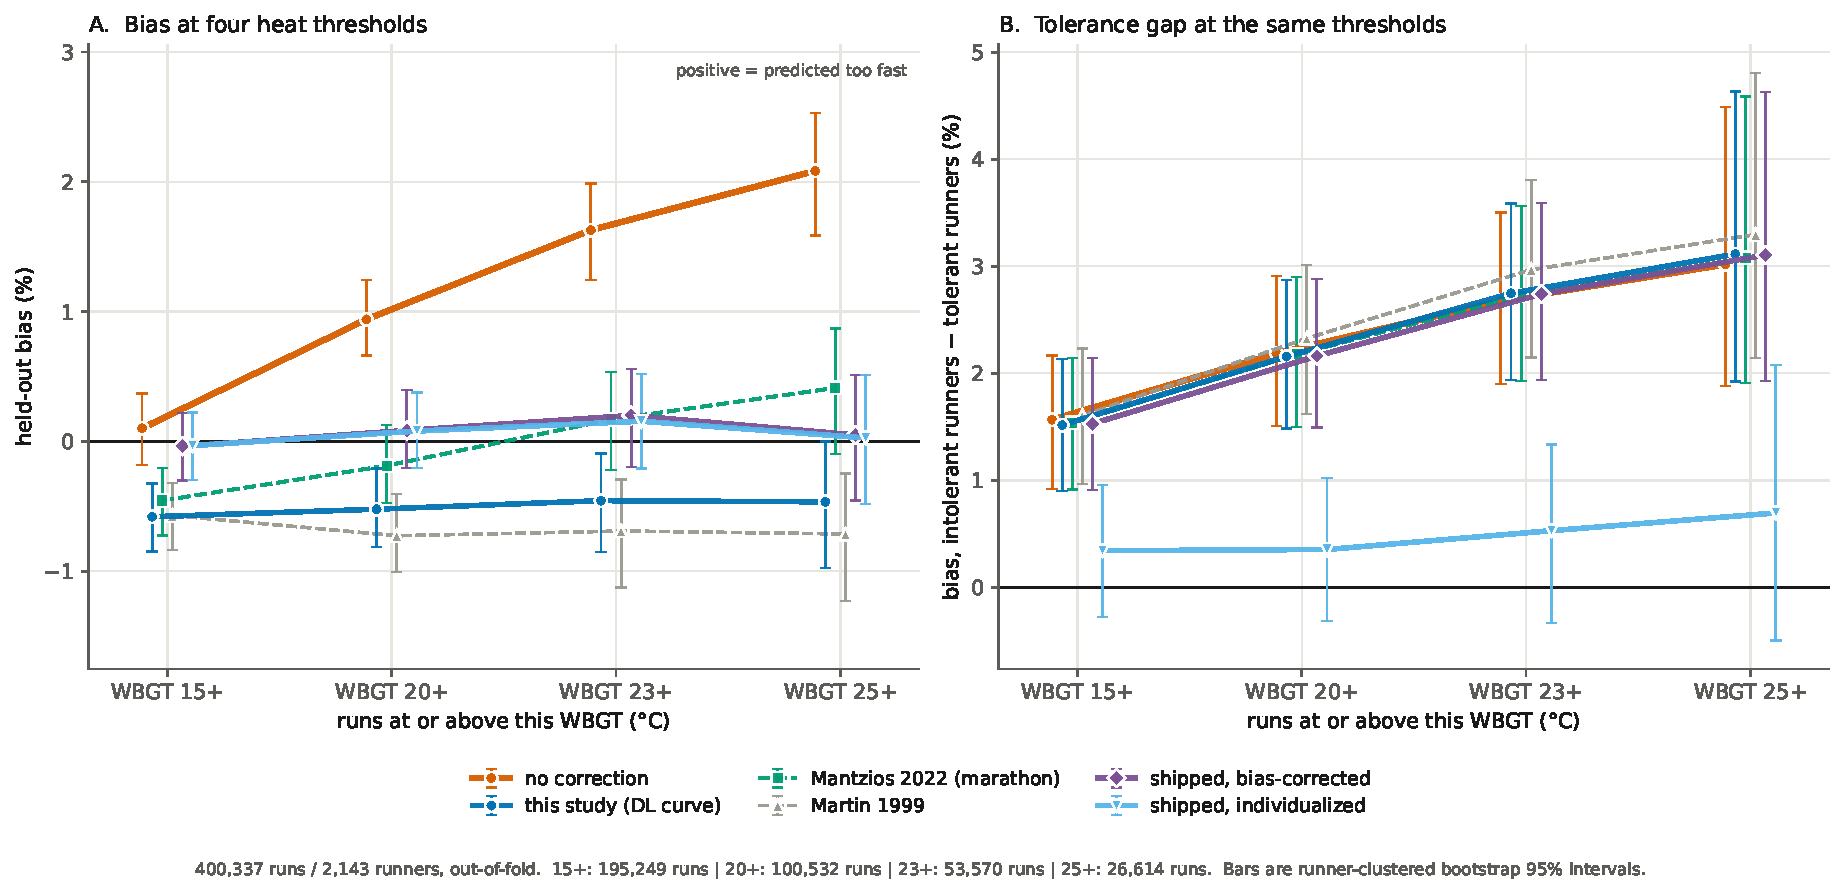
\includegraphics[width=\linewidth]{figures/fig_lit_benchmark.pdf}
\caption{Held-out bias (left) and the same models' bias among heat-intolerant versus heat-tolerant
runners (right), at four cumulative WBGT thresholds. Bars are runner-clustered bootstrap 95\%
intervals. The two series labelled ``shipped'' are the deployed adjustment layer: the population curve after an affine, out-of-fold calibration, and the same with each runner's heart-rate-derived heat-tolerance estimate applied (Section~\ref{sec:future}). A correction that has removed the conditions-dependence sits flat near zero across all four
thresholds rather than crossing it once.}
\label{fig:litbench}
\end{figure}

\subsection{Robustness to the choice of baseline}

Because that reversal is conditional on a baseline containing heart rate, the whole progression was repeated on a baseline that removes current effort entirely, using an independently trained marathon-fitness estimate with distance and elevation. This branch is supplementary and is not an equivalent comparison, since it changes the fitness representation and drops current effort at the same time, which raises its absolute error; the fixed fitness estimate is also available for only two thirds of the enlarged corpus, so the branch runs on 16{,}554 held-out activities from 103 runners. Within it, the population temperature information remains useful though its gain interval includes zero (0.09 points [$-0.10$, 0.25]), raw WBGT produces a gain of the same size, and the strict-prior personalization's gain over the population curve, 0.16 points [$-0.03$, 0.38], no longer excludes zero. The $\gamma$ reversal disappears ($\gamma = +1.12$ [$-0.92$, 3.31]), but the estimate is imprecise and unstable across runner folds. A narrower ablation that keeps the trailing-pace fitness proxy and removes only current heart rate gives the same picture with more precision: the population curve improves on the blind baseline by 0.03 points [0.01, 0.06], the personalized score by a further 0.09 [0.01, 0.18], and the shuffled control by 0.01 [$-0.01$, 0.03]. The result is that the personalized finding depends on the conditional baseline, and that this branch neither confirms nor refutes its magnitude.

\subsection{Acclimation}


The literature in Section~\ref{sec:literature} predicts that recent heat exposure should reduce a runner's heat penalty. Two tests examine whether the model's per-runner score behaves that way.

The first compares the score against each runner's recent training conditions. For every activity the number of runs above $18\,^{\circ}$C WBGT in the preceding fourteen days is counted, and the runner's prospective sensitivity rank is regressed on it within runner, with the current run's WBGT as a control and a placebo term for the fourteen days that follow. One standard deviation more recent hot training lowers the rank by 0.94 percentile points (runner-clustered 95\% interval [$-1.23$, $-0.64$]), which is the direction acclimation predicts, while the same count over the following fourteen days has no effect ($+0.08$ [$-0.19$, 0.34]), so the association is not a season or climate artifact. An exposure measure that decays with a fourteen-day half-life gives the same answer ($-0.73$ per standard deviation [$-1.13$, $-0.33$]). Across within-runner deciles of exposure the rank falls almost monotonically (every step after the second decile is downward), from $+0.9$ points in the least-exposed decile to $-1.6$ in the most exposed.

The second test uses an independently curated set of candidate acclimation episodes: pairs of hot runs, matched on conditions, recorded before and after a block of heat exposure, with a control set of pairs that bracket no such block. Across 465 low-to-high exposure episodes from 353 runners, performance in matched conditions improves after the block by 1.95\% [1.34, 2.56], and 63\% of episodes improve; across 450 low-to-low control episodes from 359 runners the improvement is 0.55\% [$-0.03$, 1.13]. The difference, 1.40 percentage points [0.54, 2.27], is the acclimation effect the design isolates.

Both tests are consistent with acclimation, and neither is decisive. The episodes are candidates identified from training history rather than verified physiological measurements, and few runners contribute repeated episodes above $25\,^{\circ}$C (29 episodes from 24 runners), so no individual adaptation magnitude can be estimated. What the corpus supports is that acclimation is detectable as a population-level tendency in these data, and that the model's per-runner score moves with it in the expected direction. What it does not support is a per-runner acclimation state that could be tracked over a training block, which would require either denser sampling in heat or the physiological markers, resting heart rate chief among them, that consumer devices do not reliably record.

\subsection{The race-day scale of the curve}
\label{sec:raceday}

The within-person edition effects estimated from official results (Section~\ref{sec:raceday_methods}) track the learned curve (Figure~\ref{fig:raceday}). With course and calendar-year fixed effects the scale is $\alpha = 4.9$ [3.4, 6.5] ($R^2 = 0.71$ across the 49 editions); with course effects only it is 4.85 [3.28, 6.41], and an unweighted fit gives 5.2 [3.3, 7.2]. The hottest editions anchor the estimate: New York City 2022 (race-window WBGT 21.1\,\textdegree C) ran 4.9\% slower than that course's mean edition, Chicago 2021 (20.1\,\textdegree C) 3.4\% slower and London 2018 (17.9\,\textdegree C) 5.8\% slower, against training-run curve values of 1.3, 1.1 and 0.6\%. The calendar-year effects are themselves informative: within person, 2019--2025 editions are about one percentage point faster than 2015--2018, consistent with the change in racing shoes over that period, and omitting them makes cool recent editions look anomalously fast.

The same scale appears inside the corpus. On labelled marathon efforts identified from the runners' own activity records, the curve's fitted scale is 6.0 [3.9, 8.5] on the strictest label set ($n = 625$) and 4.7 [2.9, 6.6] on all band-eligible efforts; on labelled half marathons it is 3.7 [2.5, 4.9]; on training runs it is 1.00 [0.87, 1.15]. The training-run curve is therefore the right shape at the wrong scale for a race, and the factor is about five for a marathon, lower for a half.

Nothing else in the race-day weather adds to the curve at the edition level. Fitting a physics-form wind-drag term alongside the curve, from hourly wind projected on each course line, gives a coefficient of $-0.00$ [$-0.56$, 0.56] with year effects and 0.20 [$-0.27$, 0.66] without, against a value near 2 that unsheltered drag physics would imply; it is null separately on the loop courses and on the point-to-point courses (Boston and Big Sur). A LASSO over thirteen race-day components with the curve unpenalised selects dew point, solar radiation and the rise in WBGT during the race window, each worth 0.3 to 0.7\% per standard deviation, and none of wind speed, gusts, headwind, precipitation, cloud or pressure. On the corpus's training runs the drag coefficient is measurable but small, 0.25 [0.12, 0.38], about one eighth of the unsheltered value (Section~\ref{sec:future}).

\begin{figure}[!ht]
  \centering
  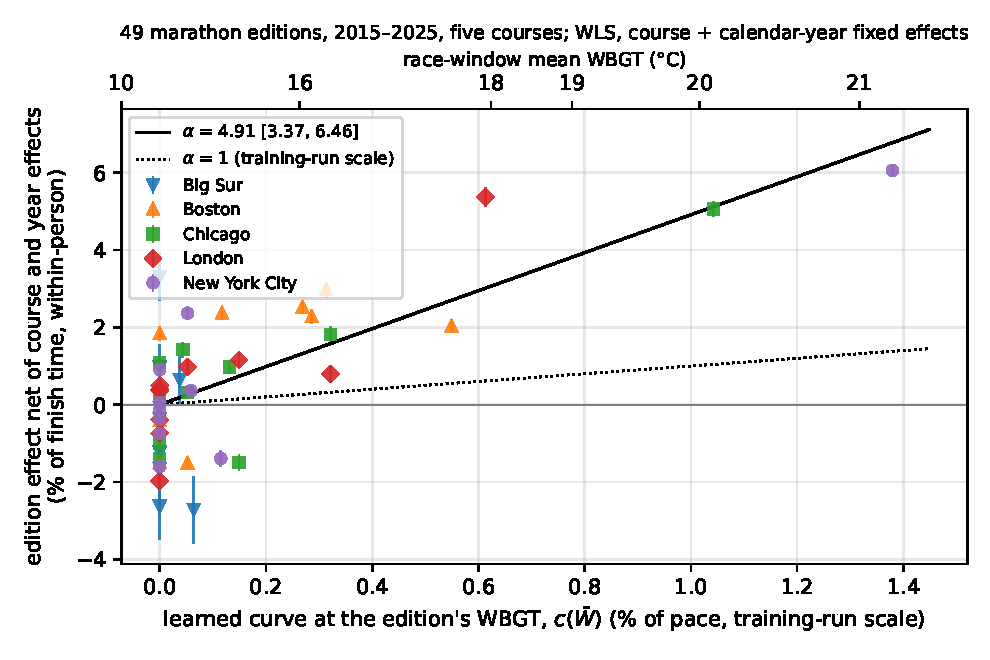
\includegraphics[width=0.9\linewidth]{figures/fig_raceday_scale.pdf}
  \caption{Within-person edition effects from official results against the learned curve evaluated at each edition's race-window WBGT. Points are edition effects net of course and calendar-year fixed effects, with 95\% intervals from person-clustered standard errors; the solid line is the fitted scale $\alpha$ and the dotted line the training-run scale $\alpha = 1$. 49 editions of five marathons, 2015--2025.}
  \label{fig:raceday}
\end{figure}

\section{Discussion}
\label{sec:discussion}

\subsection{Implications}

Literature on heat's effect on endurance running and prediction modeling have developed separately. Research quantifying heat effects is retrospective: it regresses observed finishing times on the conditions those races happened to be run in on a field-wide level. Predictive running models, including those shipped with consumer running platforms, work from training history and take no account of race-day conditions. This paper joins the two: it predicts pace for a run that has not yet taken place based on that runner's prior training and forecasted conditions. In doing so, it becomes the first prospective, individual-level pace prediction to incorporate a heat response.

The population curve that results is well scaled rather than merely correlated with conditions. On training runs its calibration coefficient is compatible with one, meaning the magnitude the deep model learned matches the correction the pace model independently requires; on official race results the same shape applies at 4.9 times that scale, which places it inside the band of published mass-field forms once the training-to-race factor is accounted for. Its most consequential property is directional. A weather-blind model predicts runs in the hottest conditions faster than they were actually run, and supplying the curve removes that optimism. Because the error such a model makes is systematically in the runner's disfavor on precisely the days when conditions matter most, correcting its direction is worth more than the small reduction in average error suggests. The magnitude is quantifiable. At training-run scale the curve implies roughly nine additional minutes at $28\,^{\circ}$C for a runner whose ideal-weather marathon prediction is 3:30 and ten for a four-hour runner; at the race-day scale of Section~\ref{sec:raceday} a marathon at 21\,\textdegree C WBGT costs about 6.5\% of finish time, or fourteen minutes for the 3:30 runner, and 28\,\textdegree C would cost over 20\%, though no edition in the validation set reached that far.

The per-runner result is more equivocal. A score matched to the correct runner improves prediction reproducibly, and shuffling that match removes the gain, so the score carries genuine individual information. Part of its effect is temperature-shaped: forced to act only through the temperature curve, as a percentile-matched deviation that is zero at and below the $10\,^{\circ}$C anchor, it retains 58\% of the unconstrained gain, so a runner scored as more sensitive does require a progressively slower prediction as conditions worsen; the remainder is a runner-level shift that does not vary with temperature. What does not survive is conditioning: the residual direction inverts once heart rate enters the baseline. A linear replication of the calibration makes the dependence on the conditioning set explicit: with heart rate in the baseline the personalized deviation's coefficient is $+0.24$ per unit [$-0.69$, 1.17] under linear controls and $-0.95$ [$-1.89$, 0.01] under spline controls, neither distinguishable from zero, whereas with current heart rate removed it is $+0.87$ [0.16, 1.58] under linear controls and $-0.21$ [$-0.93$, 0.53] under spline controls; the sign is not stable across estimators once heart rate is removed either, so the reversal is a property of the conditioning set and the estimator together rather than of the score alone. Both results are what would be expected if heat sensitivity were already partly expressed through the physiological signals the baseline observes, in which case the personalized feature absorbs what remains rather than the effect itself. Replacing the population curve by each runner's own curve, without a separate rank, is consistent with that reading: error is essentially unchanged (7.50\% for the substituted curve against 7.50\% for the population curve alone, and 7.56\% with no heat term at all) and the bias moves in the physiologically expected direction ($-1.31\%$ against $-1.64\%$), but the gain that the separate rank supplies (7.33\%) does not appear, which is the signature of runner-level rather than heat-specific information. Separating a runner's heat sensitivity from its own downstream consequences therefore requires either a baseline that excludes those consequences or measurements that identify them directly, and the sensitivity analysis reported above shows that the first is not sufficient on its own.

\subsection{Who is in this corpus, and which way that biases the estimate}
\label{sec:selection}

The corpus is not a sample of runners, and it is not a sample of races. It is a sample of training runs
recorded by people who chose to wear a GPS watch and to share the data with a fitness platform. Three
selection mechanisms follow, and each has a predictable direction, summarized in
Table~\ref{tab:selection}.

Runs are overwhelmingly training rather than racing. A runner who is not competing can slow down,
shorten, reschedule to a cooler hour, or move indoors when conditions are bad, and all four responses
either remove the observation or blunt it. The effect estimated here is therefore the effect on a runner
free to concede, which is a lower bound on the effect at a race, where the runner is not.

The people are self-selected toward commitment. Opting into a training platform, wearing a monitor
consistently, and accumulating the thirty-activity history the model requires all select for volume and
consistency, and plausibly for fitness and heat acclimatization. More acclimatized runners are less
heat-sensitive, so this too biases the population curve downward.

And within a runner, hot days are not randomly assigned to sessions. Hot runs in this corpus are
slightly shorter (within runner, about 0.2\,km less per 10\,\textdegree C of WBGT), though not measurably easier by relative heart rate. Since the penalty is steeper at high effort
(Section~\ref{sec:results}), conditioning on the runs that actually happened understates what heat would
have cost had the same session been attempted regardless.

\begin{table}[!ht]
\centering\small
\caption{Selection mechanisms and the direction each pushes the estimated heat effect.}
\label{tab:selection}
\begin{tabular}{@{}p{5.2cm}p{4.8cm}p{3.2cm}@{}}
\toprule
Mechanism & Why it operates & Expected sign \\
\midrule
Training runs, not races & the runner may slow, shorten or reschedule & \textbf{understates} \\
Platform opt-in, 30-run history requirement & selects committed, higher-volume, likely more acclimatized runners & \textbf{understates} \\
Hot sessions are shorter & less of the session is run in the binding regime & \textbf{understates} \\
Runs abandoned on the worst days & the observation is never recorded & \textbf{understates} \\
Warm-climate runners supply most hot runs & they are the most acclimatized & \textbf{understates} \\
\bottomrule
\end{tabular}
\end{table}

The mechanisms point the same way, which is convenient for interpretation if uncomfortable for
precision: the population curve should be read as a floor on race-day cost rather than an unbiased
estimate of it. Section~\ref{sec:raceday} puts a number on that floor: race-day finish times follow the
same curve at about five times the scale, which is consistent with Section~\ref{sec:benchmark}, where forms
fitted on actual mass-participation races imply substantially steeper slopes than the one learned here. It is also why no
attempt is made to extrapolate to championship conditions: this corpus cannot speak to a runner who has
no option to concede.

\subsection{Limitations}

The primary caveat is that this is a runner-disjoint held-out prediction, not a formal causal estimate of heat's physiological effect. The corpus is training runs, where improvements are calibration and accuracy gains on held-out training run pace rather than measured heat responses. The official results of Section~\ref{sec:raceday} supply the race-day scale, but at the level of whole editions rather than of individual runners: they show that the population curve is the right shape for race day and how much steeper it is there, not whether an individual's sensitivity transfers. A per-runner race-day test would need the training histories and the race results of the same people, which the linkage does not yet provide at scale. The headline amplitude also moved during training: the median penalty at $28\,^{\circ}$C was 4.8\% at one million steps and 4.2\% at the reported checkpoint, a change of about twelve percent while the shape of the curve held, so the reported magnitude carries a training-length uncertainty of that order on top of its sampling interval.

Second, runs at the extreme hot end are sparse. The held-out cohort is bounded above at $28\,^{\circ}$C by the ceiling imposed in Section~\ref{sec:methods} based on sparsity; the enlarged corpus more than doubled the runs above that point, which is what made the ceiling supportable at 28 rather than 25\,\textdegree C. Even below it, the warm bins hold fewer activities than the mild ones (1{,}625 held-out activities between 25 and $28\,^{\circ}$C against 5{,}398 between 10 and 15), leading to the hot-end estimates carrying the most sampling uncertainty. Denser sampling of genuinely hot runs would tighten these estimates.

Third, the per-runner result is narrower than it first appears. The score carries genuine individual information, since matching it to the correct runner improves held-out prediction and scrambling the assignment removes the gain. But the diagnostics in Section~\ref{sec:results} show that information is not heat sensitivity specifically: the effect is roughly constant across temperature, only about 58\% survives when constrained to act through the temperature curve, and the direct calibration returns the wrong sign. Either the baseline's heart rate has already slowed heat-sensitive runners on the same evidence, leaving the score to push back against a correction already made, or the deep model has the ordering wrong. Removing heart rate eliminates the reversal, favoring the first explanation, but too imprecisely to settle it. Until a baseline exists in which it is clear what each feature stands in for, the score is usable as evidence that a runner tends to be over- or under-predicted, not as a measurement of how much heat costs them.

Finally, some of what the literature flags as relevant is simply absent from the data. Raw GPX files carry no body mass, though heat production scales with it and smaller runners are advantaged in heat \citep{marino2008, maughan2010}; no biological sex, an established performance differential under heat \citep{llewellyn2025, vihma2010, kelly2023, weiss2022b}; and no resting heart rate, one of the most validated acclimation markers \citep{periard2015, tyler2016, pryor2019}. Each would plausibly improve prediction. Laboratory variables such as plasma volume or sweat sodium concentration are further out of reach, since they cannot be obtained from consumer devices at all.

\subsection{Future extensions}
\label{sec:future}

Several extensions follow from the results above; each is stated with the evidence that motivates it and the form it should take, so that they can be built without relitigating the design.

\emph{A physics-form wind term with a calibrated coefficient.} Aerodynamic drag scales with the square of air speed, so the extra cost of wind on a course segment with along-path headwind $H$ is proportional to $(v+H)^2 - v^2 = 2vH + H^2$, averaged over the runner's route and race hours; on a loop the linear term cancels while the quadratic does not, and on a point-to-point course the linear term dominates and changes sign with the wind. Estimated on 330{,}000 corpus runs with 30-second GPS bearings, within runner and after the heat curve, the coefficient on this term is 0.25 [0.12, 0.38] in percent of pace per unit of relative drag work, against a value near 2 that unsheltered physics would imply for a runner at three metres per second; the edition-level estimate is 0.20 [$-0.27$, 0.66]. Mass fields shelter and draft, and reanalysis wind is a coarse measure of what a runner meets at street level, so the empirical coefficient is the one to use. At that coefficient a strong headwind on a point-to-point course costs about one percent and wind on a loop course a fraction of that, so the term belongs in a calculator as the one-parameter formula above rather than as a learned model: an earlier attempt to give the transformer a headwind channel degraded its fitness reconstruction, and there is under one percent of pace to recover.

\emph{Course terms from same-person official results.} The person linkage yields 448{,}000 cross-course pairs, and the same-person course effects they identify differ from what terrain alone predicts: relative to Chicago, and net of each edition's conditions, New York City costs $+2.5\%$ (standard error 0.04), London $+2.1\%$, Boston $+1.2\%$ and Big Sur $+5.4\%$, whereas a grade-adjusted cost of each course's measured elevation profile gives $+0.6$, $-0.0$, $-0.2$ and $+1.5$ percentage points. The remainder is what terrain does not carry: turns, bridges, crowding and how a course is raced. A hierarchical course model with the terrain term as its prior mean, fitted to these pairs, is the natural next component of a race-day predictor; extending the crawl to the remaining large marathons and half marathons is in progress.

\emph{Distance-specific race scales.} After the heat curve is applied, the within-runner residual is $-0.6\%$ on hot runs under 8\,km and $+1.3$ to $+1.4\%$ on hot runs of 18\,km and longer, so a single curve averaged over mostly short training runs over-corrects short efforts and under-corrects long ones. The labelled-race scales of Section~\ref{sec:raceday} (3.7 for halves, about five for marathons) are one expression of the same gradient. A predictor should carry the scale as a function of distance rather than as one number.

\emph{Time-resolved conditions.} The rise in WBGT during the race window is selected by the LASSO at edition level and is significant within runner on the corpus ($+0.2\%$ per standard deviation), as is solar radiation beyond what WBGT carries. Both argue for evaluating the curve on the conditions a runner meets over their own hours on the course rather than at the gun, which a forecast permits directly.

\emph{Acclimation as a deviation from training climate.} Within runner, each degree by which a run's WBGT exceeds the runner's trailing 60-day training WBGT costs about 0.22\% of pace (positive deviations only; negative deviations cost nothing), which is the pace-side signature of the acclimation that Section~\ref{sec:results} detects. The term should not be stacked on the population curve, which already reflects runners at their usual acclimation and over-corrects when both are applied; its use is the climate-move case, where a runner races somewhere hotter than they trained, and the recovery curve after arrival.

\emph{Per-runner tolerance from heart rate.} The per-runner score from the transformer is not separable from fitness (Section~\ref{sec:discussion}). A runner's heart-rate response to heat at matched load is more reliable (split-half 0.47, rising with history length) and is not confounded with fitness (correlation with the fitness estimate near zero). Applied out of fold as a scaling of the population curve, it removes most of the residual hot-day bias between heat-tolerant and heat-sensitive runners, but its precision supports only three to five tiers, not a percentile; that is the form in which personalization should ship.

\emph{Calibration of the training-run curve under a physiological baseline.} In the paper's own harness with heart rate in the baseline, the curve over-corrects within runner by about a quarter (residual slope on the curve $-0.23 \pm 0.05$), and a small cold cost of about $+0.3\%$ remains below 4\,\textdegree C where the curve is flat. Both are second-order relative to the race-day scale but should be folded into any deployed calibration.

\clearpage
% The style is set once in the preamble (\bibliographystyle{plainnat}). A second
% \bibliographystyle{apalike} stood here and was inert: BibTeX takes the first
% and reports "Illegal, another \bibstyle command" for the second, so the paper
% has always rendered as plainnat. Removing it keeps the output identical and
% clears the error. To actually switch to apalike, change the preamble line.
\bibliography{references,tommy_refs}
\clearpage
%% create appendix
\appendix
\renewcommand{\thetable}{A\arabic{table}}
\setcounter{table}{0} % This resets the table counter
\renewcommand{\thefigure}{A\arabic{figure}}
\setcounter{figure}{0}
\section{Model and Training Specification}
\label{app:model}

This appendix states the deep-learning model in full. Section~\ref{sec:methods} describes what the
model is for; what follows is what it is.

\subsection{Input representation}

One training example is a window of a single runner's $T = 30$ most recent activities, ordered in
time, with the activity to be predicted last. Each activity is resampled to $R = 128$ points spaced
equally in distance rather than in time, so that a point index refers to the same fraction of the
run regardless of its duration. An example is therefore a tensor
\begin{equation}
  X \in \mathbb{R}^{T \times R \times C}, \qquad T = 30,\; R = 128,\; C = 11,
\end{equation}
with channels in fixed order: date, latitude, altitude, cadence, cumulative elevation, distance,
heart rate, power, activity type, outdoor WBGT, and pace. Pace occupies the final index by
construction, since the loss and the readout both address the target channel positionally.

Runners with fewer than 30 recorded activities are retained by padding the window at the front. Pad
slots are exactly zero in every channel, and a per-activity key mask excludes them from
cross-activity attention, so a short history is treated as short rather than as a sequence of
zero-valued runs. Establishing that contract required care: the date channel is centered by
subtracting the window maximum, which is applied after padding and would otherwise leave pad slots
with a nonzero date and defeat the mask. The centering is therefore recorded before the shift and
the pad slots reset after it.

Two channels are masked on the target activity only: pace, which is the prediction target, and
power, which is close to a deterministic function of pace and would otherwise leak it. Both remain
visible on all preceding activities. Weather channels are never masked, since race-day conditions
are known in advance from a forecast at the moment a prediction would be used.

Pace is smoothed along the distance axis with a trailing 10-point moving average. A centered filter
was used initially and is wrong for this purpose: zero-padding at the window edges biases the first
and last points toward zero, which reports the end of a run as faster than it was. Since the late
stages of a hot run are where the effect under study appears, the label was biased against the
hypothesis. The trailing filter costs a phase lag of roughly five points, uniform across all runs
and therefore incapable of confounding a weather comparison.

\subsection{Tokenization and embedding}

Every channel is discretized and embedded rather than consumed as a real number. Channel $c$ carries
a fixed edge vector $e^{(c)}$, and a value $v$ maps to the token index $\mathrm{digitize}(v,
e^{(c)})$, which indexes a learned table $E^{(c)} \in \mathbb{R}^{B_c \times d}$ with $d = 64$. Edges
are fixed at initialization: the index enters an integer lookup, so no gradient reaches the edges
and their placement is a design choice rather than a learned quantity.

Most channels use $B_c = 500$ bins. Placement is per-channel. Sensor channels use quantile edges;
pace uses uniform edges over $[0, 40]\,\mathrm{min\,km^{-1}}$, which matters because the loss reads
its bin grid from the pace row and uniform spacing makes that grid a linear pace axis. WBGT uses 100
quantile edges. The asymmetry is deliberate. For sensor channels, quantile placement concentrates
resolution in the dense middle and starves the sparse tails, where long runs and hard efforts carry
the fitness signal; substituting quantile edges for sensors cost 0.07 in $R^2$ in a direct test. For
WBGT the binding constraint is the number of hot runs available, which no bin placement can change,
so placing 100 bins where the observations actually are is the better use of them.

An absent sensor is a distinct token rather than a zero. Heart rate and power are frequently missing,
and mapping a missing reading to zero collides with a genuine reading of zero. Missing values survive
tokenization as \texttt{NaN} and map to index $B_c$, an extra row in the embedding table.

The channel embeddings at each point are summed and scaled, then combined with learned positional
embeddings over both axes and layer-normalized:
\begin{equation}
  z_{t,r} \;=\; \mathrm{LayerNorm}\!\left(\frac{1}{\sqrt{C}}\sum_{c=1}^{C} E^{(c)}\!\left[k^{(c)}_{t,r}\right]
                \;+\; P^{\mathrm{act}}_{t} \;+\; P^{\mathrm{pt}}_{r}\right).
\end{equation}
The $1/\sqrt{C}$ scale and the normalization are not cosmetic. A plain sum has standard deviation
growing as $\sqrt{C}$, which overwhelms the fixed-scale positional term and destabilizes the first
pre-normalization block. Introducing both raised held-out $R^2$ from 0.673 to 0.710 and lowered
error from 6.99\% to 6.60\% at a cost of 128 parameters.

\subsection{Factored attention}

Attention is factored over the two axes instead of applied to the flattened $T \times R = 3{,}840$
sequence, whose quadratic cost would be prohibitive. Each of the $L = 5$ layers applies attention
within an activity, across the $R$ points, and then attention across activities at matched point
index. The within-activity pass reads the shape of a single run; the cross-activity pass is where a
runner's recent training history, and therefore the fitness estimate and any conditioning context,
is assembled. The cross-activity block uses a low-rank projection, and the padding mask enters here
as a key mask so that padded slots cannot be attended.

Attention is bidirectional. No causal mask is applied along the point axis, since the whole of each
preceding activity is legitimately available and only the target activity's pace is withheld.

Hyperparameters: $L = 5$ layers, 8 heads, feed-forward width 256, embedding width 64, dropout 0.1.
Total parameters 5{,}950{,}251.

\subsection{Objective}

The model does not regress pace. It predicts a distribution over the 500 pace bins at each point and
is trained by cross-entropy against the bin containing the observed pace,
\begin{equation}
  \mathcal{L} \;=\; -\frac{1}{R}\sum_{r=1}^{R} \log \pi_{r}\!\left[\,b(y_{r})\,\right],
  \qquad b(y) = \mathrm{digitize}\!\left(y, e^{(\mathrm{pace})}\right),
\end{equation}
where $\pi_r$ is the predicted distribution at point $r$ of the target activity and $y_r$ the
observed pace there. The loss is computed on the target activity only.

A classification head over a continuous quantity is an unusual choice and is made for two reasons.
It imposes no parametric error distribution, so a skewed or multimodal pace at a given point is
representable; and it yields a predictive distribution at no extra cost, from which an interval
follows directly. Point predictions are read off as the expectation $\hat{y}_r = \sum_j \pi_{r,j}
m_j$ over bin midpoints $m_j$, and an activity-level prediction is the mean over the $R$ points.

Because the loss addresses the pace grid positionally, the bin edges must be stacked in numeric
channel order. Sorting them lexicographically, as a naive traversal of the parameter tree does,
places channel 9 after channel 10 and silently scores pace against another channel's grid. The
signature is diagnostic and worth recording: training loss falls normally while held-out error
remains pinned near 132\%, the value obtained by predicting the center of the bin range.

\subsection{Optimization}

Adam with global-norm gradient clipping at 1.0. The learning rate warms linearly from 0 to
$1\times10^{-4}$ over 1{,}000 steps, then follows a cosine decay to $1\times10^{-5}$ over 200{,}000
steps. Batch size 64, data-parallel across two GPUs. Training runs 200{,}000 steps, roughly 20 hours.

Checkpoints are written whenever held-out $R^2$ or error improves. These two criteria do not peak
together: $R^2$ peaks near 115{,}000 steps while error continues to improve to roughly 190{,}000.
Both checkpoints are therefore evaluated and reported, since selecting on $R^2$ alone overstates
error by about 0.2 percentage points. The artifacts in this paper come from the error-selected
checkpoint.

\section{Construction of the Heat Artifacts}
\label{app:curve}

Both heat artifacts are read off the trained model by counterfactual sweeps. For a runner's window,
the WBGT channel of the target activity is overwritten with a constant $w$ while every other channel
is held fixed, and the model is re-evaluated. The difference between two such evaluations is
attributable to WBGT alone, since nothing else in the input has changed. The sweep covers 5 to
30\,\textdegree C in 0.5\,\textdegree C steps; artifacts are truncated to $[10, 28]$, a 37-point
grid, because the evaluation panel contains no held-out target above 29.8\,\textdegree C and the
region beyond it cannot be checked.

Write $D_a(w)$ for runner $a$'s swept prediction. The runner's sensitivity is the percentage
slowdown at 28\,\textdegree C relative to 10\,\textdegree C,
\begin{equation}
  s_a \;=\; 100\left(\frac{D_a(28)}{D_a(10)} - 1\right),
\end{equation}
and the runner's normalized shape is $\phi_a(w) = \left(D_a(w)/D_a(10) - 1\right)\big/ (s_a/100)$,
which equals 0 at 10\,\textdegree C and 1 at 28\,\textdegree C by construction. Separating shape
from scale is what makes the median meaningful: runners differ mostly in the steepness of the
response, so averaging unnormalized curves would confound the two.

The population curve is $g(w) = \bar{s}\,\cdot\,\mathrm{med}_a\,\phi_a(w)$, the median shape rescaled
by the median sensitivity of the reference sample. The monotone projection $\max$-accumulate is
applied to the median shape at this point; as reported in Section~\ref{sec:methods} it moves 8 of 37
grid points by at most 0.13 percentage points.

A single window's sensitivity is dominated by noise, with test-retest reliability near 0.34, so
roughly three-quarters of the observed spread in $s_a$ across windows is measurement error rather
than a difference between runners. Averaging the 15 most recent windows raises reliability to
approximately 0.8. The per-runner score is therefore the percentile rank of a runner's window-averaged
sensitivity against the distribution of window-averaged sensitivities, not against the noise-inflated
single-window distribution. The prospective version uses exactly 15 preceding windows and excludes
the target activity.

\section{Compensability and the Convexity of the Response}
\label{app:physics}

This appendix supports the physical argument in Section~\ref{sec:results}. All coefficients are those
reported by \citet{taylor2006} and already used in Section~\ref{sec:literature}: convective exchange
$8.3\,(T_{sk}-T_a)\sqrt{v}$, radiant $5.2\,(T_{sk}-T_{mrt})$ and evaporative $124\,(P_{sk}-P_a)\sqrt{v}$
per square metre. Calculations assume a 70\,kg runner with $1.85\,\mathrm{m^2}$ of body surface at
three-and-a-half-hour marathon speed, $3.35\,\mathrm{m\,s^{-1}}$, with skin at $35\,^{\circ}$C.

\subsection{Wet-bulb temperature as a sufficient statistic}

For fully wetted skin the total capacity to shed heat is the sum of a dry and an evaporative term,
\begin{equation}
  Q_{\max} \;=\; h_c\,(T_{sk} - T_a) \;+\; h_e\,\bigl(P_s(T_{sk}) - P_a\bigr),
\end{equation}
with $P_s(\cdot)$ the saturation vapor pressure. The wet-bulb temperature is defined as the value a
wetted surface reaches when it exchanges no net heat with the air, so that $h_c T_a + h_e P_a = h_c
T_{wb} + h_e P_s(T_{wb})$. Substituting removes air temperature and humidity as separate quantities:
\begin{equation}
  Q_{\max} \;=\; h_c\,(T_{sk} - T_{wb}) \;+\; h_e\,\bigl(P_s(T_{sk}) - P_s(T_{wb})\bigr).
\end{equation}
This is an identity rather than an approximation. The ratio $h_e/h_c$ implied by the coefficients above
is $124/8.3 = 14.9\,^{\circ}\mathrm{C\,kPa^{-1}}$, whose reciprocal, $0.067\,\mathrm{kPa}\,^{\circ}
\mathrm{C}^{-1}$, is the standard sea-level psychrometric constant, so the two are mutually consistent.

Table~\ref{tab:isopleth} walks one wet-bulb isopleth. Across an 18-degree span of air temperature the
dry term falls from shedding $182\,\mathrm{W\,m^{-2}}$ to gaining $91$, the evaporative term compensates
exactly, and the total does not move.

\begin{table}[!ht]
\centering\small
\caption{Heat-loss capacity along the $22\,^{\circ}$C wet-bulb isopleth. Dry exchange and evaporation
trade off; their sum is invariant.}
\label{tab:isopleth}
\begin{tabular}{@{}rrrrr@{}}
\toprule
Air temp (\textdegree C) & Rel. humidity (\%) & Dry (W\,m$^{-2}$) & Evaporative & Total \\
\midrule
23 & 91.7 & $+182.3$ & 691.2 & 873.5 \\
29 & 54.3 & $+91.1$  & 782.4 & 873.5 \\
35 & 31.5 & $0.0$    & 873.5 & 873.5 \\
41 & 17.6 & $-91.1$  & 964.7 & 873.5 \\
\bottomrule
\end{tabular}
\end{table}

\subsection{Why the required fraction accelerates}

Thermal compensability is $w_{\mathrm{req}} = E_{\mathrm{req}}/E_{\max}$, where $E_{\mathrm{req}} =
H_{\mathrm{prod}} - (C + R)$ is the evaporation needed for balance and $E_{\max}$ the maximum the
environment will accept \citep{taylor2006}. Metabolic heat production for the runner specified above is
$424\,\mathrm{W\,m^{-2}}$. Table~\ref{tab:wreq} evaluates both parts. The numerator rises nearly
linearly; the denominator falls at an accelerating rate, because saturation vapor pressure gains 6.6\%
of its own value per degree at $12\,^{\circ}$C and 5.9\% at $26\,^{\circ}$C, on a base that has itself
nearly doubled. The ratio therefore accelerates: its increment per degree grows from 0.025 to 0.083
across the range.

\begin{table}[!ht]
\centering\small
\caption{Required fraction of maximal evaporation against wet-bulb temperature, at 60\% relative
humidity and no solar load.}
\label{tab:wreq}
\begin{tabular}{@{}rrrrr@{}}
\toprule
$T_{wb}$ (\textdegree C) & Air temp (\textdegree C) & $E_{\max}$ (W\,m$^{-2}$) & $w_{\mathrm{req}}$ & $\Delta w_{\mathrm{req}}$ per \textdegree C \\
\midrule
10.7 & 14.8 & 1047 & 0.012 & --- \\
15.0 & 19.8 & 962  & 0.118 & 0.0248 \\
19.3 & 24.8 & 851  & 0.253 & 0.0313 \\
23.7 & 29.8 & 704  & 0.453 & 0.0453 \\
28.1 & 34.9 & 516  & 0.817 & 0.0827 \\
\bottomrule
\end{tabular}
\end{table}

Comparing curvature over the same two bands used in Section~\ref{sec:results}, the learned curve steepens
by a factor of 2.12, from 0.31 to 0.66\% per degree. The compensability ratio steepens by 1.64 at 40\%
relative humidity with no sun, 1.85 at 70\% with $200\,\mathrm{W\,m^{-2}}$ of solar load, and 1.87 at
85\% with no sun. The prediction is of shape only: nothing in this calculation fixes the size of the
pace penalty, which depends on how much a runner concedes per unit of strain and is not derivable from
the heat balance.

\subsection{Why duration matters}

Balance need not hold instantaneously, since heat can be stored as a rise in core temperature. That
allowance is a rate, however, and it scales inversely with the duration over which it is spent. A
2.5\,\textdegree C rise in a 70\,kg runner represents about 607\,kJ, which is worth
$60{,}725\,\mathrm{W}$ over ten seconds but only $56\,\mathrm{W}$ over three hours, against a metabolic
production of $424\,\mathrm{W\,m^{-2}}$. A sprinter can therefore bank the entire thermal debt and never
pay it, which is consistent with \citet{guy2014} reporting faster sprint performances in the heat
alongside slower marathons, and it gives a reason beyond exposure time why the same conditions cost a
slower finisher more. \citet{taylor2006} list duration of competition among the determinants of
compensability for the same reason.

The calculations in this appendix are reproduced by \texttt{compute\_wettedness.py}.

\section{Baseline Specification}
\label{app:baseline}

The weather-blind baseline is gradient-boosted trees (XGBoost) on four feature groups: current-run
mean heart rate; trailing 30-day fitted pace; current-run distance; and elevation, entered as both
total gain and gain per kilometer. Settings: 400 trees, maximum depth 6, learning rate 0.04, subsample
0.8, column subsample 0.8, minimum child weight 20, histogram tree method. Three seeds (100, 200,
300) are averaged.

The target is $\log$ pace, with predictions returned to the pace scale by exponentiation. Fitting on
the log scale matches the multiplicative structure of the effect: heat is estimated and applied as a
percentage, so estimating it in the space in which it is applied avoids a scale mismatch. Note that
exponentiating a conditional mean of logs returns a conditional median rather than a mean, a
retransformation gap of order $\exp(\sigma^2/2)$. A smearing correction was tested and moved the
reported figures in the wrong direction, so no retransformation adjustment is applied; the level is
instead handled by the intercept in the calibration of Section~\ref{sec:methods}.

The supplementary branch replaces heart rate and trailing pace with a fixed, independently trained
marathon-fitness estimate together with distance and elevation. That baseline is available before a
run starts, whereas mean heart rate is not, so it tests whether the findings depend on conditioning
on a variable realized during the run being predicted.

\section{Architecture Search}
\label{app:ablation}

The architecture was not chosen a priori. Table~\ref{tab:ablations} records the modifications tested
against the accepted configuration of the moment, each as a separate 200{,}000-step run judged on the
same held-out panel of 1{,}349 windows from 158 runners. Changes were applied one at a time, since
bundling them makes attribution impossible.

\begin{table}[!ht]
\centering
\small
\caption{Architecture modifications tested. Each row was run against the accepted configuration at
the time it was tested, so entries are not all mutually comparable; the outcome column records the
decision. Unmarked rows are complete 200{,}000-step runs scored on the 1{,}349-window held-out panel.}
\label{tab:ablations}
\begin{tabular}{@{}llcc l@{}}
\toprule
Modification & Rationale & $R^2$ & Error (\%) & Outcome \\
\midrule
Trailing pace filter        & label bias at the finish   & 0.673 & 6.99 & kept \\
$1/\sqrt{C}$ scale $+$ norm & input scale grows with $C$ & 0.710 & 6.60 & kept \\
Padding mask $+$ missing token & pad and absence are not zero & 0.704 & 6.66 & kept \\
WBGT channel, 100 quantile bins & weather as input       & 0.710 & 6.61 & kept \\
Batch 32 $\rightarrow$ 64   & gradient variance          & 0.730 & 6.29 & kept \\[2pt]
Cross-block feed-forward restored & apparent missing capacity & 0.635 & 7.55 & rejected \\
Quantile bins for sensors   & bins wasted on outliers    & 0.635 & 7.08 & rejected \\
Window $T = 30 \rightarrow 60$ & longer history          & 0.693 & 6.83 & rejected \\
Live date channel$^{a}$     & recency is unencoded       & ---   & ---  & rejected \\
Random Fourier WBGT encoding & smooth encoding           & 0.709 & 6.52 & rejected \\
Embedding width 64 $\rightarrow$ 128$^{b}$ & capacity    & 0.802 & 6.74 & rejected \\
Acclimation channel         & carry exposure history     & 0.683 & 6.82 & rejected \\
\bottomrule
\end{tabular}
\end{table}

Several outcomes are informative beyond the selection they drove. Added capacity was consistently
harmful: restoring a feed-forward sublayer in the cross-activity block, and doubling embedding width,
both degraded every metric, which places the useful operating point well below the capacity the data
will support. Lengthening the history window also lost, and the diagnostic was that training loss was
worse as well, indicating a harder optimization rather than an overfitting gap; roughly half the
runners have fewer than 60 activities, so the additional slots are padding for them. Restoring the
dead date channel was the clearest failure, plausibly because slot position within a window is
already carried by the positional embedding and a second, noisier copy competes with it.

One negative result is methodological. The padding mask was implemented, smoke-tested against
synthetic all-zero slots, and shipped, but never fired in training: the date-centering step described
in Appendix~\ref{app:model} ran after padding and left every pad slot nonzero, so the detection test
that identified pad slots always returned false. The defect was silent, since a mask that never
activates produces a model that trains and evaluates normally. It was found only by testing the mask
on real pipeline output rather than on constructed input, and the accuracy gain previously credited
to the mask belongs to the missing-value token instead.

\section{Literature Conversions for Figure~\ref{fig:heateffects}}
\label{app:conversions}

Published heat effects are reported in incompatible units, and Figure~\ref{fig:heateffects} places them
on one axis. The conversions are as follows. Slopes given in seconds per degree are divided by a
representative finish time for the population studied, 130 minutes for elite fields and 240 minutes
for mass fields, giving a percentage per degree. Effects reported as a percentage over an interval,
such as a change per 5\,\textdegree C, are divided by the interval width. All curves are anchored at
10\,\textdegree C, so each shows slowdown relative to that reference rather than an absolute time.

Two limitations apply. Studies native to air temperature are drawn on the same axis as studies native
to WBGT, which are not interchangeable: the offset between them depends on humidity, radiation and
wind, so placement above roughly 18\,\textdegree C is approximate. And the published quadratics are
drawn only across the range over which they were fitted. A quadratic with a positive second-order
term diverges outside its support, and extrapolating one of the fitted clusters to 28\,\textdegree C
would imply a slowdown near 50\%, which is an artifact of the functional form rather than a claim
made by its authors.
\clearpage
\bibliographystyle{apalike}
\bibliography{references}
\clearpage

% Start of Appendix
\appendix
\renewcommand{\thetable}{A\arabic{table}}
\setcounter{table}{0} % Resets the table counter

% ===========================================================================
% v3 insert for Section 2, "How Heat Affects Endurance Running Performance".
% Placement: after Eq. (2) (the WBGT definition) and before "The exact
% functional form of the heat penalty remains contested" / Table 1.
%
% CHANGES FROM v2 (all verified by verify_heat_convexity_v3.py):
%  1. The flat-band paragraph is rebuilt. v2 attributed the ~16 C breakpoint to
%     the thermal ceiling descending to meet the aerobic one. That crossing is
%     at WBGT 25.7-27.1 C for this runner, ~11 C too warm to explain a 16 C
%     breakpoint, and v2 elsewhere rejects hard-ceiling behaviour. Both jobs are
%     now done by one convex strain-to-pace map, which is self-consistent.
%  2. Convexity is stated as a theorem, not a parameter sweep.
%  3. Curvature is framed as a LOWER bound (w_req alone gives 1.80; observed
%     2.18; a convex map lifts one to the other).
%  4. One coefficient convention: Taylor (2006) throughout, matching App. C.
%     This also makes the wet-bulb substitution exact to 0.01 C, so v2's
%     Lewis-relation footnote is no longer needed.
%  5. Robustness reported honestly: h_c and metabolic rate barely move the
%     prediction; T_sk dominates. The exposed-skin caveat is quantified.
%
% REQUIRES THREE EDITS ELSEWHERE IN THE MANUSCRIPT (see handoff notes):
%  * Section 2 currently uses T_sk = 35 C and says dry exchange reverses "near
%    36 C". Adopting 31 C moves the reversal to 31 C and changes the 83/14/4
%    evaporation shares. These must agree or a referee will catch it.
%  * Appendix C's isopleth table (\label{tab:isopleth}) is computed at
%    T_sk = 35 C, total 873.5. Table \ref{tab:wbtradeoff} below supersedes it at
%    T_sk = 31 C, total 555.1, so DELETE the appendix one rather than keeping
%    two isopleths at different skin temperatures. The labels differ, so
%    nothing breaks if you leave it in place -- it will just contradict.
%  * Appendix C reports the learned steepening as 2.12; this insert uses 2.18.
%    Settle which is current.
% ===========================================================================

\subsection{Why the penalty accelerates: a biophysical account}
\label{sec:convexity}

The forms collected in Table~\ref{tab:forms} are fitted rather than derived, and
the disagreement among them---linear, quadratic, piecewise---is a disagreement
about curvature. Standard heat-transfer relations predict curvature of a
particular sign, and the argument is short enough to give in full. Its
components are individually standard \citep{gagge1996, parsons2003, belding1955};
the assembly, and its use to predict the shape of a performance curve, we
believe to be new. \citet{jenkins2023} state the mechanism verbally---that the
skin-to-air vapour-pressure gradient becomes ``increasingly important to heat
balance and thus performance'' as conditions warm---without formalising it.

\paragraph{Wet-bulb temperature is a sufficient statistic.}
A runner whose skin is wetted rejects heat by two routes at once, dry exchange
with the air and evaporation of sweat:
\begin{equation}
  Q_{\max} = h_c\,(T_{sk} - T_a) \;+\; h_e\,\bigl(P_{s}(T_{sk}) - P_a\bigr),
  \label{eq:qmax-raw}
\end{equation}
with $h_c$ the convective heat-transfer coefficient, $h_e = \mathrm{LR}\cdot h_c$
its evaporative counterpart, $P_s(\cdot)$ saturation vapour pressure and $P_a$
ambient vapour pressure. Wet-bulb temperature is \emph{defined} as the
temperature a wetted surface reaches when it exchanges no net heat with the air,
so $h_c T_a + h_e P_a = h_c T_{wb} + h_e P_s(T_{wb})$. Substituting removes air
temperature and humidity as separate quantities:
\begin{equation}
  Q_{\max} = h_c\,\bigl(T_{sk} - T_{wb}\bigr)
           \;+\; h_e\,\bigl(P_{s}(T_{sk}) - P_{s}(T_{wb})\bigr).
  \label{eq:qmax-wb}
\end{equation}
The step is algebraic, and exact whenever the Lewis relation governing the
runner matches the one implicit in the definition of $T_{wb}$. The coefficients
of \citet{taylor2006} used throughout this paper give
$\mathrm{LR} = 124/8.3 = 14.9\,^{\circ}\mathrm{C\,kPa^{-1}}$, against a sea-level
psychrometric constant of $15.0$; the two definitions of $T_{wb}$ differ by
about $0.01\,^{\circ}$C at race conditions, so the identity holds to well within
any other uncertainty here.\footnote{Sources differ on this coefficient---ASHRAE
gives $16.5$ and ISO 7933 $16.7\,^{\circ}\mathrm{C\,kPa^{-1}}$ for human
sweating---and at $16.5$ the two wet-bulb definitions separate by about
$0.15\,^{\circ}$C. That does not disturb the argument, but \eqref{eq:qmax-wb} is
exact only under a single consistent choice.}
Table~\ref{tab:wbtradeoff} walks one such line. Every row sits at a wet-bulb
temperature of exactly $22\,^{\circ}$C and is therefore, by \eqref{eq:qmax-wb},
the same thermal environment---though the rows are assembled quite differently,
the first a cool morning at $92\%$ humidity and the last desert heat at $18\%$.
As air temperature rises the dry route degrades from shedding $121$ to
\emph{gaining} $152\,\mathrm{W\,m^{-2}}$, reversing sign at $31\,^{\circ}$C
where air and skin are equal, while the drier air widens the skin-to-air
vapour-pressure gradient and evaporative capacity rises by exactly as much. The
trade is exact rather than approximate: along a line of constant wet-bulb
temperature $h_e\,\mathrm{d}P_a = -h_c\,\mathrm{d}T_a$ by definition, so the two
terms move by equal and opposite amounts and their sum cannot shift. The
dominant weight on the wet-bulb term in \eqref{eq:wbgt} is therefore recoverable
from the heat balance rather than merely calibrated against outcomes.

\begin{table}[!ht]
\centering\small
\caption{One wet-bulb isopleth. Every row is at $T_{wb} = 22\,^{\circ}$C for the
reference runner of Appendix~\ref{app:physics}, a $70\,\mathrm{kg}$ athlete at
$5{:}00\,\mathrm{min\,km^{-1}}$ with skin at $31\,^{\circ}$C. Dry and
evaporative capacity trade off exactly, and their sum $Q_{\max}$ does not move.
The two right-hand columns show what that invariance does \emph{not} cover: the
strain the runner actually carries, and the fluid it costs, both rise along the
same line.}
\label{tab:wbtradeoff}
\begin{tabular}{@{}rrrrrrr@{}}
\toprule
 & & \multicolumn{3}{c}{Heat-loss capacity (W\,m$^{-2}$)}
   & \multicolumn{2}{c}{Cost to the runner} \\
\cmidrule(lr){3-5}\cmidrule(lr){6-7}
Air temp. & Rel.\ hum. & Dry & Evaporative & Total
   & Required & Sweat \\
(\textdegree C) & (\%) & $C$ & $E_{\max}$ & $Q_{\max}$
   & $w_{req}$ & (L\,h$^{-1}$) \\
\midrule
23 & 92 & $+121$ & 434 & 555 & 0.68 & 0.81 \\
29 & 54 & $+30$  & 525 & 555 & 0.74 & 1.06 \\
31 & 45 & $0$    & 555 & 555 & 0.75 & 1.14 \\
35 & 32 & $-61$  & 616 & 555 & 0.78 & 1.31 \\
41 & 18 & $-152$ & 707 & 555 & 0.80 & 1.56 \\
\bottomrule
\end{tabular}
\end{table}

\paragraph{Capacity falls concavely while requirement rises linearly.}
Two quantities move against one another as conditions warm, and they move at
different rates. The evaporation \emph{required} for balance,
$E_{req} = H_{prod} - (C + R)$, rises exactly linearly in air temperature,
because dry exchange is proportional to the skin-to-air gradient and simply
reverses sign once air passes skin temperature. The evaporative \emph{capacity}
falls, and falls at an accelerating rate, because saturation vapour pressure is
convex in temperature: by the Clausius--Clapeyron relation $\mathrm{d}P_s/
\mathrm{d}T$ rises from $0.09$ to $0.22\,\mathrm{kPa\,K^{-1}}$ between $12$ and
$28\,^{\circ}$C, so $P_s$ more than doubles across that span.\footnote{The
\emph{fractional} rate falls slightly over the same interval, from $6.6$ to
$5.8\%$ per kelvin. It is the absolute slope that governs the argument.}

The binding quantity is the ratio of the two, the heat stress index of
\citet{belding1955}, equivalently the skin wettedness required to stay in
balance:
\begin{equation}
  w_{req} \;=\; E_{req} / E_{\max}.
  \label{eq:wreq}
\end{equation}
That $w_{req}$ is convex follows from the two rates rather than from any choice
of parameter. Writing $w_{req} = N/D$, the numerator $N$ is affine and
increasing, and the denominator $D$ is positive, decreasing and concave; then
\begin{equation}
  w_{req}'' \;=\; \frac{-\,N D'' D \;-\; 2 N' D' D \;+\; 2 N D'^{2}}{D^{3}},
  \label{eq:convex}
\end{equation}
in which all three numerator terms are positive, since $D'' < 0$, $N' > 0$ and
$D' < 0$. Convexity is therefore a property of the heat balance and not an
artifact of the constants chosen. It is stated here on the air-temperature axis;
because wet-bulb globe temperature is very nearly affine in wet-bulb temperature
over the range plotted---its slope moves only from $1.047$ to $1.042$ across
$10$ to $38\,^{\circ}$C of air temperature---the property carries over to the
axis of Figure~\ref{fig:heat_cost}, which we confirm numerically at relative
humidities from 30 to 90\%.

Where $w_{req}$ would exceed the maximum sustainable wettedness $w_{\max}$, heat
stress is uncompensable at that speed: the ceiling caps sustainable metabolic
rate and the runner concedes pace until balance is restored. Nothing diverges,
and the consequence is a steep but finite decline.

Table~\ref{tab:wbtradeoff} also bounds how far the reduction of the previous
subsection extends. Wet-bulb temperature is a sufficient statistic for the
dissipation \emph{ceiling}, exactly, but not for the \emph{strain}. Because the
runner is a heat source of fixed output, $E_{req} = H_{prod} - C$ moves with the
dry term, so that
$w_{req} = (H_{prod} - C)/(Q_{\max} - C)$ is invariant only in the degenerate
case $H_{prod} = Q_{\max}$. Along the isopleth of Table~\ref{tab:wbtradeoff} it
instead climbs from $0.68$ to $0.80$, approaching ISO's unacclimatised limit of
$0.85$, while the sweat rate needed to hold pace nearly doubles from $0.81$ to
$1.56\,\mathrm{L\,h^{-1}}$. At matched wet-bulb, hot and dry is therefore harder
on a runner than cool and humid, because the dry route turning from ally to
adversary costs more than the widened vapour-pressure gradient returns. This
bears on the index rather than on the argument---the convexity result is
unaffected, and is in any case established below on the air-temperature
axis---but it is one principled reason to expect a model conditioned on WBGT
alone to leave residual variance.

\paragraph{One convex response explains both the flat band and the curvature.}
A proportional response to $w_{req}$ is not quite enough to describe the
measured curve. Rescaled to match the learned penalty at its endpoints,
$w_{req}$ predicts a $0.9\%$ slowdown at $16\,^{\circ}$C WBGT where the learned
curve shows $0.3\%$: strain rises perceptibly in the cool range while measured
pace does not. Nor can a hard ceiling supply the missing flatness. For the
reference runner the ceiling is reached only at WBGT $25.7$ to
$27.1\,^{\circ}$C, depending on whether $w_{\max}$ is taken as ISO's
unacclimatised $0.85$ or an acclimatised $1.0$, which is some eleven degrees too
warm to account for a breakpoint near $16\,^{\circ}$C.

What reconciles them is a single convex map from strain to conceded pace. Fitting
$\text{penalty} = c\,w_{req}^{\,k}$ over the $16$ to $28\,^{\circ}$C range
returns $k \approx 1.9$, and that one exponent does both jobs at once: it
suppresses the response at low strain, producing the flat band without a
threshold, and it steepens the response at high strain. This is physiologically
unsurprising---sweat produced beyond the evaporative ceiling drips rather than
cools, so the fluid cost compounds on exactly the days evaporation is least
effective \citep{taylor2006}---but it is fitted here rather than derived, and it
is the one link in the chain that the heat balance does not supply.

\paragraph{The duration dependence follows from the same balance.}
Balance need not hold instantaneously, since heat may be banked as a rise in
core temperature. That allowance is a \emph{rate}, $S = m\,c\,\Delta T_{core}/t$,
scaling as the inverse of duration: a tolerable $2.5\,^{\circ}$C rise gives a
$70\,\mathrm{kg}$ runner about $610\,\mathrm{kJ}$, which is $57\,\mathrm{W}$
spread over a three-hour marathon and $38\,\mathrm{W}$ over four and a half,
against roughly $770\,\mathrm{W}$ of heat production---about $7\%$ of the
problem at three hours, and less as the race lengthens. Over a ten-second sprint
the same allowance is worth tens of kilowatts, so heat balance is effectively
irrelevant at sprint distances and close to absolute at marathon distances.
This is the sign reversal \citet{guy2014} report across events, and it is a
second reason, beyond time on course, why the same conditions cost a slower
finisher more. It also predicts that the constraint should bind only weakly in
middle-distance work, which is consistent with \citet{leslie2024}, who find
critical velocity falling $3.7\%$ and then a further $2.9\%$ across heat indices
of $20$, $38$ and $55\,^{\circ}$C---a decelerating rather than accelerating
response, in precisely the regime where the storage term dominates.

\paragraph{Does it predict the curvature we measured?}
Between the $20$--$24$ and $24$--$28\,^{\circ}$C WBGT bands the curve learned in
Section~\ref{sec:results} steepens by a factor of $2.18$. Evaluated over the same
bands, $w_{req}$ alone steepens by $1.80$, and across relative humidities of
$40$--$85\%$ and solar loads of $0$--$500\,\mathrm{W\,m^{-2}}$ the predicted
factor spans $1.5$ to $2.7$. The prediction brackets the observation, and the
direction of any residual gap is the expected one: with a convex strain-to-pace
map the heat balance supplies a lower bound on curvature, not an equality.

The prediction is robust to most of its inputs and fragile in one. Varying the
convective coefficient across the full published span at this speed, $10.4$ to
$33.7\,\mathrm{W\,m^{-2}\,K^{-1}}$, moves the predicted factor only to
$1.4$--$2.8$; varying metabolic rate from a $60\,\mathrm{kg}$ runner at
$5{:}00\,\mathrm{min\,km^{-1}}$ to a $70\,\mathrm{kg}$ runner at $4{:}00$ moves
it to $1.5$--$2.8$. Mean skin temperature dominates instead. At the
laboratory-running value of $35\,^{\circ}$C the prediction falls to $1.3$--$1.8$
and misses the observation; at $29\,^{\circ}$C it widens to $1.6$--$4.3$. We
adopt $31\,^{\circ}$C because \citet{aylwin2023} measured mean skin temperature
falling from $29.8$ to $28.9\,^{\circ}$C through the men's marathon at the 2019
World Championships, below air temperature and well below laboratory treadmill
values, with running-speed airflow over wet skin the reason.

That measurement carries a caveat which cuts against us and is worth stating.
Aylwin's thermography covers exposed skin, some $64\%$ of body surface area,
while the heat balance wants a whole-body mean that includes covered skin, which
runs warmer. Weighting the covered remainder at anything from $32$ to
$38\,^{\circ}$C puts the whole-body mean between $30.3$ and $32.5\,^{\circ}$C,
over which range the predicted factor spans $1.4$ to $3.1$ and continues to
bracket the observation; the prediction fails only above about
$33\,^{\circ}$C, which no plausible weighting of these measurements reaches. The
agreement is therefore correct in sign and order of magnitude but not sharp, and
the width of the band is dominated by a quantity the corpus does not observe.

\paragraph{What this does and does not establish.}
The argument constrains shape, not magnitude: nothing here derives the $5.0\%$
penalty of Section~\ref{sec:results}. A model in which runners hold pace until
they strike the biophysical ceiling predicts almost no penalty until the high
$20$s and a collapse thereafter, which resembles no measured curve. Runners
evidently respond to graded strain long before the hard limit binds, and
$w_{req}$ is that graded quantity rather than a threshold.

Two competing explanations for the same curvature deserve naming, since neither
is excluded by our data. \citet{cheuvront2010} attribute an exponential decline
in aerobic performance to the cardiovascular axis: high skin temperature
compresses $\dot{V}\mathrm{O}_2$max reserve, so a fixed pace becomes a rising
relative intensity. \citet{wang2024} attribute more than half the marathon heat
effect to reduced atmospheric oxygen partial density, since warm air expands and
rising vapour pressure displaces oxygen---a mechanism that also scales with
vapour pressure, and therefore mimics the humidity signature of the evaporative
account while fitting a piecewise-\emph{linear} form. Distinguishing the three
requires measurements this corpus does not contain.

A statistical objection applies to any pooled curve. Because the penalty is
strongly ability-dependent \citep{ely2007}, differential slopes combined with
differential field composition across warm and cool races can bend an aggregate
curve while no individual curve is convex. Our design is partly protected: the
curve of Section~\ref{sec:results} is the median of \emph{per-runner}
counterfactual sweeps, in which each runner's own response is traced with every
other channel held fixed, rather than a regression pooled across runners and
races. It is not protected against the possibility that the deep model has
learned one population-average response and applies it uniformly.

Finally, the critical wet-bulb temperature at running metabolic rates appears
not to have been measured. \citet{wolf2021} report critical WBGT falling from
$35.3\,^{\circ}$C at rest to $31.6\,^{\circ}$C at $30\%$
$\dot{V}\mathrm{O}_2$max, about $163\,\mathrm{W\,m^{-2}}$; a marathon runs above
$400\,\mathrm{W\,m^{-2}}$. Occupational limit curves extrapolated that far give
$22\,^{\circ}$C WBGT (ACGIH) or $18\,^{\circ}$C (NIOSH), far below conditions
marathons are routinely held in, which suggests those curves do not transfer to
self-paced athletic work. The gap is worth naming as a target for measurement
rather than filled by extrapolation here.
 
\section{Literature Conversions for Figure~\ref{fig:heateffects}}
\label{app:conversions}

Published heat effects are reported in incompatible units, and Figure~\ref{fig:heateffects} places them
on one axis. The conversions are as follows. Slopes given in seconds per degree are divided by a
representative finish time for the population studied, 130 minutes for elite fields and 240 minutes
for mass fields, giving a percentage per degree. Effects reported as a percentage over an interval,
such as a change per 5\,\textdegree C, are divided by the interval width. All curves are anchored at
10\,\textdegree C, so each shows slowdown relative to that reference rather than an absolute time.

Two limitations apply. Studies native to air temperature are drawn on the same axis as studies native
to WBGT, which are not interchangeable: the offset between them depends on humidity, radiation and
wind, so placement above roughly 18\,\textdegree C is approximate. And the published quadratics are
drawn only across the range over which they were fitted. A quadratic with a positive second-order
term diverges outside its support, and extrapolating one of the fitted clusters to 28\,\textdegree C
would imply a slowdown near 50\%, which is an artifact of the functional form rather than a claim
made by its authors.

% ===========================================================================
% tommy_appendix.tex -- the biophysical account of why the heat penalty is
% convex. Kept in its own file so it can be edited without conflicting with
% appendix.tex. It owns \label{app:physics}, which the main text references
% twice.
%
% NOTE: an Overleaf round-trip moved "Literature Conversions for Figure 4"
% (Appendix E) out of appendix.tex and into the TOP of this file. It renders in
% the same place either way, since appendix.tex is \input immediately before
% this one, so it has been left where it is -- but this file now carries two
% unrelated appendices, and E must stay above the \section below.
%
% Every number here is reproduced by verify_heat_convexity.py (stdlib only,
% self-checking, prints ok/FAIL per line, currently ALL CHECKS PASSED). The
% four figures are built by build_compensability_figures.py.
%
% Structure of the argument, so an editor can see the spine at a glance:
%
%   F.1  Heat balance at steady state is one equation in one unknown, the
%        runner's speed. That is why pace is the variable that gives.
%   F.2  The whole environment enters through one scalar, the thermal head
%        Phi, which is decreasing and CONCAVE in wet-bulb temperature.
%   F.3  A concave speed limit makes a convex pace penalty. Theorem, not a
%        parameter sweep. But the hard ceiling binds only in the mid-20s.
%   F.4  So the response below the ceiling is graded, and w_req -- the
%        wettedness measure -- is convex for the same Clausius-Clapeyron
%        reason. The wettedness result is a corollary, not a separate fact.
%   F.5  The same balance read as a demand on cardiac output, which carries
%        the same curvature. Not a rival account; the next link in the chain,
%        sharing the boundary T_sk, which is why T_sk dominates everything.
%   F.6  Duration. The storage allowance B = m*c*dT is a FIXED quantity of
%        heat, so the distance it covers, d_bank = B/kappa ~ 2.6 km, is
%        independent of both pace and body mass (both cancel). Heat cannot
%        bind a race shorter than that, which is the sprint/marathon split.
%   F.7  The measured curvature.  F.8  The dry-bulb axis.
%   F.9  What this does and does not establish.
%
% The preamble carries a roadmap of the above, added deliberately: the chain
% (surface link -> transport link, coupled through T_sk) was previously only
% visible to a reader who had already got as far as F.5.
%
% REQUIRES THREE EDITS ELSEWHERE IN THE MANUSCRIPT (see handoff notes):
%  * Section 2 currently uses T_sk = 35 C and says dry exchange reverses "near
%    36 C". Adopting 31 C moves the reversal to 31 C and changes the 83/14/4
%    evaporation shares. These must agree or a referee will catch it.
%  * Appendix C's isopleth table (\label{tab:isopleth}) is computed at
%    T_sk = 35 C, total 873.5. Table \ref{tab:wbtradeoff} below supersedes it at
%    T_sk = 31 C, total 555.1, so DELETE the appendix one rather than keeping
%    two isopleths at different skin temperatures. The labels differ, so
%    nothing breaks if you leave it in place -- it will just contradict.
%  * Appendix C reports the learned steepening as 2.12; this insert uses 2.18.
%    Settle which is current.
% ===========================================================================

% Kept at \section level deliberately. The Overleaf round-trip demoted this to
% \subsection and dropped \label{app:physics}, which had two consequences: the
% main text's two "Appendix~\ref{app:physics}" pointers rendered as "??", and
% the whole biophysical account nested underneath "Literature Conversions for
% Figure 4" as E.1-E.10, since that section now opens this same file. The title
% below is left exactly as the Overleaf edit set it. \label{sec:convexity} is
% preserved as an alias so nothing added against it dangles; nothing references
% it at present.
\section{Why the penalty accelerates: a biophysical account}
\label{app:physics}
\label{sec:convexity}

This appendix supports the physical argument in Section~\ref{sec:results}. It
makes one claim in several places: the acceleration in the measured heat
penalty is not a fitted shape but a consequence of the heat balance, and it
traces to a single term, the curvature of saturation vapour pressure with
temperature. Everything else in the calculation moves the size of the effect
without touching its shape.

The argument runs in one direction, and it is worth having the whole of it in
view before the algebra starts. A runner at the limit of effort has no lever
left but pace: metabolic heat production is fixed by speed, the external work
term is not free to move, and once core temperature has stopped rising the heat
balance ceases to be an accounting identity and becomes an equation in the
single unknown $v$ (Section~\ref{app:physics:limit}). Heat is governed by speed
and speed by heat, in other words, only because the runner is already at
maximum metabolic rate; a runner with something in reserve is not on this
constraint at all. What the environment will accept on the other side of that
equation then turns out to depend on one number rather than two, a
\emph{thermal head} that collapses air temperature and humidity into a single
quantity carried in kelvin-equivalents (Section~\ref{app:physics:head}). That
head does two things. It falls as conditions warm, and it falls at an
accelerating rate, because saturation vapour pressure is convex in temperature.
So the dissipation ceiling, and the speed it permits, are decreasing and
\emph{concave} in wet-bulb temperature. A pace penalty is a reciprocal of a
permitted speed, and the reciprocal of a decaying concave function is convex
(Section~\ref{app:physics:convex}). That is the whole of the result, and it is
a theorem about the heat balance rather than a curve fitted to our data.

The hard ceiling binds only in the mid-twenties, while the measured curve bends
near $16\,^{\circ}$C, so runners are evidently responding to something graded
well below the point at which balance fails. That something is \emph{required
wettedness}: the evaporation the balance demands divided by the maximum the air
will accept, or equivalently the fraction of the skin that must be covered in
sweat to hold pace. It is a ratio of demand to capacity rather than a measure
of effort, it can be read at any condition rather than only at the limit, and
it inherits the same denominator, so it is convex in wet-bulb temperature for
the same one reason (Section~\ref{app:physics:graded}).

Wettedness is a statement about the skin, and it says nothing about how the
heat reached the skin. That is a second constraint, and the two are consecutive
links in one chain rather than competing accounts. Heat is made in muscle and
can only be carried to the surface by blood, so the same balance can be written
as a required skin blood flow, which is a claim on cardiac output
(Section~\ref{app:physics:circulation}). The links share a boundary, mean skin
temperature, and they pull on it in opposite directions: warmer skin widens the
skin-to-air gradients and eases the surface link, while narrowing the
core-to-skin gradient and tightening the transport link hyperbolically. They
are loaded twice over by the same sweat, since the fluid that evaporates at the
surface leaves the circulation to do it, which is the cost the last column of
Table~\ref{tab:wbtradeoff} prices. Both links carry the same curvature, and
they must, so the convexity appears whichever one is measured. How much of a
transient imbalance a runner may simply ignore is then a question of how long
they must ignore it for, which is why heat governs a marathon and barely
touches a mile (Section~\ref{app:physics:duration}).

The three closing sections test the account rather than extend it: against the
curvature actually measured (Section~\ref{app:physics:curvature}), on the
thermometer's own axis, where it makes its sharpest and most falsifiable
prediction (Section~\ref{app:physics:drybulb}), and against the competing
explanations and statistical artifacts it cannot rule out
(Section~\ref{app:physics:limits}).

All coefficients are those reported by \citet{taylor2006} and already used in
Section~\ref{sec:literature}: convective exchange $8.3\,(T_{sk}-T_a)\sqrt{v}$,
radiant $5.2\,(T_{sk}-T_{mrt})$ and evaporative $124\,(P_{sk}-P_a)\sqrt{v}$ per
square metre. Calculations assume a $70\,\mathrm{kg}$ runner with
$1.85\,\mathrm{m^2}$ of body surface at three-and-a-half-hour marathon speed,
$3.33\,\mathrm{m\,s^{-1}}$, producing $770\,\mathrm{W}$ of heat, or
$416\,\mathrm{W\,m^{-2}}$.

Mean skin temperature is taken as $31\,^{\circ}$C rather than the
$35\,^{\circ}$C typical of laboratory treadmill work. \citet{aylwin2023}
measured it falling from $29.8$ to $28.9\,^{\circ}$C through the men's marathon
at the 2019 World Championships, below air temperature, because airflow at
running speed cools wet skin. As shown in Section~\ref{app:physics:curvature},
this is the single most consequential input in the calculation, and the
paragraph above says why: skin temperature is the boundary the two links share,
so it enters the surface balance and the transport balance at once.

\subsection{The heat balance is a speed limit}
\label{app:physics:limit}

Section~\ref{sec:literature} gives heat balance as an accounting identity,
\begin{equation}
  S \;=\; M \;-\; W \;-\; (R + C + K) \;-\; E,
  \label{eq:balance}
\end{equation}
with $S$ the rate of heat storage in body tissue, $M$ metabolic heat
production, $W$ the external mechanical work leaving the body, and $R$, $C$,
$K$ and $E$ the radiative, convective, conductive and evaporative exchanges.
Written this way it is a bookkeeping statement. It becomes a statement about
pace once one notices which of its terms a runner actually controls.

Only one. Running economy is close to constant in energy per unit distance
rather than per unit time, so metabolic rate is proportional to speed,
$M \approx c\,m\,v$ with $c$ near $4.2\,\mathrm{kJ\,kg^{-1}\,km^{-1}}$. The
work term is not an independent lever either: at a given speed the mechanical
work of running is fixed by the mechanics of running at that speed. A runner
in difficulty cannot buy thermal relief by doing less external work while
holding pace. Taking the conventional $20$ to $25\%$ of turnover as work,
production and work both scale with $v$, and so does their difference,
\begin{equation}
  H \;=\; M - W \;=\; \kappa\,v, \qquad
  \kappa \;\approx\; 231\,\mathrm{J\,m^{-1}}
  \label{eq:production}
\end{equation}
for the reference runner. Two remarks on $\kappa$.

It is conservative, and the reason is worth stating because the work term is
where a heat balance for running differs from one for cycling. In level
locomotion there is no external force adding positive power to the runner: the
ground reaction force is applied at a point with zero velocity, so the
propulsive product vanishes identically and gross efficiency \emph{against the
environment} is close to zero rather than close to a quarter
\citep{vaningenschenau1990}. ISO 7933 accordingly sets $W = 0$ outright for
this reason \citep{iso7933}. What genuinely leaves the system is the work
against air resistance, about $2\%$ of metabolic cost at marathon speed
\citep{davies1980} and, once that cost is multiplied by efficiency to give
work, well under one percent. Equation~\eqref{eq:production} therefore charges
the runner less heat than the physics does, not more.\footnote{This is a claim
about work done on the \emph{environment}, which is the thermodynamically
relevant quantity. It should not be confused with the separate observation that
positive and negative work on the centre of mass cancel over a stride: that
cancellation is a bookkeeping identity and does not by itself establish that
any energy left the body.}

The second remark is that nothing below turns on a drift in $\kappa$ with
conditions, which is fortunate, because the effect of heat stress on running
economy is equivocal in the literature; \citet{james2017} report it slightly
\emph{improved} in the heat.

Now impose the two conditions that describe a runner racing. The first is that
effort is already maximal, so the runner is not holding anything back. The
second is that heat storage has stopped, $S = 0$: core temperature is no
longer rising, either because the runner has reached the ceiling they can
tolerate or because the race is long enough that a sustained imbalance is not
available. Under those two conditions \eqref{eq:balance} loses its slack and
becomes an equation in the single unknown $v$,
\begin{equation}
  \kappa\,v \;=\; R + C + E .
  \label{eq:pinned}
\end{equation}
This is the sense in which heat sets a speed limit. The right-hand side is what
the environment will accept, and it does not care how much the runner wants to
run. If the runner's chosen $v$ makes the left-hand side larger, the equality
fails in the only way it can, through $S > 0$: core temperature climbs. That is
survivable, but only for a while and only by a bounded amount, which is why the
constraint tightens with race duration (Section~\ref{app:physics:duration}). Once the
tolerable rise is spent, balance must be restored, and the only term left to
move is $v$. The runner slows.

\subsection{The environment enters through a single number}
\label{app:physics:head}

Write the right-hand side of \eqref{eq:pinned} at its maximum. With skin fully
wetted, the capacity to shed heat is the sum of a dry and an evaporative term,
\begin{equation}
  Q_{\max} = h_c\,(T_{sk} - T_a) \;+\; h_e\,\bigl(P_{s}(T_{sk}) - P_a\bigr),
  \label{eq:qmax-raw}
\end{equation}
with $P_s(\cdot)$ the saturation vapour pressure and $h_e = \mathrm{LR}\cdot
h_c$.\footnote{Longwave radiant exchange is omitted from the dry term here and
solar load is carried separately, as in Table~\ref{tab:wbtradeoff} and the
sweeps below. With $T_{mrt} = T_a$, radiation adds a further term proportional
to $T_{sk} - T_a$, which raises the effective dry coefficient and so lowers the
ratio $h_e/h_c$. That perturbs the wet-bulb equivalence in \eqref{eq:qmax-wb}
slightly, but leaves $\Phi$ decreasing and concave, which is all the argument
uses.}
The environment enters only through the combination $h_c T_a + h_e P_a$, so the
two environmental variables are not separately identified. The wet-bulb
temperature is defined as the value a wetted surface reaches when it exchanges
no net heat with the air, that is $h_c T_a + h_e P_a = h_c T_{wb} + h_e
P_s(T_{wb})$, and substituting names that combination:
\begin{equation}
  Q_{\max} \;=\; h_c\Bigl[\underbrace{(T_{sk} - T_{wb}) \;+\; \mathrm{LR}\,
    \bigl(P_s(T_{sk}) - P_s(T_{wb})\bigr)}_{\textstyle \Phi}\Bigr]
  \;=\; h_c\,\Phi(T_{wb}).
  \label{eq:qmax-wb}
\end{equation}
The step does not assert that air is at its wet-bulb temperature. It says that
air at $(T_a, P_a)$ is thermally equivalent, for this balance, to saturated air
at $T_{wb}$. The ratio $h_e/h_c$ implied by the coefficients above is
$124/8.3 = 14.9\,^{\circ}\mathrm{C\,kPa^{-1}}$, whose reciprocal,
$0.067\,\mathrm{kPa}\,^{\circ}\mathrm{C}^{-1}$, is the standard sea-level
psychrometric constant; the two wet-bulb definitions then differ by about
$0.01\,^{\circ}$C at race conditions, so \eqref{eq:qmax-wb} is an identity for
practical purposes.\footnote{Sources differ on this coefficient, ASHRAE giving
$16.5$ and ISO 7933 $16.7\,^{\circ}\mathrm{C\,kPa^{-1}}$ for human sweating, at
which the two definitions separate by about $0.15\,^{\circ}$C. The argument is
unaffected, but \eqref{eq:qmax-wb} is exact only under a single consistent
choice.}

The bracketed quantity $\Phi$ is worth naming, because everything below is a
statement about it. It is the \emph{thermal head}: the entire environment
reduced to one number, carried in kelvin-equivalents, which multiplies the
transfer coefficient to give the dissipation ceiling. It runs from about $80$
in cool conditions to zero, and it has two properties that do all the work:
\begin{equation}
  \Phi'(T_{wb}) \;=\; -\bigl(1 + \mathrm{LR}\,P_s'(T_{wb})\bigr) \;<\; 0,
  \qquad
  \Phi''(T_{wb}) \;=\; -\,\mathrm{LR}\,P_s''(T_{wb}) \;<\; 0 .
  \label{eq:phi-derivs}
\end{equation}
The head falls as conditions warm, and it falls at an accelerating rate. The
second statement is the whole of the curvature in this appendix and it comes
from one place: saturation vapour pressure is convex in temperature. By the
Clausius--Clapeyron relation $\mathrm{d}P_s/\mathrm{d}T$ rises from $0.09$ to
$0.22\,\mathrm{kPa\,K^{-1}}$ between $12$ and $28\,^{\circ}$C, so $P_s$ more
than doubles across that span.\footnote{The \emph{fractional} rate falls
slightly over the same interval, from $6.6$ to $5.8\%$ per kelvin. It is the
absolute slope that governs the argument.} Figure~\ref{fig:heat_ceiling}(a)
draws the resulting ceiling and its two components against wet-bulb
temperature. The head reaches zero, and with it the capacity to shed any heat
at all, exactly where $T_{wb} = T_{sk}$.

\begin{figure}[!ht]
  \centering
  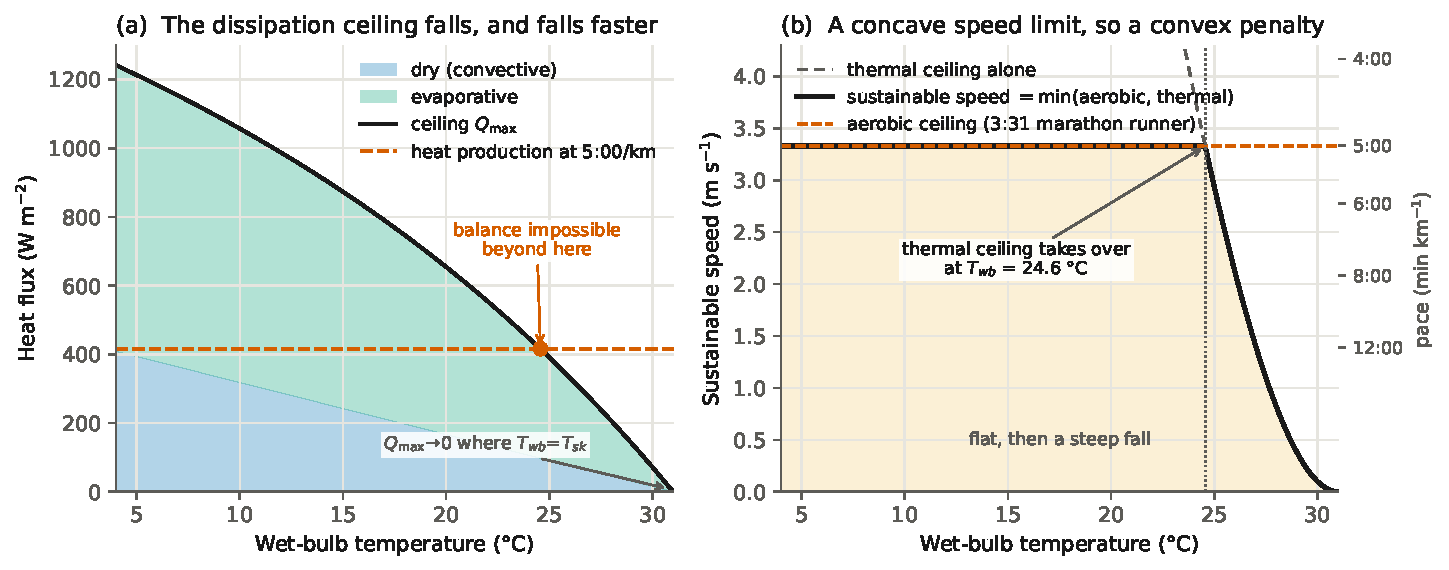
\includegraphics[width=\linewidth]{figures/fig_heat_ceiling.pdf}
  \caption{The heat balance read as a constraint on pace, for the reference
  runner. (a)~The dissipation ceiling $Q_{\max}$ against wet-bulb temperature,
  split into its dry and evaporative parts; the dashed line is the heat the
  runner produces at $5{:}00\,\mathrm{min\,km^{-1}}$. Where the two cross,
  steady-state balance at that pace is no longer available. On this axis the
  dry term never reverses sign, since wetted skin cannot be cooler than the
  wet-bulb temperature. (b)~The speed the balance permits, $v_{\max} \propto
  \Phi^2$, against the runner's own aerobic ceiling. The sustainable speed is
  the lower of the two, so it is flat while the aerobic limit binds and then
  falls steeply. Note that the thermal ceiling takes over only at
  $T_{wb} = 24.6\,^{\circ}$C, roughly WBGT $25$ to $29\,^{\circ}$C depending on
  humidity and solar load, which is far too warm to produce the breakpoint near
  $16\,^{\circ}$C that the learned curve shows; Section~\ref{app:physics:graded}
  takes up what does.}
  \label{fig:heat_ceiling}
\end{figure}

Table~\ref{tab:wbtradeoff} and Figure~\ref{fig:wetbulb_isopleth} walk one
wet-bulb isopleth. Every row sits at $T_{wb} = 22\,^{\circ}$C and is therefore
the same thermal environment by \eqref{eq:qmax-wb}, though assembled quite
differently: the first is a cool morning at $92\%$ humidity, the last desert
heat at $18\%$. As air temperature rises the dry route degrades from shedding
$121$ to \emph{gaining} $152\,\mathrm{W\,m^{-2}}$, reversing sign at
$31\,^{\circ}$C where air and skin are equal, while the drier air widens the
skin-to-air vapour-pressure gradient and evaporative capacity rises by exactly
as much. The trade is exact rather than approximate: along a line of constant
wet-bulb temperature $h_e\,\mathrm{d}P_a = -h_c\,\mathrm{d}T_a$ by definition,
so the two terms move by equal and opposite amounts and their sum cannot shift.
The heavy weight on the wet-bulb term in the definition of WBGT is therefore
recoverable from the heat balance rather than merely calibrated against
outcomes.

\begin{table}[!ht]
\centering\small
\caption{One wet-bulb isopleth, at $T_{wb} = 22\,^{\circ}$C for the reference
runner, with no solar load. Dry and evaporative capacity trade off exactly and
their sum $Q_{\max}$ does not move. The two right-hand columns show what that
invariance does \emph{not} cover: the strain the runner carries, and the fluid
it costs, both rise along the same line. Figure~\ref{fig:wetbulb_isopleth}
draws the same five conditions.}
\label{tab:wbtradeoff}
\begin{tabular}{@{}rrrrrrr@{}}
\toprule
 & & \multicolumn{3}{c}{Heat-loss capacity (W\,m$^{-2}$)}
   & \multicolumn{2}{c}{Cost to the runner} \\
\cmidrule(lr){3-5}\cmidrule(lr){6-7}
Air temp. & Rel.\ hum. & Dry & Evaporative & Total
   & Required & Sweat \\
(\textdegree C) & (\%) & $C$ & $E_{\max}$ & $Q_{\max}$
   & $w_{req}$ & (L\,h$^{-1}$) \\
\midrule
23 & 92 & $+121$ & 434 & 555 & 0.68 & 0.81 \\
29 & 54 & $+30$  & 525 & 555 & 0.74 & 1.06 \\
31 & 45 & $0$    & 555 & 555 & 0.75 & 1.14 \\
35 & 32 & $-61$  & 616 & 555 & 0.78 & 1.31 \\
41 & 18 & $-152$ & 707 & 555 & 0.80 & 1.56 \\
\bottomrule
\end{tabular}
\end{table}

\begin{figure}[!ht]
  \centering
  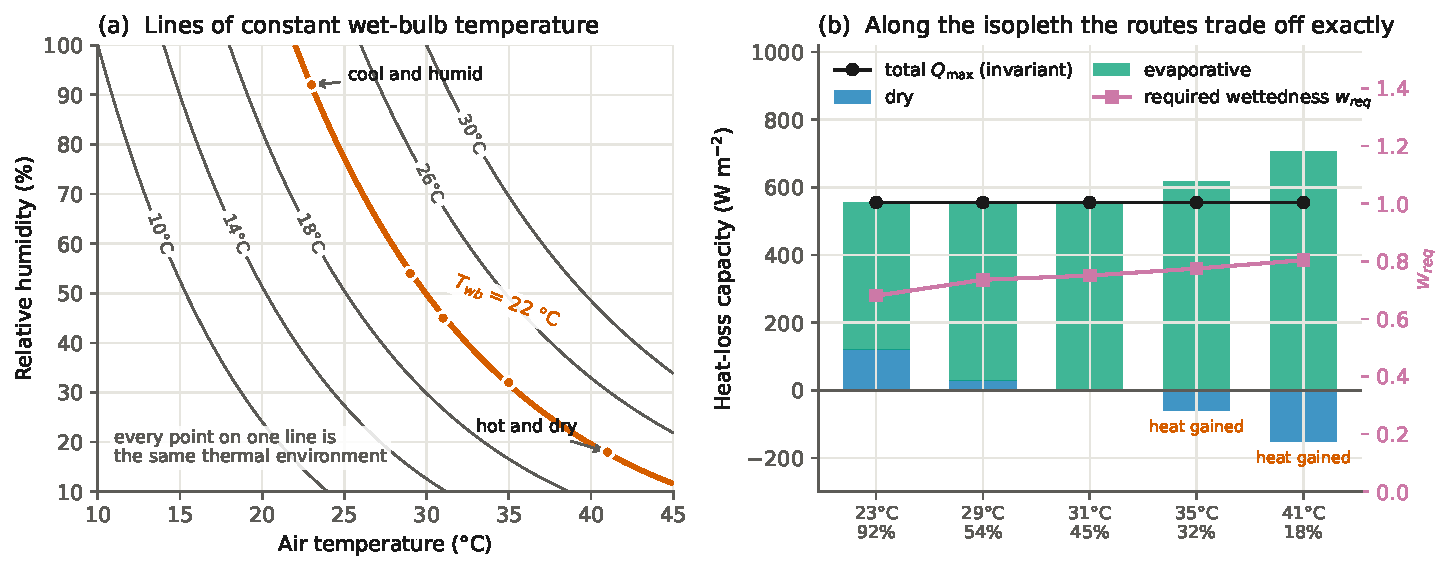
\includegraphics[width=\linewidth]{figures/fig_wetbulb_isopleth.pdf}
  \caption{What a wet-bulb temperature summarizes. (a)~Lines of constant
  $T_{wb}$ on the air-temperature and humidity plane. Any two points on one
  line present the runner with the same dissipation ceiling, which is why a
  single number can stand in for two. The highlighted line carries the five
  conditions of Table~\ref{tab:wbtradeoff}, from a cool humid morning to desert
  heat. (b)~Walking that line: the dry and evaporative routes trade off exactly,
  so their total does not move, but the required wettedness rises anyway. The
  invariance covers the ceiling, not the strain, which is one principled reason
  to expect a model conditioned on WBGT alone to leave residual variance.}
  \label{fig:wetbulb_isopleth}
\end{figure}

The invariance is narrower than it first appears, and the last two columns of
Table~\ref{tab:wbtradeoff} say how. Wet-bulb temperature is a sufficient
statistic for the dissipation \emph{ceiling}, exactly, but not for the
\emph{strain}. Because the runner is a heat source of fixed output, $E_{req} =
H_{prod} - C$ moves with the dry term, so $w_{req} = (H_{prod} - C)/(Q_{\max} -
C)$ is invariant only in the degenerate case $H_{prod} = Q_{\max}$. Along this
isopleth it climbs from $0.68$ to $0.80$, approaching ISO's unacclimatised
limit of $0.85$, while the sweat rate needed to hold pace nearly doubles from
$0.81$ to $1.56\,\mathrm{L\,h^{-1}}$. At matched wet-bulb, hot and dry is
therefore harder on a runner than cool and humid, because the dry route turning
from ally to adversary costs more than the widened vapour-pressure gradient
returns.

\subsection{A concave speed limit makes a convex penalty}
\label{app:physics:convex}

Combining \eqref{eq:pinned} and \eqref{eq:qmax-wb} gives the speed limit
explicitly. Because the transfer coefficients scale with the square root of
running speed, the balance $\kappa v = A\,h_c(v)\,\Phi$ solves in closed form,
\begin{equation}
  v_{\max}(T_{wb}) \;=\; \left(\frac{8.3\,A}{\kappa}\right)^{\!2}\Phi(T_{wb})^{2}
  \;=\; 0.0044\;\Phi(T_{wb})^{2}\ \mathrm{m\,s^{-1}} .
  \label{eq:vmax}
\end{equation}
The pace penalty relative to a cool reference is then
$v_{ref}/v_{\max} - 1$, which is proportional to $\Phi^{-2}$. Differentiating
twice, for any power $p > 0$,
\begin{equation}
  \frac{\mathrm{d}^2}{\mathrm{d}T_{wb}^2}\,\Phi^{-p}
  \;=\; p\,\Phi^{-p-2}\Bigl[(p+1)\,\Phi'^{\,2} \;-\; \Phi\,\Phi''\Bigr]
  \;>\; 0,
  \label{eq:convex-ceiling}
\end{equation}
in which both bracketed terms are positive, the first because it is a square
and the second because $\Phi > 0$ and $\Phi'' < 0$ by \eqref{eq:phi-derivs}.
The pace penalty implied by the ceiling is therefore strictly convex in
wet-bulb temperature. The result does not depend on the constants, on how the
transfer coefficients scale with speed (any $p$ will do, and $p=1$ is the
constant-coefficient case), or on the runner. It requires only that saturation
vapour pressure be increasing and convex, which is thermodynamics rather than
physiology.

Two features of \eqref{eq:vmax} are worth reading off directly.
Figure~\ref{fig:heat_ceiling}(b) draws it. First, the sustainable speed is the
lesser of this thermal limit and the runner's aerobic limit, so the predicted
shape is flat and then falling, which is the qualitative signature the learned
curve shows. Second, the fall has an asymptote rather than a slope: $v_{\max}$
reaches zero at $T_{wb} = T_{sk}$, because at that point the head is zero and
no heat leaves at all. For a runner whose skin sits at $31\,^{\circ}$C that
wall is at a wet-bulb temperature of $31\,^{\circ}$C. It is the running
counterpart of the wet-bulb limit discussed for resting humans
\citep{sherwood2010}, and it is lower for the same reason skin is cooler: running-speed airflow over wet skin holds
the surface below air temperature, and the wall follows the surface down. The
runner's own heat production then ends compensable racing some six degrees
below even that wall. This is why a convex response is the physically expected
one: the constraint does not saturate as conditions worsen, it tightens toward
a vertical asymptote.

Against that, one thing the ceiling argument cannot do is explain the flat band
in the measured curve. For the reference runner the thermal limit overtakes the
aerobic limit only at $T_{wb} = 24.6\,^{\circ}$C, which corresponds to WBGT
between about $25$ and $29\,^{\circ}$C depending on humidity and solar load, and
reading it through required wettedness instead puts the crossing at WBGT $25.7$
to $27.1\,^{\circ}$C depending on whether $w_{\max}$ is taken as ISO's
unacclimatised $0.85$ or an acclimatised $1.0$. Either route is some ten
degrees too warm to account for a breakpoint near $16\,^{\circ}$C. A runner who
held pace until the hard limit bound would show almost no penalty and then a
collapse, which resembles no measured curve. The hard ceiling supplies the
shape of the response but not its onset.

\subsection{Below the ceiling, the same curvature acts on a graded strain}
\label{app:physics:graded}

Runners evidently concede pace long before balance becomes impossible, so the
operative quantity is a graded measure of strain rather than a threshold.
Thermal compensability supplies one. It is $w_{req} = E_{req}/E_{\max}$, where
$E_{req} = H_{prod} - (C + R)$ is the evaporation needed for balance and
$E_{\max}$ the maximum the environment will accept \citep{taylor2006,
belding1955}. Because evaporation scales with wetted area, $w_{req}$ is also
the fraction of the skin that must be covered in sweat, which is what makes it
a graded measure of strain rather than a bare ratio.

Its convexity is the same fact in different clothing, and it is worth being
explicit that this is a corollary rather than an independent finding. The
numerator rises exactly linearly in air temperature, since dry exchange is
proportional to the skin-to-air gradient and simply reverses sign once air
passes skin temperature. The denominator falls at an accelerating rate, for the
one reason given in \eqref{eq:phi-derivs}. Writing $w_{req} = N/D$ with $N$
affine and increasing and $D$ positive, decreasing and concave,
\begin{equation}
  w_{req}'' \;=\; \frac{-\,N D'' D \;-\; 2 N' D' D \;+\; 2 N D'^{2}}{D^{3}},
  \label{eq:convex}
\end{equation}
in which all three numerator terms are positive, since $D'' < 0$, $N' > 0$ and
$D' < 0$. Convexity is therefore a property of the heat balance and not an
artifact of the constants chosen. It is stated here on the air-temperature axis;
because wet-bulb globe temperature is very nearly affine in wet-bulb temperature
over the range plotted---its slope moves only from $1.047$ to $1.042$ across
$10$ to $38\,^{\circ}$C of air temperature---the property carries over to the
axis of Figure~\ref{fig:heat_cost}, which we confirm numerically at relative
humidities from 30 to 90\%.

A proportional response to $w_{req}$ still does not quite describe the measured
curve. Rescaled to match the learned penalty at its endpoints, $w_{req}$
predicts a $0.9\%$ slowdown at $16\,^{\circ}$C WBGT where the learned curve
shows $0.3\%$: strain rises perceptibly in the cool range while measured pace
does not. What reconciles them is a single convex map from strain to conceded
pace. Fitting $\text{penalty} = c\,w_{req}^{\,k}$ over the $16$ to
$28\,^{\circ}$C range returns $k \approx 1.9$, and that one exponent does both
jobs at once: it suppresses the response at low strain, producing the flat band
without a threshold, and it steepens the response at high strain.

The exponent is fitted rather than derived, but it is not unconstrained, and the
bound is the more useful statement. Consider the two natural candidates for what
a runner concedes pace in proportion to. If it is thermal strain itself, the
penalty tracks $w_{req}$, and the predicted steepening over the two bands used
below is $1.80$. If instead it is the fluid cost of sustaining that strain, the
governing quantity is the sweat that must be \emph{produced} rather than the
sweat that evaporates, $w_{req}/\eta_{sw}$, since sweat beyond the evaporative
ceiling drips rather than cools \citep{taylor2006}. Sweating efficiency
$\eta_{sw}$ is itself a measured function of wettedness, falling at fully wetted
skin to $0.50$ under ISO 7933, whose curve follows the working measurements of
\citet{alber1985}, and to $0.67$ under the resting measurements of
\citet{candas1979}; both forms give a predicted steepening near $5$. The
observed $2.18$ lies between the two and nearer the strain end, so runners
appear to concede pace largely in proportion to thermal strain, with a secondary
sensitivity to fluid cost as the skin approaches saturation. Both bounds come
from measured physiology rather than from a free parameter, but a bracket is not
a derivation, and one caveat attaches at the hot end: $w_{req}$ exceeds unity at
$28\,^{\circ}$C for this runner, so both efficiency relations are there being
read beyond the range over which they were established.

\subsection{The same balance, read as a demand on the circulation}
\label{app:physics:circulation}

Nothing above says how heat reaches the skin, and the answer supplies both a
second constraint and a check on the first. Heat is generated in working muscle
and lost at the surface, and the only transport of consequence between them is
convection by blood. That imposes a second balance alongside
\eqref{eq:pinned}: the skin blood flow $\dot{Q}_{sk}$ must carry the whole
production across the core-to-skin temperature gradient,
\begin{equation}
  H \;=\; \rho c_b\,\dot{Q}_{sk}\,\bigl(T_{core} - T_{sk}\bigr)
  \qquad\Longrightarrow\qquad
  \dot{Q}_{sk} \;=\; \frac{H}{\rho c_b\,(T_{core} - T_{sk})},
  \label{eq:skbf}
\end{equation}
with $\rho c_b \approx 3.8\,\mathrm{kJ\,L^{-1}\,K^{-1}}$ the volumetric heat
capacity of blood.\footnote{Published values used in this calculation span
$3.64$ to $4.19\,\mathrm{kJ\,L^{-1}\,K^{-1}}$, the upper end being models that
treat blood as water. The spread does not affect the shape of the result, only
its level.} For the reference runner holding a core temperature of
$39\,^{\circ}$C, this requires at least $1.5\,\mathrm{L\,min^{-1}}$ to the skin
when skin sits at $31\,^{\circ}$C, and at least $3.1$ when it sits at
$35\,^{\circ}$C. \citet{cheuvront2010} run the same calculation for a
world-class marathoner and tabulate the same accelerating pattern, $1.1$,
$2.2$ and $4.4\,\mathrm{L\,min^{-1}}$ as the core-to-skin gradient closes from
$8$ to $4$ to $2\,^{\circ}$C.

These are lower bounds. They credit the skin with the whole production, which
overstates it by the small respiratory share, but they also assume blood
returns from the skin fully cooled to skin temperature, which countercurrent
exchange prevents and which understates the requirement by a good deal more.
The margin is real but not large: cutaneous flow reaches roughly $6$ to
$8\,\mathrm{L\,min^{-1}}$ at rest and plateaus near half of that maximum during
exercise, against a cardiac output that in trained men at exhaustion in the
heat runs near $20\,\mathrm{L\,min^{-1}}$.

Two things follow. The first is the competition the main text refers to. Cardiac
output is finite, and blood directed to the cutaneous beds for cooling is not
available to working muscle, nor does it all return promptly, so a rising
cutaneous demand shows up as some combination of reduced muscle perfusion,
reduced stroke volume with a compensating heart rate, and a compressed
$\dot{V}\mathrm{O}_2$max reserve at unchanged pace. This is the axis
\citet{cheuvront2010} identify, and it is why the strain arrives as
cardiovascular before it arrives as thermal.

The second is structural, and it matters for how the competing accounts in
Section~\ref{app:physics:limits} should be read. The right-hand side of
\eqref{eq:skbf} is a reciprocal of the core-to-skin gradient, so it is convex in
skin temperature for the same elementary reason that $\Phi^{-p}$ is convex in
\eqref{eq:convex-ceiling}: the demand does not rise steadily as the gradient
closes, it accelerates, and it diverges as skin temperature approaches core
temperature. The cardiovascular route therefore carries the same curvature as
the evaporative one, and it must, because the two are consecutive links in one
chain rather than rival mechanisms. Heat that cannot leave the skin raises skin
temperature, which narrows the gradient, which raises the flow required to
deliver the next joule. A convex response is what a chain of this shape
produces regardless of which link is measured, which is a reason to hold the
convexity finding more confidently than any particular mechanism attributed to
it.

\subsection{Why duration matters}
\label{app:physics:duration}

Everything so far has assumed balance. It need not hold instantaneously, since
heat can be stored as a rise in core temperature, and a runner may therefore
hold a pace the environment will not support --- for a while. What that buys is
finite, and pricing it exactly is what separates a marathon from a mile. Taking
tissue heat capacity as $3474\,\mathrm{J\,kg^{-1}\,K^{-1}}$
\citep{burton1935},\footnote{Burton adopted $0.83\,\mathrm{kcal\,kg^{-1}}$ per
degree ``by general custom'' and bounded it only to $0.7$--$0.9$, so the figure
carries perhaps ten percent of slack. The widely quoted $3500$ has no primary
source, and a recent direct measurement of tissue puts it some seventeen
percent lower still. None of this matters here: the storage term is small at
the distance we model, and the argument is that it is small.} the
$2.5\,^{\circ}$C rise a runner will spend in a $70\,\mathrm{kg}$ body is
\begin{equation}
  B \;=\; m\,c\,\Delta T_{core} \;\approx\; 608\,\mathrm{kJ},
  \label{eq:bank}
\end{equation}
a fixed quantity of heat, spent once and not replaced during the race.

The rate at which it is spent is set by the same strain measure as before. Once
$w_{req}$ passes unity the skin cannot get any wetter, so evaporation saturates
at $E_{\max}$ and every further joule is stored:
\begin{equation}
  S \;=\; E_{req} - E_{\max} \;=\; E_{\max}\,\bigl(w_{req} - 1\bigr).
  \label{eq:storage}
\end{equation}
Core temperature then climbs at $S/mc$ and the allowance is exhausted after
$t^{*} = B/S$. Table~\ref{tab:duration} and Figure~\ref{fig:duration_bank}(a)
evaluate this for the reference runner holding
$5{:}00\,\mathrm{min\,km^{-1}}$, and the striking feature is how sharply the
ladder steepens. At $w_{req} = 1.05$ core temperature rises at
$0.6\,^{\circ}\mathrm{C\,h^{-1}}$ and the runner reaches the finish before the
allowance does, so a five percent overshoot is, for practical purposes, free. At
$1.10$ it is spent at $26\,\mathrm{km}$, which is a race that goes wrong late
and not gradually; at $1.25$ at $11\,\mathrm{km}$; at $1.50$ before
$7\,\mathrm{km}$. Nothing in that ladder is a threshold. It is one hyperbola,
$t^{*} \propto (w_{req}-1)^{-1}$, and the flat measured response at cool
temperatures and the steep one at warm are its two ends.

\begin{table}[!ht]
\centering\small
\caption{What the storage allowance of \eqref{eq:bank} buys, for the reference
runner holding $5{:}00\,\mathrm{min\,km^{-1}}$ in air at $60\%$ relative
humidity under $200\,\mathrm{W\,m^{-2}}$ of solar load. Each row is the
environment that puts the runner at that required wettedness. The last row is
the limit in which the environment carries nothing away at all, and its
distance is $d_{bank}$ of \eqref{eq:dbank} --- the floor no runner gets below,
whatever the weather. Figure~\ref{fig:duration_bank} draws both halves.}
\label{tab:duration}
\begin{tabular}{@{}rrrrr@{}}
\toprule
Required & WBGT & Stored & Core rise & Allowance \\
wettedness & (\textdegree C) & $S$ (W) & (\textdegree C\,h$^{-1}$)
   & spent at \\
\midrule
1.05 & 27.5 & 40  & 0.6  & 50.5\,km \\
1.10 & 27.9 & 78  & 1.1  & 26.1\,km \\
1.25 & 28.9 & 177 & 2.6  & 11.5\,km \\
1.50 & 30.1 & 307 & 4.5  & 6.6\,km \\
\midrule
\multicolumn{2}{@{}l}{no dissipation at all} & 770 & 11.4 & 2.6\,km \\
\bottomrule
\end{tabular}
\end{table}

That last row generalises, and it is the cleanest statement in this section.
Suppose the environment carries nothing away, so the whole of production is
stored. The allowance then lasts $B/H$ seconds, and over that time the runner
covers
\begin{equation}
  d_{bank} \;=\; v\,\frac{B}{\kappa\,v} \;=\; \frac{B}{\kappa}
  \;=\; \frac{c\,\Delta T_{core}}{c_{run}} \;\approx\; 2.6\,\mathrm{km}.
  \label{eq:dbank}
\end{equation}
Speed cancels, because production and distance both scale with it. Body mass
cancels too, because the allowance and the cost of covering ground both scale
with that, leaving running economy carried as heat per kilogram per metre,
$c_{run} = \kappa/m \approx 3.3\,\mathrm{J\,kg^{-1}\,m^{-1}}$. What is left is
a distance fixed by three quantities --- tissue heat capacity, the
core-temperature rise the runner is willing to spend, and economy --- and by
nothing whatever about the weather, since the derivation never consulted it. Out to roughly two and a half kilometres, a runner could shed no
heat whatsoever and still finish inside the tolerable rise. Heat cannot bind a
race shorter than that, in any conditions, at any pace, for anybody.

The same cancellation gives the general version. Over a race of distance $d$
the allowance is worth $B/(\kappa d) = d_{bank}/d$ of the runner's total heat
production, again independently of pace and of body mass, which is the curve of
Figure~\ref{fig:duration_bank}(b). It is worth twenty-six times production over
$100\,\mathrm{m}$, $1.75$ times over $1500\,\mathrm{m}$, $88\%$ over
$3000\,\mathrm{m}$, half over $5000\,\mathrm{m}$, a quarter over
$10\,\mathrm{km}$, an eighth over the half marathon and $6\%$ over the marathon.
Read as a fraction of the problem, heat is a rounding error at sprint distances,
a real but secondary term through the middle distances, and essentially the
whole of the problem at the marathon. This is a prediction about where the
constraint switches on, and it is worth noting that it lands on distance rather
than on time.

\begin{figure}[!ht]
  \centering
  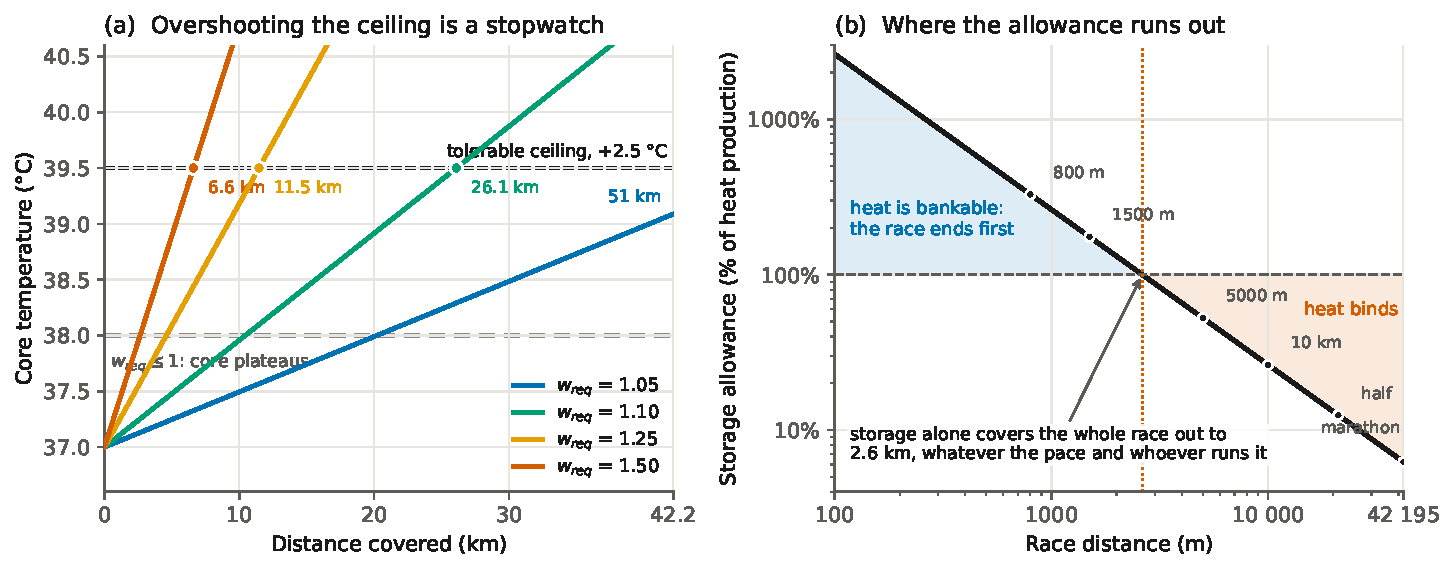
\includegraphics[width=\linewidth]{figures/fig_duration_bank.pdf}
  \caption{Why the same physics governs a marathon and spares a mile.
  (a)~Core temperature against distance covered, for the reference runner
  holding $5{:}00\,\mathrm{min\,km^{-1}}$ at four required wettednesses
  (Table~\ref{tab:duration}); the dot marks where the $2.5\,^{\circ}$C
  allowance is spent and the runner must slow. Below $w_{req} = 1$ balance
  closes and core temperature plateaus instead, so the trajectory never
  arrives. Lines are straight because mean skin temperature is held fixed,
  which makes them optimistic: as the surface balance fails, skin warms, the
  core-to-skin gradient closes and the real trajectory bends upward
  (Section~\ref{app:physics:circulation}). (b)~The allowance as a share of the
  runner's total heat production against race distance. The share is exactly
  $d_{bank}/d$, so the curve is the same for every runner and every pace, and
  it crosses unity at $2.6\,\mathrm{km}$: shorter than that, storage alone
  could absorb the entire race.}
  \label{fig:duration_bank}
\end{figure}

The empirical pattern agrees. \citet{guy2014} report faster sprint performances
in the heat alongside slower marathons. The two halves of that finding are not
in tension: at $100\,\mathrm{m}$ the allowance is twenty-six times production,
so \eqref{eq:dbank} says heat imposes no constraint at all there, which leaves
the ergogenic effect of warmer muscle --- outside this balance, and not
predicted by it --- free to dominate. What the balance does predict is the
distance at which that freedom ends. \citet{leslie2024} find
critical velocity falling $3.7\%$ and then a further $2.9\%$ across heat indices
of $20$, $38$ and $55\,^{\circ}$C --- a \emph{decelerating} response, and the
only regime in this appendix where we predict one, since critical velocity is a
three-to-thirty-minute construct and therefore sits astride $d_{bank}$ where
the storage term still covers most of the imbalance. The same reasoning gives a
reason beyond exposure time why identical conditions cost a slower finisher
more: the allowance is a fixed quantity of heat, so spreading it over a longer
race dilutes it in exactly the proportion $d_{bank}/d$. \citet{taylor2006} list
duration of competition among the determinants of compensability for the same
reason.

Two caveats attach to the trajectories rather than to the accounting. The first
is that the $2.5\,^{\circ}$C allowance is a modelling convention rather than a
measured constant. The rise a runner will accept differs between individuals
and shifts with acclimatisation \citep{periard2015}, and \eqref{eq:dbank} is
exactly proportional to it, so $d_{bank}$ inherits that softness without
attenuation: it is a scale, not a threshold. The second is that holding mean
skin temperature fixed makes
the straight lines of Figure~\ref{fig:duration_bank}(a) the best case. In a
failing balance the skin warms, which narrows the core-to-skin gradient and
raises the blood flow required to move the next joule
(Section~\ref{app:physics:circulation}), so the real trajectory accelerates and
the distances in Table~\ref{tab:duration} are upper bounds. Both caveats push
the same way, which is toward heat binding sooner than tabulated, not later.

\subsection{Does it predict the curvature we measured?}
\label{app:physics:curvature}

Between the $20$--$24$ and $24$--$28\,^{\circ}$C WBGT bands the learned curve of
Section~\ref{sec:results} steepens by a factor of $2.18$. Evaluated over the
same bands, $w_{req}$ alone steepens by $1.80$, and across relative humidities
of $40$--$85\%$ and solar loads of $0$--$500\,\mathrm{W\,m^{-2}}$ the predicted
factor spans $1.5$ to $2.7$. The prediction brackets the observation, and the
direction of any residual gap is the expected one: with a convex strain-to-pace
map the heat balance supplies a lower bound on curvature, not an equality.

The prediction is robust to most of its inputs and fragile in one. Varying the
convective coefficient across the full published span at this speed, $10.4$ to
$33.7\,\mathrm{W\,m^{-2}\,K^{-1}}$, moves the predicted factor only to
$1.4$--$2.8$; varying metabolic rate from a $60\,\mathrm{kg}$ runner at
$5{:}00\,\mathrm{min\,km^{-1}}$ to a $70\,\mathrm{kg}$ runner at $4{:}00$ moves
it to $1.5$--$2.8$. Mean skin temperature dominates instead. At the
laboratory-running value of $35\,^{\circ}$C the prediction falls to $1.3$--$1.8$
and misses the observation; at $29\,^{\circ}$C it widens to $1.6$--$4.3$. We
adopt $31\,^{\circ}$C because \citet{aylwin2023} measured mean skin temperature
falling from $29.8$ to $28.9\,^{\circ}$C through the men's marathon at the 2019
World Championships, below air temperature and well below laboratory treadmill
values, with running-speed airflow over wet skin the reason.

That measurement carries a caveat which cuts against us and is worth stating.
Aylwin's thermography covers exposed skin, some $64\%$ of body surface area,
while the heat balance wants a whole-body mean that includes covered skin, which
runs warmer. Weighting the covered remainder at anything from $32$ to
$38\,^{\circ}$C puts the whole-body mean between $30.3$ and $32.5\,^{\circ}$C,
over which range the predicted factor spans $1.4$ to $3.1$ and continues to
bracket the observation; the prediction fails only above about
$33\,^{\circ}$C, which no plausible weighting of these measurements reaches. The
agreement is therefore correct in sign and order of magnitude but not sharp, and
the width of the band is dominated by a quantity the corpus does not observe.

\subsection{Does the penalty survive on the thermometer's axis?}
\label{app:physics:drybulb}

Everything so far is stated on a humidity-weighted axis, which invites the
objection that the finding is a property of the index rather than of the
weather. It is not, and separating the two yields the sharpest prediction in
this appendix.

Hold relative humidity fixed and vary air temperature. The head becomes
$\Phi(T_a) = (T_{sk} - T_a) + \mathrm{LR}\,(P_s(T_{sk}) - \mathrm{RH}\cdot
P_s(T_a))$, so
\begin{equation}
  \Phi''(T_a) \;=\; -\,\mathrm{LR}\cdot\mathrm{RH}\cdot P_s''(T_a).
  \label{eq:phi-rh}
\end{equation}
The curvature is not merely humidity-sensitive; it is exactly proportional to
relative humidity, and it vanishes identically in perfectly dry air. The
consequence for the graded measure is stark and is drawn in
Figure~\ref{fig:drybulb_axis}(a): $w_{req}$ is a strictly convex function of air
temperature at every humidity we can race in, and an exactly linear one at
$\mathrm{RH} = 0$, where its denominator stops depending on air temperature
altogether. All of the acceleration in the strain measure is a humidity effect
wearing a temperature label.

The two measures part company here, which makes the dry end a discriminating
test rather than a curiosity. The ceiling penalty retains a residual convexity
even in dry air, because a reciprocal of an affine function is still convex, so
it predicts a mild bend where $w_{req}$ predicts none: at $25\,^{\circ}$C and
zero humidity the penalty's second derivative is $1.6\times10^{-4}$ against
$5.3\times10^{-3}$ at $50\%$ and $7.3\times10^{-2}$ at $90\%$. A corpus with
enough genuinely hot and dry racing would separate the two accounts. Ours does
not contain it.

Finally, the practical question. Because the model was shown wet-bulb globe
temperature and nothing else, it cannot be asked directly what an extra degree
of dry-bulb heat costs; but the learned curve can be composed with the map from
$(T_a, \mathrm{RH})$ to WBGT and read on the thermometer's axis, which is
Figure~\ref{fig:drybulb_axis}(b) and Table~\ref{tab:drybulb}. The slowdown does
not depend on the index for its existence. At $50\%$ humidity and a solar load
of $200\,\mathrm{W\,m^{-2}}$, warming from $10$ to $25\,^{\circ}$C of air
temperature costs $1.7\%$ of pace, and warming to $30\,^{\circ}$C costs $3.7\%$;
the same $25\,^{\circ}$C day costs $1.0\%$ at $30\%$ humidity and $3.5\%$ at
$90\%$. The penalty rises monotonically along every constant-humidity line, and
it accelerates along each of them, so the shape reported in
Section~\ref{sec:results} is a property of the weather rather than of the
weighting. What the composition also shows is how much the thermometer alone
conceals: a single air temperature spans a threefold range of cost depending on
the humidity attached to it, which is the practical case for carrying the
composite index rather than the raw reading.

\begin{figure}[!ht]
  \centering
  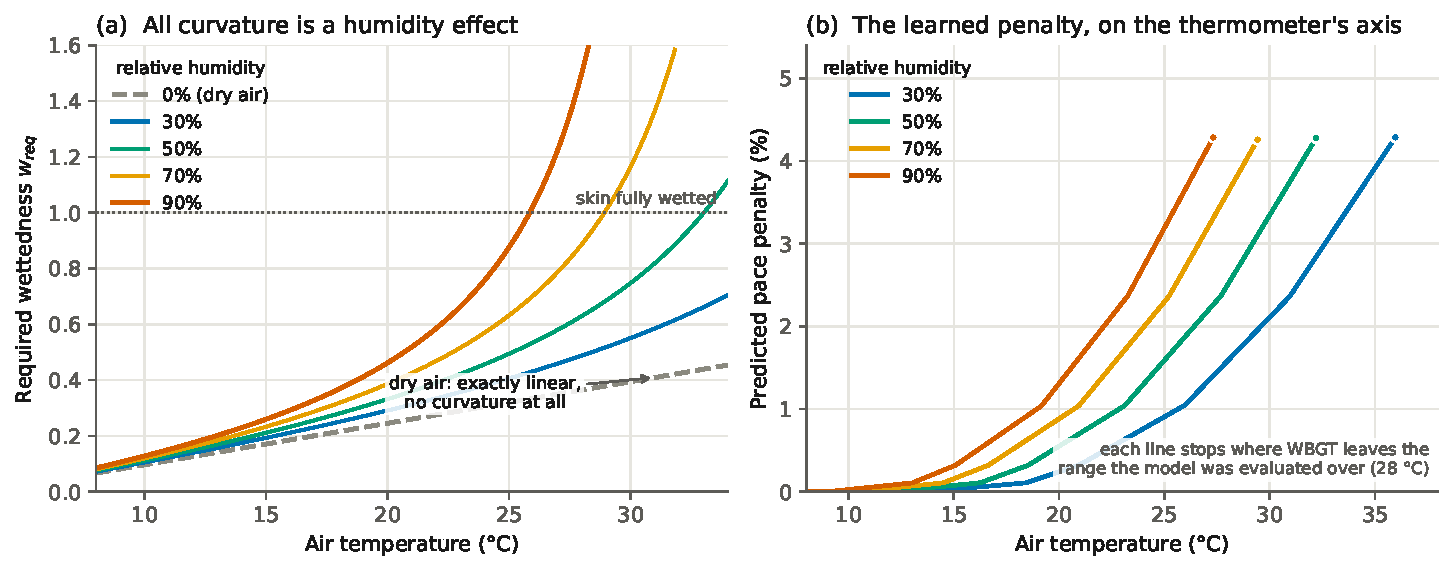
\includegraphics[width=\linewidth]{figures/fig_drybulb_axis.pdf}
  \caption{The response on the dry-bulb axis, at fixed relative humidity.
  (a)~Required wettedness against air temperature. The curvature is exactly
  proportional to humidity by \eqref{eq:phi-rh}, so the dry-air case is a
  straight line and every other case bends; the acceleration in the strain
  measure is entirely a humidity effect. (b)~The learned population curve of
  Figure~\ref{fig:heat_cost} composed with the map from air temperature and
  humidity to WBGT, at a solar load of $200\,\mathrm{W\,m^{-2}}$ and
  $1\,\mathrm{m\,s^{-1}}$ of wind. Each line stops where WBGT leaves the range
  over which the model was evaluated. Drawn by linear interpolation of the
  anchor values reported in Section~\ref{sec:results}, which is the source of
  the visible kinks.}
  \label{fig:drybulb_axis}
\end{figure}

\begin{table}[!ht]
\centering\small
\caption{The learned penalty re-expressed on the dry-bulb axis: percent pace
slowdown relative to $10\,^{\circ}$C of air temperature at the same humidity,
with a solar load of $200\,\mathrm{W\,m^{-2}}$ and $1\,\mathrm{m\,s^{-1}}$ of
wind. Dashes mark conditions whose WBGT exceeds $28\,^{\circ}$C, beyond the
range the model was evaluated over. Reading across a row isolates the cost of
humidity at fixed temperature; reading down a column isolates the cost of
temperature at fixed humidity.}
\label{tab:drybulb}
\begin{tabular}{@{}rrrrr@{}}
\toprule
Air temp. & \multicolumn{4}{c}{Relative humidity} \\
\cmidrule(lr){2-5}
(\textdegree C) & 30\% & 50\% & 70\% & 90\% \\
\midrule
10 & 0.00 & 0.00 & 0.00 & 0.03 \\
15 & 0.03 & 0.10 & 0.18 & 0.29 \\
20 & 0.24 & 0.59 & 1.00 & 1.45 \\
25 & 1.03 & 1.70 & 2.34 & 3.53 \\
30 & 2.17 & 3.74 & --- & --- \\
\bottomrule
\end{tabular}
\end{table}

\subsection{What this does and does not establish}
\label{app:physics:limits}

The argument constrains shape, not magnitude: nothing here derives the $5.0\%$
penalty of Section~\ref{sec:results}. What it does establish is narrower and
more durable. Convexity in the response is a theorem about the heat balance
rather than a feature fitted to the data, it holds on the ceiling and on the
graded strain measure alike, it survives the change of axis from wet-bulb to
WBGT and to dry-bulb at fixed humidity, and it traces in every case to one
term, $P_s''$. A linear penalty is not a simplification of this physics; it is
inconsistent with it.

Two competing explanations for the same curvature deserve naming, since neither
is excluded by our data. \citet{cheuvront2010} attribute an exponential decline
in aerobic performance to the cardiovascular axis; as
Section~\ref{app:physics:circulation} argues, that account shares the structure rather than
competing with it, but the two make different predictions about which
intervention helps and cannot be separated here. \citet{wang2024} attribute more
than half the marathon heat effect to reduced atmospheric oxygen partial
density, since warm air expands and rising vapour pressure displaces oxygen, a
mechanism that also scales with vapour pressure and therefore mimics the
humidity signature of the evaporative account while fitting a
piecewise-\emph{linear} form. Distinguishing the three requires measurements
this corpus does not contain.

A statistical objection applies to any pooled curve. Because the penalty is
strongly ability-dependent \citep{ely2007}, differential slopes combined with
differential field composition across warm and cool races can bend an aggregate
curve while no individual curve is convex. Our design is partly protected: the
curve of Section~\ref{sec:results} is the median of \emph{per-runner}
counterfactual sweeps, in which each runner's own response is traced with every
other channel held fixed, rather than a regression pooled across runners and
races. It is not protected against the possibility that the deep model has
learned one population-average response and applies it uniformly.

Finally, the critical wet-bulb temperature at running metabolic rates appears
not to have been measured. \citet{wolf2021} report critical WBGT falling from
$35.3\,^{\circ}$C at rest to $31.6\,^{\circ}$C at $30\%$
$\dot{V}\mathrm{O}_2$max, about $163\,\mathrm{W\,m^{-2}}$, while a marathon runs
above $400\,\mathrm{W\,m^{-2}}$. Occupational limit curves extrapolated that far
give $22\,^{\circ}$C WBGT (ACGIH) or $18\,^{\circ}$C (NIOSH), far below
conditions marathons are routinely held in, which suggests those curves do not
transfer to self-paced athletic work. Equation~\eqref{eq:vmax} makes the same
point from the other direction: it places an absolute wall at $T_{wb} = T_{sk}$
and, for the reference runner, an end to compensable racing some six degrees
below it. Neither number has been measured in runners. The gap is worth naming
as a target for measurement rather than filled by extrapolation here.

The calculations in this appendix are reproduced by
\texttt{verify\_heat\_convexity.py}, which is self-checking and prints a pass or
fail line for every number quoted above; the figures are built by
\texttt{build\_compensability\_figures.py}.


\end{document}
